% Created 2025-07-25 Fr 14:56
% Intended LaTeX compiler: pdflatex
\documentclass{mimosis}
\usepackage[utf8]{inputenc}
\usepackage[T1]{fontenc}
\usepackage{graphicx}
\usepackage{longtable}
\usepackage{wrapfig}
\usepackage{rotating}
\usepackage[normalem]{ulem}
\usepackage{amsmath}
\usepackage{amssymb}
\usepackage{capt-of}
\usepackage{hyperref}
%%%%%%%%%%%%%%%%%%%%%%%%%%%%%%%%%%%%%%%%%%%%%%%%%%%%%%%%%%%%%%%%%%%%%%%%%%%%%%%%
% Colors
%%%%%%%%%%%%%%%%%%%%%%%%%%%%%%%%%%%%%%%%%%%%%%%%%%%%%%%%%%%%%%%%%%%%%%%%%%%%%%%%

% University
\definecolor{UoTred}{RGB}{165,30,55}
\definecolor{UoTdark}{RGB}{50,65,75}
\definecolor{UoTgold}{RGB}{180,160,105}
\definecolor{UoTgray}{RGB}{185,184,188}
\definecolor{UoTdarkblue}{RGB}{65,90,140}
\definecolor{UoTblue}{RGB}{0,105,170}
\definecolor{UoTlightblue}{RGB}{80,170,200}
\definecolor{UoTlightgreen}{RGB}{125,165,75}
\definecolor{UoTgreen}{RGB}{125,165,75}
\definecolor{UoTdarkgreen}{RGB}{50,110,30}
\definecolor{UoTlightred}{RGB}{200,80,60}
\definecolor{UoTpurple}{RGB}{175,110,150}
\definecolor{UoTorange}{RGB}{210,150,0}

% TUM
\definecolor{TUMblue}{RGB}{0,101,189}
\definecolor{TUMDarkBlue}{RGB}{0,82,147}
\definecolor{TUMLightBlue}{RGB}{100,160,200}
\definecolor{TUMLighterBlue}{RGB}{152,198,234}
\definecolor{TUMorange}{RGB}{227,114,34}
\definecolor{TUMgreen}{RGB}{162,173,0}

% Aalto
\definecolor{aaltoyellow}{cmyk}{0,0,75,0}

% Julia
\definecolor{jblue}{rgb}{0.251,0.388,0.847}
\definecolor{jgreen}{rgb}{0.22,0.596,0.149}
\definecolor{jpurple}{rgb}{0.584,0.345,0.698}
\definecolor{jred}{rgb}{0.796,0.235,0.2}

\colorlet{maincolor}{UoTblue}

\colorlet{allboxcolor}{UoTblue}
\colorlet{algboxcolor}{UoTpurple}
\colorlet{propositionboxcolor}{allboxcolor}
\colorlet{corollaryboxcolor}{allboxcolor}
\colorlet{definitionboxcolor}{allboxcolor}
\colorlet{exampleboxcolor}{UoTgreen}
\colorlet{remarkboxcolor}{UoTdarkblue}

%%%%%%%%%%%%%%%%%%%%%%%%%%%%%%%%%%%%%%%%%%%%%%%%%%%%%%%%%%%%%%%%%%%%%%%%%%%%%%%%
% Font settings
%%%%%%%%%%%%%%%%%%%%%%%%%%%%%%%%%%%%%%%%%%%%%%%%%%%%%%%%%%%%%%%%%%%%%%%%%%%%%%%%

% \setmainfont{LibreBaskerville}
% \setsansfont{IBM Plex Sans}
% \setmonofont{IBM Plex Mono}

% \usepackage{baskervaldx}

\usepackage[defaultsans]{lato}
% \usepackage{lmodern}
\usepackage{anyfontsize}

% Set KOMA fonts for book-specific elements
\addtokomafont{part}{\normalfont\scshape\bfseries\sffamily}
\addtokomafont{partentry}{\normalfont\scshape\bfseries}
\addtokomafont{chapter}{\normalfont\bfseries}
\addtokomafont{chapterentry}{\normalfont\bfseries}

% Set KOMA fonts for elements common to all classes
\addtokomafont{section}{\normalfont\bfseries}
\addtokomafont{subsection}{\normalfont\bfseries}
\addtokomafont{subsubsection}{\normalfont\bfseries}
\addtokomafont{paragraph}{\normalfont\bfseries}
\setkomafont{descriptionlabel}{\normalfont\bfseries}

\addtokomafont{chapter}{\normalfont\sffamily}
\addtokomafont{chapterprefix}{\normalfont\sffamily}
\addtokomafont{section}{\normalfont\sffamily}
\addtokomafont{subsection}{\normalfont\sffamily}
\addtokomafont{subsubsection}{\normalfont\sffamily}


%%%%%%%%%%%%%%%%%%%%%%%%%%%%%%%%%%%%%%%%%%%%%%%%%%%%%%%%%%%%%%%%%%%%%%%%%%%%%%%%
% Packages
%%%%%%%%%%%%%%%%%%%%%%%%%%%%%%%%%%%%%%%%%%%%%%%%%%%%%%%%%%%%%%%%%%%%%%%%%%%%%%%%
\usepackage{minted}
\usepackage[capitalize,noabbrev]{cleveref}
\crefname{equation}{eq.}{eqs.}
\usepackage{physics}
\usepackage{lipsum}
\usepackage{nccmath}
\usepackage{mathtools}
\usepackage{bbm}
\usepackage{enumitem}
\usepackage{etoc}
\usepackage{svg}

\usepackage{pdfpages}
\newcommand{\fakesection}[1]{%
  \par\refstepcounter{section}% Increase section counter
  \sectionmark{#1}% Add section mark (header)
  \addcontentsline{toc}{section}{\protect\numberline{\thesection}#1}% Add section to ToC
  % Add more content here, if needed.
}
\newcommand{\includepaper}[3]{
  \cleardoublepage
  \includepdf[
    pages=1,
    pagecommand={\fakesection{#2}\label{#3}},
    fitpaper,
    % frame=true,
    noautoscale,
    height=1.13\textheight,
  ]{#1}
  \includepdf[
    pages=2-,
    pagecommand={},
    fitpaper,
    % frame=true,
    noautoscale,
    height=1.13\textheight,
  ]{#1}
}


\usepackage[most]{tcolorbox}
\tcbset{simplebox/.style={
  unbreakable,
  colback=gray!10,
  sharp corners=all,
  boxrule=0.5pt,
}}


\usepackage[noEnd=false]{algpseudocodex}
\usepackage{algorithm}
\newenvironment{myalgorithm}{\algorithm}{\endalgorithm}
\tcolorboxenvironment{myalgorithm}{
  simplebox,
  left=10pt,
  right=10pt,
  top=0pt,
  bottom=10pt,
}


\usepackage[
  background=allboxcolor,
  backgroundopacity=10,
  theorembackground=theoremboxcolor,
  propositionbackground=propositionboxcolor,
  lemmabackground=lemmaboxcolor,
  corollarybackground=corollaryboxcolor,
  definitionbackground=definitionboxcolor,
  assumptionbackground=assumptionboxcolor,
  remarkbackground=remarkboxcolor,
  examplebackground=exampleboxcolor,
  exercisebackground=exerciseboxcolor,
  algbackground=algboxcolor,
]{kaotheorems}


\usepackage{tikz}
\usetikzlibrary{bayesnet}
\usetikzlibrary{positioning}
\usetikzlibrary{calc}

% \usepackage[%
\hypersetup{%
  colorlinks = true,
  citecolor  = UoTdarkblue,
  linkcolor  = UoTdarkblue,
  urlcolor   = UoTdarkblue,
  unicode,
  linktocpage=true,
}
\PassOptionsToPackage{unicode}{hyperref}
\PassOptionsToPackage{naturalnames}{hyperref}

\usepackage[%
  backend=biber,
  % style=apa,
  style=numeric,
  maxbibnames=99,
  maxcitenames=1,
  uniquename=init,
  uniquelist=false,
  url=false,
  % date=year,
  doi=false,
  ]{biblatex}
  \AtEveryBibitem{\clearfield{month}}
  % \AtEveryBibitem{\clearfield{url}}
  \AtEveryBibitem{\clearfield{editor}}
  % \AtEveryBibitem{\clearfield{eprint}}
  % \AtEveryBibitem{\clearfield{pages}}
  % \AtEveryBibitem{\clearfield{volume}}

  % \usepackage[%
  % skip=5.5pt,%
  % ]{parskip}


\newcommand{\capos}{\hyperlink{capos}{Publication I}}
\newcommand{\pickandmix}{\hyperlink{pickandmix}{Publication II}}
\newcommand{\highdim}{\hyperlink{highdim}{Publication III}}
\newcommand{\fenrir}{\hyperlink{fenrir}{Publication IV}}
\newcommand{\probexpint}{\hyperlink{probexpint}{Publication V}}
\newcommand{\tempering}{\hyperlink{tempering}{Publication VI}}
\newcommand{\pint}{\hyperlink{pint}{Publication VII}}
\newcommand{\joss}{\hyperlink{joss}{Publication VIII}}
\newcommand{\publications}[1]{\hyperlink{listofpublications}{Publications #1}}
\newcommand{\scapos}{\hyperlink{capos}{I}}
\newcommand{\spickandmix}{\hyperlink{pickandmix}{II}}
\newcommand{\shighdim}{\hyperlink{highdim}{III}}
\newcommand{\sfenrir}{\hyperlink{fenrir}{IV}}
\newcommand{\sprobexpint}{\hyperlink{probexpint}{V}}
\newcommand{\stempering}{\hyperlink{tempering}{VI}}
\newcommand{\spint}{\hyperlink{pint}{VII}}
\newcommand{\sjoss}{\hyperlink{joss}{VIII}}

  %%%%%%%%%%%%%%%%%%%%%%%%%%%%%%%%%%%%%%%%%%%%%%%%%%%%%%%%%%%%%%%%%%%%%%%%%%%%%%%%
  % Utilities
  %%%%%%%%%%%%%%%%%%%%%%%%%%%%%%%%%%%%%%%%%%%%%%%%%%%%%%%%%%%%%%%%%%%%%%%%%%%%%%%%
\newcommand{\equalc}{\textsuperscript{*}}

\newcommand{\chapterbasedonbox}[1]{%
  \begin{tcolorbox}[
    colback=gray!10,
    % colframe=UoTblue,
    % sharp corners=all,
    % boxrule=0.5pt,
    % before skip=\topskip,
    % after skip=\topskip,
    % left skip=0pt,
    % right skip=0pt,
    left=3pt,
    right=3pt,
    % top=5pt,
    % bottom=3pt,
    boxrule=1pt,
    ]
    #1
  \end{tcolorbox}
}
\newcommand{\chapterbasedon}[2]{%
  \chapterbasedonbox{\textbf{This chapter is based on #1:}
    \begin{itemize}[
      left=0pt .. 1em,
      topsep=3pt,
      itemsep=3pt,
      parsep=0pt,
      ]
      \item[] #2
    \end{itemize}
  }
}


\newcommand{\algeqspacing}{%
\setlength{\belowdisplayskip}{3pt}
\setlength{\belowdisplayshortskip}{2pt}
\setlength{\abovedisplayskip}{3pt}
\setlength{\abovedisplayshortskip}{-8pt}
}

\newcommand{\wrapupsec}{Conclusion}

%%%%%%%%%%%%%%%%%%%%%%%%%%%%%%%%%%%%%%%%%%%%%%%%%%%%%%%%%%%%%%%%%%%%%%%%%%%%%%%%
% Layout things
%%%%%%%%%%%%%%%%%%%%%%%%%%%%%%%%%%%%%%%%%%%%%%%%%%%%%%%%%%%%%%%%%%%%%%%%%%%%%%%%
\renewcommand\contentsname{Table of Contents}
\addto\captionsenglish{% Replace "english" with the language you use
  \renewcommand{\contentsname}%
    {Table of Contents}%
}

% \setcounter{tocdepth}{1}

\makeatletter
\newcommand\matter@switch{}
\addtokomafont{chapterentry}{\matter@switch}
\g@addto@macro\frontmatter{%
  \addtocontents{toc}{%
    \protect\renewcommand\protect\matter@switch{\normalfont\itshape}%
  }%
}
\g@addto@macro\mainmatter{%
  \addtocontents{toc}{%
    \protect\renewcommand\protect\matter@switch{}%
  }%
}
\makeatother

% TOC: Parts in colour
\newcommand\tocpartstyle[1]{%
  \scshape\large\bfseries\textcolor{maincolor}{#1}}
\DeclareTOCStyleEntries[pagenumberwidth=2.5em, entryformat=\tocpartstyle]{tocline}{part}


%%%%%%%%%%%%%%%%%%%%%%%%%%%%%%%%%%%%%%%%
% Tikx in figure captions
%%%%%%%%%%%%%%%%%%%%%%%%%%%%%%%%%%%%%%%%

% Coloured dashed line
\DeclareRobustCommand{\dashedcolorline}[1]{%
	\begin{tikzpicture}
		\raisebox{1.5pt}{
			\draw[#1,dashed,line width=1.5pt] (0,0) -- (1em,0);
		}
	\end{tikzpicture}%
}
\DeclareRobustCommand{\colordot}[1]{%
	\begin{tikzpicture}[baseline=(a.south)]
		\node[circle, scale=0.75,color=white, fill=#1] (a) {};
	\end{tikzpicture}%
}

\newenvironment{proofsketch}{\textit{Sketch of the proof.}}{\hfill$\square$}

% \newcommand{\tr}{\operatorname{tr}}
\newcommand{\T}{\top}
\newcommand{\logdet}[1]{\log \left| #1 \right|}


% \newcommand{\vect}[1]{\mathbf{#1}}
% \newcommand{\mat}[1]{\bm{#1}}
\newcommand{\vect}[1]{#1}
\newcommand{\mat}[1]{#1}

\newcommand{\R}{\mathbb{R}}
\newcommand{\eye}{\mat{I}}
\newcommand{\I}[1]{\mat{I}_{#1}}
\DeclareMathOperator*{\argmax}{arg\,max}
\newcommand{\Z}{\mathcal{Z}}

\DeclareDocumentCommand\dirac{}{\opbraces{\delta}}
\DeclareDocumentCommand\p{}{\opbraces{p}}
\DeclareDocumentCommand\q{}{\opbraces{q}}
\DeclareDocumentCommand\N{}{\opbraces{\mathcal{N}}}
\DeclareDocumentCommand\GP{}{\opbraces{\mathcal{GP}}}
\DeclareDocumentCommand\dirac{}{\opbraces{\delta}}
\DeclareDocumentCommand\E{}{\opbraces{\mathbb{E}}}
\DeclareDocumentCommand\C{}{\opbraces{\mathbb{C}}}

\DeclareDocumentCommand\tria{}{\opbraces{\operatorname{tria}}}
\DeclareDocumentCommand\diag{}{\opbraces{\operatorname{diag}}}


\newcommand{\jac}[1]{J_{#1}}
% \newcommand{\jac}[2]{J_{#1}(#2)}
% \newcommand{\jac}[2]{\eval{\pdv{#1}{x}}_{x=#2}}


%%%%%%%%%%%%%%%%%%%%%%%%%%%%%%%%%%%%%%%%%%%%%%%%%%%%%%%%%%%%%%%%%%%%%
% My notation
%%%%%%%%%%%%%%%%%%%%%%%%%%%%%%%%%%%%%%%%%%%%%%%%%%%%%%%%%%%%%%%%%%%%%
\newcommand{\sval}{y} % the ODE solution (scalar)
\newcommand{\vval}{\vect{y}} % the ODE solution (vector)
\newcommand{\val}{\sval}
\newcommand{\st}{x} % the SSM representation
\newcommand{\vobs}{\vect{z}} % the SSM observations (vector)
\newcommand{\sobs}{z} % the SSM observations (scalar)
\newcommand{\obs}{\sobs}
\newcommand{\oobs}{u}

\newcommand{\mean}[1]{\vect{\mu}_{#1}} %
\newcommand{\cov}[1]{\mat{\Sigma}_{#1}} %
\newcommand{\covb}[1]{\breve{\mat{\Sigma}}_{#1}}

\newcommand{\gpmeanfun}{m}
\newcommand{\gpcovfun}{k}
\newcommand{\gpcovmat}{\mat{K}}

% \newcommand{\stmean}{\mean{\st}} %
% \newcommand{\stcov}{\cov{\st}} %
% \newcommand{\obsmean}{\mean{\obs}} %
% \newcommand{\obscov}{\cov{\obs}} %

\newcommand{\drift}{\mat{F}} %
\newcommand{\disp}{\mat{\Gamma}^{1/2}} %
\newcommand{\dispb}{\breve{\mat{\Gamma}}^{1/2}} %
\newcommand{\dispc}{\check{\mat{\Gamma}}^{1/2}} %
\newcommand{\dispsq}{\mat{\Gamma}} %
\newcommand{\wiener}{\vect{w}} %
\newcommand{\proj}[1]{\mat{E}_{#1}} %
% \newcommand{\diff}{\sigma}
\newcommand{\sdiff}{\sigma}
\newcommand{\Diff}{\Xi^{1/2}}
\newcommand{\DiffHat}{\hat{\Xi}^{1/2}}
\newcommand{\DiffSq}{\Xi}
\newcommand{\DiffBase}{\Xi}
\newcommand{\DiffMLE}{\hat{\Xi}^{1/2}_\text{MLE}}

\newcommand{\IWP}[1]{\ensuremath{\operatorname{IWP}(#1)}}
\newcommand{\IOUP}{\ensuremath{\operatorname{IOUP}}}

\newcommand{\transf}{f} %
\newcommand{\transA}{\mat{A}} %
\newcommand{\transb}{\vect{b}} %
\newcommand{\transC}{\mat{Q}} %
\newcommand{\obsh}{h} %
\newcommand{\obsA}{\mat{H}} %
\newcommand{\obsb}{\vect{c}} %
\newcommand{\obsC}{\mat{R}} %
\newcommand{\outA}{\mat{E}} %

\newcommand{\invtransA}{\mat{G}} %
\newcommand{\invtransb}{\vect{d}} %
\newcommand{\invtransC}{\mat{\Lambda}} %

\newcommand{\numparams}{K}
\newcommand{\numdims}{d}
\newcommand{\numderviatives}{q}
\newcommand{\numstates}{D}
\newcommand{\numtimes}{N}
\newcommand{\numdata}{M}
\newcommand{\numtemperingsteps}{n}

\newcommand{\dt}{{\Delta t}}
\newcommand{\tindex}{n}
\newcommand{\idxt}{\tindex}
\newcommand{\tindexmax}{N}
\newcommand{\idxtmax}{\tindexmax}

\newcommand{\data}{\mathcal{D}}

\DeclareDocumentCommand\PNML{}{\widehat{\mathcal{M}}_\text{PN}}
\DeclareDocumentCommand\ML{}{\mathcal{M}}
\newcommand{\MLE}[1]{\hat{#1}_\text{MLE}}

\DeclareDocumentCommand\vf{}{\opbraces{f}}

\addbibresource{references.bib}
\author{Nathanael Bosch}
\date{\today}
\title{A Flexible and Efficient Framework for Probabilistic Numerical Simulation and Inference}
\begin{document}

\frontmatter
\begin{titlepage}
  \vspace*{2cm}
  \makeatletter
  \begin{center}
  %
  \sffamily
    \begin{huge}
      % \@title
      % Developing Flexible and Efficient Probabilistic Numerical Solvers for Ordinary Differential Equations
      A Flexible and Efficient Framework for\\[0.5em] Probabilistic Numerical Simulation and Inference
      % Developing a Flexible and Efficient Framework for Probabilistic Numerical Simulation and Inference
      %Towards a Flexible and Efficient Framework for\\[0.5em] Probabilistic Numerical Simulation and Inference
      % Bayesian Filtering as a Flexible and Efficient Framework for Probabilistic Numerical ODE Solvers
    \end{huge}\\[0.1cm]
    %
    \vfill
    %
    {\bfseries Dissertation}\\[0pt]
			%\vspace*{5pt}
			{%\sffamily
				der Mathematisch-Naturwissenschaftlichen Fakultät\\
				der Eberhard Karls Universität Tübingen\\
				zur Erlangung des Grades eines\\
				Doktors der Naturwissenschaften\\
				(Dr.\ rer.\ nat.)}
    %
    \vfill
    %
    vorgelegt von\\
    \@author\\
    aus Stuttgart
    %
    \vfill
    %
    Tübingen\\
    2024
  \end{center}
  \makeatother
\end{titlepage}

\clearpage\normalsize
%
\thispagestyle{empty}{\raggedright\null\vfill
\sffamily
Gedruckt mit Genehmigung der Mathematisch-Naturwissenschaftlichen Fakultät der
Eberhard Karls Universität Tübingen.\par\bigskip\bigskip\bigskip\noindent
\begin{tabular}{@{}ll}
Tag der m\"{u}ndlichen Qualifikation: \qquad\qquad\qquad & 26.02.2025 \\
Dekan: & Prof. Dr. Thilo Stehle \\
1. Berichterstatter: & Prof. Dr. Philipp Hennig \\
2. Berichterstatter: & Dr. Jon Cockayne \\
%3. Berichterstatter: & \\
\end{tabular}
}
\clearpage


\thispagestyle{empty}
\newpage
\chapter{Abstract}
\label{sec:orgfc790a0}

\emph{Probabilistic numerics} has emerged as a promising approach for quantifying and propagating numerical error in computational simulations.
Given a numerical problem, probabilistic numerical methods compute not only a point estimate for the solution, but they provide a full posterior distribution over the quantity of interest.
This distribution quantifies the numerical approximation error of the method in a structured manner.

For ordinary differential equations (ODEs), probabilistic numerical methods based on Gaussian filtering and smoothing have been introduced as a particularly promising class of methods.
These so-called \emph{ODE filters} scale linearly in the number of time steps, they satisfy well-known stability properties, and they converge to the true solution with polynomial rates, all while also providing a posterior distribution over the ODE solution.
But despite these properties, ODE filters have not yet reached the same level of computational efficiency and versatility as their non-probabilistic counterparts.

In this thesis, we address these limitations and establish ODE filtering as a flexible, efficient, and feature-rich framework for probabilistic numerical simulation and inference.
To achieve this, we examine the different building blocks of these solvers, including the underlying prior model, information operator, and approximate inference scheme, and we show how they can be adjusted to further improve the performance and utility of these methods.

Our contributions broadly fall into four categories.
First, we consider particular classes of differential equations and we leverage their structure to develop specialized solvers
with improved stability and efficiency
for
semi-linear ODEs,
higher-order ODEs,
Hamiltonian dynamical systems,
and differential-algebraic equations.
Second, we leverage structure of the underlying state-space model and develop efficient ODE filters for high-dimensional problems.
Third, we investigate the underlying inference algorithm and its time discretization, and we present a step-size adaptation scheme as well as a \emph{parallel-in-time} ODE filter, both of which can provide significant speed-ups.
Fourth, we apply ODE filters to parameter inference problems and we develop new numerical-error-aware algorithms for robust parameter inference in ODEs.
In addition, to make these methods accessible to a broader audience and to facilitate their application in practice, we develop ProbNumDiffEq.jl, an efficient, accessible, and feature-rich open-source software library for probabilistic numerical ODE solvers.

In summary, this thesis improves the computational efficiency, stability, and versatility of ODE filters and reduces the gap between classic and probabilistic numerical methods.
Our contributions thereby establish ODE filtering as a flexible and efficient framework for probabilistic numerical simulation and inference and pave the way for the broader adoption of probabilistic numerics in scientific computing and engineering applications.


\clearpage
\chapter{Zusammenfassung}
\label{sec:org9f7e2a4}

\begin{otherlanguage}{italian}

Die \emph{probabilistische Numerik} ist ein vielversprechender Ansatz für die Quantifizierung und Propagierung numerischer Fehler in Rechensimulationen.
Probabilistisch-numerische Methoden berechnen nicht nur einen Punktschätzer für die Lösung eines numerischen Problems, sondern sie liefern auch eine A-posteriori-Wahrscheinlichkeitsverteilung über die Lösung, welche den numerischen Approximationsfehler des Verfahrens auf eine strukturierte Weise beschreibt.

Für gewöhnliche Differentialgleichungen (ODEs;
engl.\ ``ordinary differential equations'')
wurden probabilistisch-numerische Methoden auf Basis von
Gau{\ss}'schen
Filtern und Smoothern als besonders vielversprechende Klasse von Verfahren eingeführt. Diese sogenannten \emph{ODE-Filter} skalieren linear in der Anzahl der Zeitschritte, sie erfüllen bestimmte Stabilitätseigenschaften, sie konvergieren mit polynomiellen Raten, und sie liefern eine A-posteriori-Wahrscheinlichkeitsverteilung über die ODE-Lösung. Doch trotz dieser Eigenschaften haben ODE-Filter noch nicht das gleiche
Ma{\ss}
an Recheneffizienz und Vielseitigkeit erreicht wie etablierte, nicht-probabilistische Verfahren.

In dieser Dissertation adressieren wir diese Einschränkungen und etablieren ODE-Filter als ein flexibles, effizientes und funktionsreiches Framework für probabilistisch-numerische Simulation und Inferenz. Hierzu untersuchen wir die verschiedenen Bausteine dieser Verfahren---die A-priori-Verteilung, den Informationsoperator und das Inferenzverfahren---und wir zeigen, wie diese angepasst werden können, um die Leistungsfähigkeit dieser Methoden zu verbessern.

Unsere Arbeiten lassen sich grob in vier Kategorien einteilen.
Erstens betrachten wir spezielle Klassen von Differentialgleichungen, wie semi-lineare ODEs, ODEs höherer Ordnung, Hamilton'sche dynamische Systeme und differential-algebraische Gleichungen, und entwickeln spezialisierte Verfahren für deren Lösung.
Zweitens nutzen wir die Struktur des zugrundeliegenden Zustandsraummodells und entwickeln effiziente ODE-Filter für hochdimensionale Probleme.
Drittens untersuchen wir das zugrundeliegende Inferenzverfahren und dessen Zeitdiskretisierung, und entwickeln ein Schema zur automatischen Anpassung der Schrittweite sowie einen zeitlich-parallelierten ODE-Filter, welche beide signifikante Performanzsteigerungen ermöglichen.
Viertens wenden wir ODE-Filter auf Parameterinferenzprobleme an und entwickeln neue, numerische Fehler berücksichtigende Algorithmen für robuste Parameterinferenz in ODEs.
Au{\ss}erdem
entwickeln wir ProbNumDiffEq.jl, eine effiziente, zugängliche und funktionsreiche Open-Source-Softwarebibliothek für probabilistisch-numerische ODE-Löser, um diese Methoden einem breiteren Publikum zugänglich zu machen und ihre Anwendung in der Praxis zu erleichtern.

Zusammengefasst verbessert die vorliegende Dissertation die Recheneffizienz, Stabilität und Vielseitigkeit von ODE-Filtern und bringt somit probabilistisch-numerische Methoden näher an die Leistungsfähigkeit klassischer numerischer Verfahren heran.
Unsere Erkenntnisse etablieren ODE-Filter als ein flexibles und effizientes Framework für probabilistisch-numerische Simulation und Inferenz und ebnen damit den Weg für eine breitere Nutzung probabilistisch-numerischer Methoden in wissenschaftlichen und technischen Anwendungen.

\end{otherlanguage}

\clearpage
\chapter{Acknowledgments}
\label{sec:org8d94c6e}

I would like to express my deepest gratitude to Philipp Hennig, whose guidance, support, and mentorship have been invaluable throughout this journey.
You have been an inspiration to me both as a scientist and as a person and I am grateful for everything I have learned from you.
Thank you for the many opportunities you have given me and for your unwavering support.
And perhaps most importantly, thank you for always fostering such a friendly and collaborative atmosphere in our research group.

I am thankful to Jon Cockayne for investing his time and expertise in evaluating this thesis.
I also thank Jakob Macke and Georg Martius for forming my examination committee, and for their helpful feedback as members of my thesis advisory committee.

I am immensely grateful to all my colleagues from the MoML group for creating this positive and stimulating atmosphere filled with productivity, mutual support, and good humor.
Thank you for the many discussions and the productive collaborations, but also for the long coffee and lunch breaks, the barbecues and retreats, and all the fun moments outside of work.

Particular thanks go to Filip, Nico, and Jonathan.
I've learned a lot from all of you---about ODE filters, the process of doing science, and beyond---and I am grateful for the many shared moments, in the office and around the world.
Working with you really has been a pleasure and this thesis would have been very different without you.

I am thankful for the inspiring collaborations with Adrien Corenflos, Fatemeh Yaghoobi, Simo Särkkä, Amon Lahr, Melanie Zeilinger, Jonas Beck, Michael Deistler, Kyra Kadhim, Jakob Macke, and Philipp Berens.
I am particularly grateful to Simo Särkkä for the opportunity to visit Aalto University and spend time with his research group.

I thank Franziska Weiler for her administrative support and for always being there to help with any questions or issues.
I am also grateful to the International Max Planck Research School for Intelligent Systems (IMPRS-IS) for their support.

I would like to thank all the proofreaders who have helped improve the quality of this thesis. Your feedback has been invaluable.

I am deeply grateful to my friends and family, especially to my mother, Roswitha Bosch, for their unwavering support and encouragement throughout this journey.

Finally, I thank Lisa Mörchen for her support, her presence, and for being such a wonderful person.

\begin{flushright}
  \textit{Nathanael Bosch}\\
  Tübingen, 31 März, 2024
\end{flushright}

\clearpage
\addcontentsline{toc}{chapter}{\contentsname}
\tableofcontents
\chapter*{Acronyms}
\label{sec:org5750891}
\begin{longtable}{p{.2\linewidth}p{.8\linewidth}}
CUDA & Compute Unified Device Architecture; a parallel computing platform used for general-purpose computing on Nvidia GPUs \\
DAE & Differential-algebraic equation \\
EK0 / EK1 & Probabilistic numerical ODE solver based on extended Kalman filtering and smoothing, with zeroth-order / first-order Taylor linearization of the vector field \\
EKF & Extended Kalman filter \\
EKS & Extended Kalman smoother / Extended Rauch--Tung--Striebel smoother \\
GP & Gaussian process \\
GPU & Graphical processing unit \\
GSSM & Gaussian state-space model \\
IEKS & Iterated extended Kalman smoother \\
IOUP & Integrated Ornstein--Uhlenbeck process \\
IVP & Initial value problem \\
IWP & Integrated Wiener process \\
KF & Kalman filter \\
LGSSM & Linear Gaussian state-space model \\
LL & Log-likelihood \\
LTI & Linear time-invariant \\
LTI-SDE & Linear time-invariant stochastic differential equation \\
MAP & Maximum a-posteriori \\
MCMC & Markov chain Monte Carlo \\
MLE & Maximum-likelihood estimate \\
MSE & Mean square error \\
NLGSSM & Nonlinear Gaussian state-space model \\
NLL & Negative log-likelihood \\
ODE & Ordinary differential equation \\
PDE & Partial differential equation \\
RB & Rosenbrock \\
RMSE & Root mean square error \\
SDE & Stochastic differential equation \\
SSM & State-space model \\
\end{longtable}
\chapter*{\hypertarget{listofpublications}{List of Publications}}
\label{sec:org45c46e3}
\addcontentsline{toc}{chapter}{List of Publications}

This dissertation is based on the following published papers:

\begin{enumerate}[label=\Roman*]
\itemsep1.25em

\item
\hypertarget{capos}{
\underline{Nathanael Bosch}, Philipp Hennig, and Filip Tronarp.
\textbf{Calibrated Adaptive Probabilistic ODE Solvers}.
\emph{International Conference on Artificial Intelligence and Statistics}
(AISTATS),
2021.
}
% parencite:bosch20_calib_adapt_probab_ode_solver
\par \emph{Individual contributions:}
The original idea of the article is due to Philipp Hennig and Filip Tronarp and was expanded on by Nathanael Bosch.
Nathanael Bosch produced the code, designed and evaluated the experiments, and wrote the article.
Filip Tronarp and Philipp Hennig provided valuable feedback along the way.

\item
\hypertarget{pickandmix}{
\underline{Nathanael Bosch}, Filip Tronarp, and Philipp Hennig.
\textbf{Pick-and-Mix Information Operators for Probabilistic ODE Solvers}.
\emph{International Conference on Artificial Intelligence and Statistics}
(AISTATS),
2022.
}
% parencite:bosch21_pick_and_mix_infor_operat
\par \emph{Individual contributions:}
The original idea is due to Nathanael Bosch and Filip Tronarp.
Nathanael Bosch produced the code, designed and evaluated the experiments, and wrote the article, with valuable feedback from Filip Tronarp and Philipp Hennig.

\item
\hypertarget{highdim}{
Nicholas Krämer\equalc{}, \underline{Nathanael Bosch}\equalc{}, Jonathan Schmidt\equalc{}, and Philipp Hennig.
\textbf{Probabilistic ODE Solutions in Millions of Dimensions}.
\emph{International Conference on Machine Learning}
(ICML),
2022.
}
% parencite:krämer2021probabilistic
\par \emph{Individual contributions:}
The original idea is due to Nicholas Krämer, Nathanael Bosch, and Jonathan Schmidt.
Nicholas Krämer, Nathanael Bosch, and Jonathan Schmidt jointly developed the method, wrote the code, designed and evaluated the experiments, and wrote the article.
Philipp Hennig provided valuable feedback.
{\let\thefootnote\relax\footnote{\textsuperscript{*}Equal contribution.}}

\item
\hypertarget{fenrir}{
Filip Tronarp\equalc{}, \underline{Nathanael Bosch}\equalc{}, Philipp Hennig.
\textbf{Fenrir: Physics-Enhanced Regression for Initial Value Problems}.
\emph{International Conference on Machine Learning}
(ICML),
2022.
}
% parencite:tronarp2022fenrir
\par \emph{Individual contributions:}
The original idea is due to Filip Tronarp.
Nathanael Bosch implemented the method and designed and evaluated the experiments, with feedback from Filip Tronarp and Philipp Hennig.
Filip Tronarp and Nathanael Bosch wrote the article, with valuable feedback from Philipp Hennig.

\item
\hypertarget{probexpint}{
\underline{Nathanael Bosch}, Philipp Hennig, and Filip Tronarp.
\textbf{Probabilistic Exponential Integrators}.
\emph{Conference on Neural Information Processing Systems}
(NeurIPS),
2023.
}
% parencite:bosch2023probabilistic
\par \emph{Individual contributions:}
The original idea is due to Filip Tronarp. % and was expanded on by Nathanael Bosch.
Nathanael Bosch implemented the method and designed and evaluated the experiments, with feedback from Filip Tronarp and Philipp Hennig.
Nathanael Bosch wrote the article, with valuable feedback from Filip Tronarp and Philipp Hennig.

\item
\hypertarget{tempering}{
Jonas Beck, \underline{Nathanael Bosch}, Michael Deistler, Kyra L. Kadhim, Jakob H. Macke, Philipp Hennig, and Philipp Berens.
\textbf{Diffusion Tempering Improves Parameter Estimation with Probabilistic Integrators for Ordinary Differential Equations}.
\emph{International Conference on Machine Learning}
(ICML),
2024.
}
% parencite:beck2024diffusion
\par \emph{Individual contributions:}
% Philipp Hennig and Philipp Berens had the initial idea to apply probabilistic numerical algorithms to conduct parameter inference in Hodgkin--Huxley models.
The original project idea is due to Philipp Hennig and Philipp Berens.
%Jonas Beck, Nathanael Bosch started working on this topic together, conceived the idea of diffusion tempering and developed the idea into an algorithm.
%During this process ideas were exchanged on a regular basis also with Michael Deistler.
Jonas Beck and Nathanael Bosch developed the algorithm, with help from Michael Deistler.
%Much of the code-base this work is based on was implemented by Nathanael Bosch as ProbNumDiffEq.jl and Fenrir.jl.
%All the code necessary for diffusion tempering and the experiments were implemented by Jonas Beck. Jonas Beck also did all the analysis and figures for this paper.
Jonas Beck implemented the method with Nathanael Bosch.
The experiments were designed and evaluated by Jonas Beck,
with feedback from Nathanael Bosch and Michael Deistler.
%Jakob H. Macke and Philipp Hennig gave feedback on the current progress in several meetings.
%The majority of the paper was drafted and written by Jonas Beck with Nathanael Bosch contributing major parts of the background section and Michael Deistler being heavily involved in the writing of the Introduction.
Jonas Beck wrote the majority of the article,
Nathanael Bosch wrote the background section.
All authors were involved in editing and reviewing the manuscript.
%All authors discussed the results and contributed to the final manuscript.
%Jakob Macke provided valuable feedback along the way.
Philipp Berens, Philipp Hennig, and Jakob Macke provided valuable feedback along the way.

\item
\hypertarget{pint}{
\underline{Nathanael Bosch}, Adrien Corenflos, Fatemeh Yaghoobi, Filip Tronarp, Philipp Hennig, and Simo Särkkä.
\textbf{Parallel-in-time Probabilistic Numerical ODE Solvers}.
\emph{Journal of Machine Learning Research} (JMLR),
2024.
}
% parencite:bosch2023parallelintime
\par \emph{Individual contributions:}
The original idea for this article came independently from Simo Särkkä and from discussions between Filip Tronarp and Nathanael Bosch.
The joint project was initiated and coordinated by Simo Särkkä and Philipp Hennig.
The methodology was developed by Nathanael Bosch in collaboration with Adrien Corenflos, Filip Tronarp, Philipp Hennig, and Simo Särkkä.
The implementation is primarily due to Nathanael Bosch, with help from Adrien Corenflos.
The experimental evaluation was done by Nathanael Bosch with support from Filip Tronarp and Philipp Hennig.
The first version of the article was written by Nathanael Bosch, after which all authors reviewed the manuscript.

\item
\hypertarget{joss}{
\underline{Nathanael Bosch}.
\textbf{ProbNumDiffEq.jl: Probabilistic Numerical Solvers for Ordinary Differential Equations in Julia}.
\emph{Journal of Open Source Software} (JOSS),
2024.
}

\end{enumerate}

The publications are contained, in full, in the appendix (\cref{appendix:publications}).
\mainmatter
\chapter*{Introduction}
\label{sec:org4c0d91d}
\addcontentsline{toc}{chapter}{Introduction}
Dynamical systems are ubiquitous throughout science and engineering
\parencite{strogatz2018nonlinear}.
In domains such as
climate and weather forecasting
\parencite{cullen2006mathematical,palmer2019ecmwf},
epidemiology
\parencite{hethcote2000mathematics,finkenstadt2000time},
computational chemistry
\parencite{jensen2017introduction},
physics and mechanics
\parencite{arnol2013mathematical,brouwer2013methods,christiansen1973numerical},
finance
\parencite{kariya2003options,merton1973theory,macbeth1979empirical},
and even within machine learning
\parencite{chen18_neural_ordin_differ_equat,yang2023diffusion},
their accurate and efficient simulation often plays a central role.
Mathematically, dynamical systems are typically described with differential equations, such as for example ordinary differential equations of the form
\begin{subequations}
\begin{align}
  \label{eq:intro:ode}
  \dot{\val}(t) &= \vf( \val(t), t), \qquad t \in [0, T],
\end{align}
\end{subequations}
with so-called vector field \(\vf: \mathbb{R}^d \times \mathbb{R} \to \mathbb{R}^d\) and initial value \(\val(0) = \val_0 \in \mathbb{R}^d\)
\parencite{hairer2008solving}.
\emph{Simulating} a dynamical system amounts to \emph{solving} the corresponding differential equation, that is, finding the function \(\val(t): [0, T] \to \mathbb{R}^d\) that satisfies the above.
But while differential equations in general have by now been studied for centuries \parencite{butcher1996history}, most equations of interest cannot be solved analytically
\parencite{hairer2008solving}.
Therefore, we rely on numerical methods to approximate their solution.

The development of sophisticated numerical methods for solving ordinary differential equations (ODEs) predates even the first electronic computers,
with \textcite{Runge1895} and \textcite{kutta1901beitrag} developing a class of numerical methods which are now known as ``Runge--Kutta'' methods,
and \textcite{bashforth1883attempt} developing another class of now fundamental methods called ``multistep'' methods.
These classical methods have since then been refined, extended, and optimized over many decades
\parencite{butcher2016numerical}.
Nowadays, a plethora of efficient, accurate, and stable Runge--Kutta and multistep methods exists, with specialized solvers for many different use cases and problems of interest
\parencite{hairer2008solving,hairer1987solving},
accessible via modern, feature-rich, and highly optimized software libraries
\parencite{rackauckas2017differentialequations,2020SciPy,shampine1997matlab}.
But despite the sophistication of these classical methods, they come with a notable limitation:
they typically compute only a single point-estimate of the solution and do not quantify their inherent numerical approximation error.
This omission of numerical error can be significant in practice
\parencite{higham2002accuracy}.
It is often up to the practitioners to decide if a specific simulation is trustworthy or if it should be re-computed with a higher computational budget.
And when numerical simulations are used in downstream tasks, they are often treated as if they were free of any numerical error, which can lead to misguided conclusions or inefficient allocation of computational resources
\parencite{oberkampf2010verification}.

\emph{Probabilistic numerics} has emerged as a promising framework to address exactly this limitation of classic numerical methods
\parencite{hennig_osborne_kersting_2022,hennig15_probab_numer_uncer_comput,oates2019modern}.
By rephrasing both the numerical problem and its solution algorithm in the language of probability theory, probabilistic numerical methods compute a full posterior distribution over the solution of interest, which offers not only a point estimate but also quantifies the numerical approximation error in a structured way.
This idea can be applied not only to differential equations but also to other numerical problems such as linear algebra, quadrature, and optimization, and by now a variety of probabilistic numerical methods has been developed;
refer to the book by \textcite{hennig_osborne_kersting_2022} for an overview.

In the context of ordinary differential equations there are two main classes of probabilistic numerical methods: perturbative solvers and filtering-based solvers.
Perturbative solvers, as presented by \textcite{chkrebtii2016}, aim to represent the uncertainty that arises from the numerical discretization by a set of samples.
\textcite{conrad2017statistical} proposed to compute these samples by adding random perturbations to classical numerical solvers at each time step.
This sparked a line of research that has since then developed a variety of perturbative solvers,
including perturbation-based multistep methods \parencite{teymur2016}, implicit methods \parencite{Teymur2018}, and geometric integrators \parencite{Abdulle2020}.
Filtering-based solvers on the other hand aim to compute the full posterior distribution over the ODE solution by formulating the ODE problem as Bayesian filtering and smoothing
\parencite{schober16_probab_model_numer_solut_initial_value_probl,kersting18_conver_rates_gauss_ode_filter,tronarp18_probab_solut_to_ordin_differ}.
These so-called ``ODE filters'' will be the focus of this thesis.

To account for the numerical error which, in the case of ODEs, arises due to discretization of the temporal domain, ODE filters consider inference problems of the form
\begin{subequations}
\begin{align}
  \val(t) &\sim \GP(m, k), \\
  \val(0) &= \val_0, \\
  \dot{\val}(t_\idxt) &= \vf( \val(t_\idxt), t_\idxt), \qquad \idxt = 1, \dots, \idxtmax.
\end{align}
\end{subequations}
The term \(\val(t) \sim \GP(m, k)\) specifies a (Gaussian process) \emph{prior} over the ODE solution \(\val(t)\) which, as is common in Bayesian inference, describes our belief over the quantity of interest before doing any measurements or computation
\parencite{rasmussen2005gpml}.
The other two terms represent the \emph{likelihood model} and correspond to the differential equation problem of interest, as given in \cref{eq:intro:ode}.
Crucially, the likelihood model not only encodes the differential equation problem, but also explicitly includes the temporal discretization of the ODE in the inference problem.
This enables the probabilistic quantification of the numerical error in ODE filtering:
Applying Bayes' rule yields the posterior distribution
\begin{equation}
  \label{eq:intro:pnodesolution}
  \p( \val(t) \mid \val(0) = \val_0, \{\dot{\val}(t_\idxt) = \vf( \val(t_\idxt), t_\idxt)\}_{\idxt=1}^\idxtmax ),
\end{equation}
which describes our belief over the ODE solution \(\val(t)\) given the initial value problem of interest, the temporal discretization, and our prior.
In the following, we call this posterior distribution and approximations thereof the \emph{probabilistic numerical ODE solution}.
The main question that remains is then how to compute this posterior distribution accurately and efficiently.
In ODE filtering, this is done with Bayesian filtering and smoothing.

ODE filters have been a topic of interest in the probabilistic numerics community for several years, and by now they have been shown to satisfy a number of properties that are desirable for numerical ODE solvers.
Similarly to classic numerical simulators,
ODE filters converge polynomially to the true ODE solution as their step size decreases
\parencite{kersting18_conver_rates_gauss_ode_filter,tronarp20_bayes_ode_solver},
they satisfy certain well-established numerical stability guarantees
\parencite{tronarp18_probab_solut_to_ordin_differ},
and their computational complexity scales linearly in the number of time points
\parencite{schober16_probab_model_numer_solut_initial_value_probl}.
But despite these promising properties, ODE filters have not yet been applied to the same breadth of problems as classic numerical solvers, as they have not reached the same level of computational efficiency, versatility, and general usability as their non-probabilistic counterparts.

In this thesis, we aim to bridge this gap and enable the application of ODE filters to more complex and computationally demanding applications.
We focus on improving their computational efficiency in both theory and practice and we extend their utility to a broader range of ODE problems and downstream tasks.
In addition to the theoretical development of new algorithms and methods, we also provide an efficient, feature-rich implementation of these methods in the software library ProbNumDiffEq.jl to make ODE filters more accessible to practitioners and researchers.
\section*{Outline}
\label{sec:org81293da}

This thesis provides a comprehensive introduction to filtering-based probabilistic numerical ODE solvers and presents a range of new methods and algorithms that improve their efficiency, stability, flexibility, and utility.
It is structured into three main parts.

\Cref{part:background} provides the necessary background for developing filtering-based probabilistic numerical ODE solvers.
\Cref{sec:odes} introduces ordinary differential equations and shows how these are traditionally solved with non-probabilistic numerical methods.
\Cref{sec:bayesian-state-estimation} then introduces sequential Bayesian state estimation problems and presents various inference algorithms for these, such as notably the extended Kalman filter and smoother---these will provide the algorithmic backbone of our probabilistic numerical ODE solvers.
Then, \cref{sec:gauss-markov-processes} broadens the estimation problem to inference over functions
and introduces Gauss--Markov processes as a particularly efficient class of models.
These will be the probabilistic models that we formulate probabilistic numerical ODE solvers in.

\Cref{part:odefilters} builds on these foundations and introduces the probabilistic numerical ODE solvers that are the main focus of this thesis, together with our main contributions.
\Cref{sec:odefilters} introduces the ODE filtering framework, provides an overview over its main components, and discusses some properties of these solvers compared to traditional non-probabilistic ODE solvers.
The subsequent chapters then individually present summaries of the included publications:
\Cref{sec:highdim} discusses the cubic computational scaling of ODE filters and presents two state-space factorizations that result in linear scaling in the ODE dimension, and thus enable the application of ODE filters to high-dimensional problems.
\Cref{sec:capos} investigates the calibration of ODE filters, presents multiple strategies to improve their uncertainty quantification, and proposes an adaptive step-size selection scheme.
\Cref{sec:pickandmix} extends the ODE filtering framework to higher-order ODEs, conserved quantities, and differential-algebraic equations, by adjusting the likelihood model of the solver.
\Cref{sec:probexpint} introduces probabilistic exponential integrators, a new class of ODE filters for stiff semi-linear ODEs which operate by including the linear dynamics in the prior model.
\Cref{sec:pint} presents a parallel-in-time formulation of ODE filters, which can significantly speed up the computation by leveraging modern computational hardware such as GPUs.
Finally, \cref{sec:fenrir} develops a new probabilistic numerical algorithm for ODE parameter inference in ODEs based on the ODE filtering framework.

\Cref{part:conclusion} concludes the thesis and provides an outlook on future research directions.

\Cref{appendix:publications} contains the full publications on which this thesis is based.
\part{Preliminaries}
\label{part:background}
\chapter{Ordinary Differential Equations and Non-Probabilistic Numerical Simulators}
\label{sec:org1519829}
\label{sec:odes}
This chapter provides a very brief introduction to ordinary differential equations and to non-probabilistic numerical methods for their solution.
\section{Ordinary differential equations}
\label{sec:orge5cc0ad}
Ordinary differential equations (ODEs)
describe a function
\(\val: [0, T] \to \mathbb{R}^d\)
in terms of
an initial condition \(\val(0) = \val_0 \in \mathbb{R}^d\)
and a differential equation of the form
\begin{equation}
  \dot{\val}(t) = \vf(\val(t), t),
\end{equation}
where \(f: \mathbb{R}^d \times [0, T] \to \mathbb{R}^d\)
is a given \emph{vector field}, and
\([0, T] \subset \mathbb{R}\) is some time domain.
The \emph{solution} of an ODE is a function \(\val(t)\) that satisfies both the differential equation and the initial condition.
This function \(\val(t)\) can also be described in integral form, as
\begin{equation}
  \label{eq:ode-solution}
  \val(t) = \val_0 + \int_0^t \vf(\val(s), s) \dd s.
\end{equation}
The \emph{solution operator} of an ODE is the mapping that maps the initial condition to the solution at time \(t\), i.e., \(\Phi_f: (\val_0, t) \mapsto \val(t)\); this is also known as the \emph{flow map} of the ODE.
For some simple ODEs, the solution can be computed in closed form:

\begin{exmple}[\bfseries Logistic ODE]
The logistic ODE describes a population \(\val(t)\) that grows proportionally to its size, but is limited by some carrying capacity.
It is given by the differential equation
\begin{equation}
  \dot{\val}(t) = \alpha \val(t) \left(1 - \frac{\val(t)}{\beta} \right),
\end{equation}
where \(\alpha > 0\) is a growth rate parameter and \(\beta>0\) is the carrying capacity,
and with an initial condition \(\val(0) = \val_0\).
For this specific ODE, the solution is known to be given by the logistic function
\begin{equation}
  \label{eq:logistic-solution}
  \val(t) = \frac{\beta}{1 + \left( \frac{\beta - \val_0}{\val_0} \right) e^{-\alpha t}},
\end{equation}
which can be easily verified by differentiating \cref{eq:logistic-solution}.
See the left plot in \cref{fig:rk} for a visualization of the logistic ODE and its analytical solution.
\label{example:logistic-ode}
\end{exmple}

\begin{figure}[t]
\centering
\includegraphics[width=\textwidth]{./figures/rk.pdf}
\caption{\label{fig:rk}\textbf{Logistic ODE and numerical solutions.} Left: The logistic ODE from \cref{example:logistic-ode}, with the vector field shown in gray in the background and the true analytical solution shown in black. Center and right: Numerical solutions computed with the explicit Euler method and the fourth-order Runge--Kutta method, respectively, for various step sizes. We see that both methods become more accurate as the step size is decreased, and the Runge--Kutta method is generally more accurate than the explicit Euler method for the same step size.}
\end{figure}
\section{Non-probabilistic numerical ODE solvers}
\label{sec:org4e3e63a}
Non-probabilistic numerical solvers for ODEs aim to compute an approximation \(\hat{\val}(t)\) to the ODE solution \(\val(t)\) such that
\(\hat{\val}(t) \approx \val(t)\).
One very popular class of such solvers are so-called \emph{Runge--Kutta} methods
\parencite{Runge1895,kutta1901beitrag,hairer2008solving}.
These methods are based on the idea that the integral in \cref{eq:ode-solution} can be decomposed into a sum of integrals over small time intervals, and thus the solution satisfies the recursive relation
\begin{equation}
  \val(t_{\idxt+1}) = \val(t_\idxt) + \int_{t_\idxt}^{t_{\idxt+1}} \vf( \val(s), s ) \dd s.
\end{equation}
Therefore, the main question in Runge--Kutta methods is how to approximate these integrals.

Arguably the simplest approximation arises from approximating the integrated by its value at the left end of the interval, i.e.,
\({\vf(\val(s), s) \approx \vf(\val(t_\idxt), t_\idxt)}\) for \(s \in [t_\idxt, t_{\idxt+1}]\).
This leads to the \emph{explicit Euler method} \parencite{euler1768institutionum}.
\begin{alg}[Explicit Euler method]
\algeqspacing
Given an ODE initial value problem \((\vf, \val_0)\) and a discrete time grid \(\{ t_\idxt \}_{\idxt=0}^\idxtmax \subset [0, T]\), perform the following steps:
\begin{enumerate}[noitemsep]
\item Set the initial condition \(\hat{\val}_0 = \val_0\).
\item For \(\idxt = 1, \ldots, \idxtmax\), compute the update step
\begin{equation}
  \hat{\val}_\idxt = \hat{\val}_{\idxt-1} + (t_\idxt - t_{\idxt-1}) \vf(\hat{\val}_{\idxt-1}, t_{\idxt-1}).
\end{equation}
\end{enumerate}
Return the discrete approximate solution \(\{ \hat{\val}_\idxt \}_{\idxt=0}^\idxtmax\).
\end{alg}

The explicit Euler method is very simple to implement and the individual update step is computationally very cheap.
But, it is also very inaccurate (it has a low order of convergence) and it can be numerically unstable for certain ODEs;
see \cref{fig:rk}.
Both of these issues can be addressed with more sophisticated Runge--Kutta methods.

Runge--Kutta methods approximate the integral by a weighted sum of function evaluations at different points in the interval.
Following
\textcite[Definition 7.1]{hairer2008solving},
the general form of a Runge--Kutta method is
\begin{subequations}
\label{eq:runge-kutta}
\begin{align}
  \val(t_{\idxt+1}) &= \val(t_\idxt) + \dt_\idxt \sum_{i=1}^s b_i k_i, \\
  k_i &= \vf( \val(t_\idxt) + \dt_\idxt \sum_{j=1}^s a_{ij} k_j, t_n + c_i h ),
\end{align}
\end{subequations}
where \(\dt_{\idxt} = t_{\idxt+1} - t_\idxt\) is the step size,
\(k_i\) are intermediate function evaluations,
and \(a_{ij}\), \(b_i\), and \(c_i\) are the coefficients that fully define the specific Runge--Kutta method.
\begin{alg}[Runge--Kutta method]
Given an ODE initial value problem \((f, \val_0)\) and a discrete time grid \(\{t_\idxt\}_{\idxt=0}^\idxtmax \subset [0, T]\), as well as the Runge--Kutta coefficients \(\{a_{ij}\}_{i,j=1}^s\), \(\{b_i\}_{i=1}^s\), and \(\{c_i\}_{i=1}^s\), perform the following steps:
\begin{enumerate}[noitemsep]
\item Set the initial condition \(\hat{\val}_0 = \val_0\).
\item For \(\idxt = 1, \ldots, \idxtmax\), recursively compute
\(\hat{\val}_\idxt\) with the RK update step from \cref{eq:runge-kutta}.
(This may or may not involve solving an implicit system of equations).
\end{enumerate}
Return the discrete approximate solution \(\{ \hat{\val}_\idxt \}_{\idxt=0}^\idxtmax\).
\end{alg}


Since the coefficients are the defining feature of a Runge--Kutta method,
they are usually shown in a compact representation known as the \emph{Butcher tableau}
\cite{Butcher_1964,hairer2008solving}
\begin{equation}
  \begin{array}{c|cccc}
    c_1 & a_{11} & a_{12} & \cdots & a_{1s} \\
    c_2 & a_{21} & a_{22} & \cdots & a_{2s} \\
    \vdots & \vdots & \vdots & \ddots & \vdots \\
    c_s & a_{s1} & a_{s2} & \cdots & a_{ss} \\
    \hline
    & b_1 & b_2 & \dots & b_s
  \end{array}
\end{equation}

\begin{exmple}[Fourth-Order Runge--Kutta method]
The fourth-order Runge--Kutta method by
\textcite{Runge1895}
can be written compactly with the Butcher tableau
\parencite{hairer2008solving}
\begin{equation}
  \begin{array}{c|cccc}
    0 & & & & \\
    1/2 & 1/2 & & & \\
    1/2 & 0 & 1/2 & & \\
    1 & 0 & 0 & 1 & \\
    \hline
    & 1/6 & 1/3 & 1/3 & 1/6
  \end{array}
\end{equation}
\end{exmple}

\Cref{fig:rk} also visualizes numerical solutions to the logistic ODE using this fourth order Runge--Kutta method, and we observe that for the same step size, the fourth order Runge--Kutta method produces more accurate solutions than the explicit Euler method.
\section{Properties of numerical ODE solvers}
\label{sec:orgfbd2932}
\label{sec:odes:properties}

\begin{figure}[t]
\centering
\includegraphics[width=\textwidth]{./figures/rkstiff.pdf}
\caption{\label{fig:rkstiff}\textbf{Performance of different Runge--Kutta methods on a stiff differential equation.} Left: Vector field and accurate reference solution of the stiff ODE. Center and right: Various numerical solutions for different solvers, step sizes, and step-size selection mechanisms. We see that for larger step sizes, both the Euler and Runge--Kutta 4 solvers start diverging. By using adaptive step-size selection, the Runge--Kutta 4 method is able to compute an accurate solution, but at the cost of large numbers of steps. The implicit Runge--Kutta method \texttt{RadauIIA5} produces a stable solution even for large numbers of steps.}
\end{figure}

\begin{itemize}[left=0pt .. \parindent]
\item \textbf{Convergence rates:}
Numerical ODE solvers should be able to approximate the true ODE solution arbitrarily well, given enough computational resources and patience.
Formally, this means that the numerical error should vanish as the step size decreases to zero.
The presented Runge--Kutta methods are known to satisfy polynomial convergence guarantees:
the \emph{local} error (the error made in a single step) decreases with the step size \(\dt\) as \(\order{\dt^{p+1}}\), where \(p\) is the order of the method;
and under some additional assumptions, the \emph{global} error (the error made over the whole interval) decreases with rate \(\order{\dt^p}\)
\parencite[Section II.3]{hairer2008solving}.
\item \textbf{Continuous solutions:}
In addition to returning the solution at the discrete grid points, Runge--Kutta methods can also provide a continuous representation of the solution \(\val(t)\) on the whole integration interval by constructing a suitable interpolant, at low additional computational cost.
This functionality is also known as \emph{dense output} \parencite[Section II.6]{hairer2008solving}
and is
implemented in many popular ODE solver packages, such as SciPy \parencite{2020SciPy}, DifferentialEquations.jl \parencite{rackauckas2017differentialequations}, and Matlab \parencite{shampine1997matlab}.
\item \textbf{Adaptive step-size selection}:
Instead of choosing the time discretization in advance, it can be preferable to select the size of each step automatically in such a way that the resulting numerical error is sufficiently small.
This can often improve the accuracy of the solver, save computational resources, and speed-up the simulation process.
Most commonly, step-size adaptation requires an estimate of the local error produced by the solver, which in the case of Runge--Kutta methods is typically computed by embedding a second, lower-accuracy solver into the method and then comparing the solution estimate of both methods.
This can be done at low additional computational cost
\parencite[Section II.4]{hairer2008solving}.
Then, step sizes can be adapted to the local error estimate by embedding the numerical solver step into a control algorithm, such as proportional-integral (PI) control \parencite{Gustafsson1988}.
\item \textbf{Stability:}
Certain differential equations, often referred to as \emph{stiff} differential equations, can cause numerical solutions to oscillate or diverge; see \cref{fig:rkstiff} for an example.
Typically, this particularly affects \emph{explicit} methods, which are methods where the step function can be computed without having to solve a linear or non-linear system of equations (such as those presented in this chapter).
\emph{Implicit} methods on the other hand are often more stable and less affected by these issues.
Therefore, implicit ODE solvers are particularly well-suited to solve stiff ODEs and are often more efficient on these problems than explicit methods.
At the same time, as implicit methods are also more expensive to compute per step, they can be inferior on non-stiff problems.
Refer to \textcite{hairer1987solving} for a more thorough overview on stiff ODEs and implicit solvers.
\item \textbf{Computational complexity:}
We can describe the computational complexity of Runge--Kutta methods with respect to three main factors:
The number of steps \(N\),
the dimension of the ODE \(d\),
and the number of stages of the Runge--Kutta method \(s\) (which relates to the order of convergence discussed above).
All the methods we discussed so far operate sequentially on the time grid, which leads to linear cost in \(N\).
At each step, \emph{explicit} Runge--Kutta methods compute sums of \(s\) vectors of dimension \(d\), whereas
\emph{implicit} Runge--Kutta methods need to solve an \(sd \!\times\! sd\) linear system.
This leads to a computational complexity of \(\order{s d N}\) for explicit Runge--Kutta methods and \(\order{s^3 d^3 N}\) for implicit Runge--Kutta methods
(though often iterative solvers are used instead of solving the linear system exactly to make implicit methods more efficient).
\end{itemize}
\section{\wrapupsec{}}
\label{sec:org5a183e3}
In this chapter, we provided an overview of ordinary differential equations (ODEs) and classical non-probabilistic numerical methods for solving them.
We discussed the formulation of ODEs and introduced the concept of the solution operator.
While some simple ODEs, like the logistic equation, have closed-form solutions, most require numerical approaches.
Among these, Runge--Kutta methods are particularly prominent, offering varying degrees of accuracy and stability.
We examined both the explicit Euler method and more sophisticated Runge--Kutta methods, highlighting their computational properties, convergence rates, and the importance of adaptive step-size selection and stability considerations for stiff equations.
This foundational understanding sets the stage for exploring probabilistic approaches to numerical ODE solving in later chapters.
\chapter{Bayesian State Estimation}
\label{sec:orgdb64c7f}
\label{sec:bayesian-state-estimation}
In this chapter, we develop algorithms to do efficient, numerically stable
approximate inference in nonlinear Gaussian state-space models (NLGSSMs),
of the form
\begin{subequations}
\label{eq:ssm-intro}
\begin{alignat}{2}
\st_0 &\sim \N( \mean{0}, \cov{0} ), \\
\st_\idxt &= \transf_\idxt( \st_{\idxt-1} ) + w_\idxt,  \qquad  & w_\idxt \sim \N( 0, \transC_\idxt ), \\
\obs_\idxt &= \obsh_\idxt( \st_\idxt ) + v_\idxt,   \qquad  & v_\idxt \sim \N( 0, \obsC_\idxt ),
\end{alignat}
\end{subequations}
where
\(\st_\idxt \in \R^{d_\st}\) is the state of the system,
\(\obs_\idxt \in \R^{d_\obs}\) is the observation,
\(\transf_\idxt : \R^{d_\st} \to \R^{d_\st}\) and \(\obsh_\idxt : \R^{d_\st} \to \R^{d_\obs}\) are the transition and observation models,
and \(\transC_\idxt \in \R^{d_\st \times d_\st}\) and \(\obsC_\idxt \in \R^{d_\obs \times d_\obs}\) are the transition and observation noise covariances, respectively, at time \(\idxt = 1, \dots, \idxtmax\).
\Cref{fig:state-space-model} shows a graphical representation of this model.
The goal in Bayesian state estimation is to compute a posterior distribution
\(\p( \st_{0:\idxtmax} \mid \obs_{1:\idxtmax} )\)
over the state at each point in time
\(\st_{0:\idxtmax} := (\st_0, \ldots, \st_\idxt)\),
given a sequence of observations
\(\obs_{1:\idxtmax} := (\obs_1, \ldots, \obs_\idxt)\).
It turns out that this posterior, together with other related quantities of interest such as the marginal likelihood \(\p( \obs_{1:\idxtmax} )\),
can be computed recursively and efficiently using so-called filtering and smoothing algorithms.

\begin{figure}[h]
  \centering
  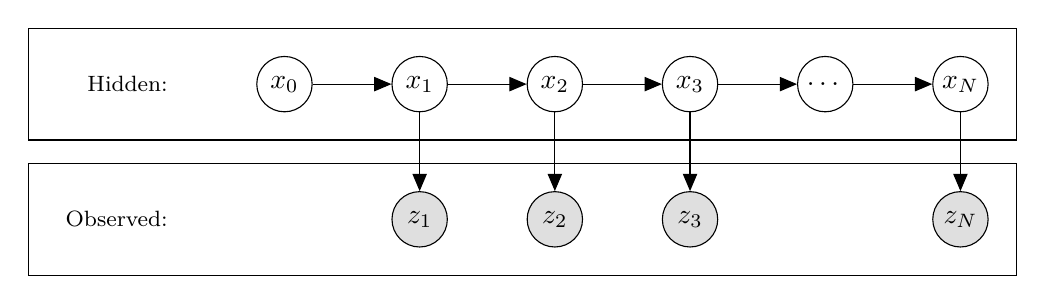
\begin{tikzpicture}
    % States
    \node[latent] (x1) {$\st_1$};
    \node[latent, left=of x1] (x0) {$\st_0$};
    \edge {x0} {x1};
    \node[latent, right=of x1] (x2) {$\st_2$};
    \edge {x1} {x2};
    \node[latent, right=of x2] (x3) {$\st_3$};
    \edge {x2} {x3};
    \node[latent, right=of x3] (x4) {$\dots$};
    \edge {x3} {x4};
    \node[latent, right=of x4] (x5) {$\st_\idxtmax$};
    \edge {x4} {x5};

    % Observations
    \node[obs, below=of x0, draw=none, fill=none] (y0) {};
    \node[obs, below=of x1] (y1) {$\obs_1$};
    \edge {x1} {y1};
    \node[obs, below=of x2] (y2) {$\obs_2$};
    \edge {x2} {y2};
    \node[obs, below=of x3] (y3) {$\obs_3$};
    \edge {x3} {y3};
    \node[obs, below=of x5] (y5) {$\obs_\idxtmax$};
    \edge {x5} {y5};

    \node[rectangle, draw=none, left=of x0] (hidden) {\footnotesize Hidden:};
    \node[rectangle, draw=none, left=of y0] (observed) {\footnotesize Observed:};

    % Observed plate
    \node[rectangle, draw=black, fit={(observed) (y5)}, inner sep=10pt] (observedplate) {};

    % Hidden plate
    \path let \p1 = (observedplate.south west), \p2 = (observedplate.north east) in
    %  node [rectangle, minimum width=\x2-\x1-\pgflinewidth, draw=black, fit={(hidden) (x5)}, inner sep=10pt] (hiddenplate) {};
    %\node[rectangle, above=of observedplate, draw=black] (hiddenplate) {};
      node [rectangle, above=of observedplate, draw=black,
            minimum width=\x2-\x1-\pgflinewidth,
            minimum height=\y2-\y1-\pgflinewidth,
            anchor=center,
            inner sep=10pt] (hiddenplate) {};

  \end{tikzpicture}
  \caption{\textbf{Graphical representation of a Bayesian state-space model.}}
  \label{fig:state-space-model}
\end{figure}

\par
In this chapter, we present recursive and numerically stable algorithms for approximate inference in nonlinear Gaussian state-space models.
\Cref{sec:affine-gaussian-inference} introduces exact Gaussian inference in affine models, and \cref{sec:stable-affine-gaussian-inference} shows how to make this inference numerically stable.
\Cref{sec:lgssm-inference} then presents the recursive algorithm for exact Gaussian inference in linear Gaussian state-space models, commonly known as the Kalman filter and the Rauch--Tung--Striebel smoother.
Then, \cref{sec:nlgssm-inference} shows how to do approximate Gaussian inference in nonlinear models via linearization and develops two recursive algorithms for approximate Gaussian inference in nonlinear Gaussian state-space models.
These will be the main workhorse for the probabilistic numerical methods we develop in later chapters.
\section{Gaussian inference in affine models}
\label{sec:org41b6868}
\label{sec:affine-gaussian-inference}

Consider a Gaussian distribution
\(\p( \st ) = \N( \st; \mean{\st}, \cov{\st} )\)
and a linear Gaussian conditional distribution
\(\p( \obs \mid \st ) = \N( \obs; \transA \st + \transb, \transC )\).
To build Gaussian filtering and smoothing algorithms, we need to perform three basic operations on these distributions:

\begin{enumerate}
\item \textbf{Marginalization:}
The marginal distribution of \(\obs\) is also Gaussian, of the form
\begin{equation}
\p(\obs)
= \int \p(\obs \mid \st) \p(\st) \dd \st
= \N( \obs; \mean{\obs}, \cov{\obs} ),
\end{equation}
with mean and covariance
\begin{subequations}
\begin{align}
\mean{\obs} &= \transA \mean{\st} + \transb, \\
\cov{\obs} &= \transA \cov{\st} \transA^\T + \transC.
\end{align}
\end{subequations}
This is also known as the \emph{prediction} step in Kalman filtering.

\item \textbf{Inversion:}
The conditional distribution of \(\st\) given \(\obs\) is linear Gaussian, of the form
\begin{equation}
\p(\st \mid \obs)
= \frac{\p(\st) \p(\obs \mid \st)}{\p(\obs)}
%= \frac{\p(\st) \p(\obs \mid \st)}{\int \p(\obs \mid \st) \p(\st) \dd \st}
= \N( \st; \invtransA \obs + \invtransb, \invtransC ),
\end{equation}
with parameters
\begin{subequations}\label{eq:gaussian-inversion-parameters}
\begin{align}
\invtransA &= \cov{\st} A^\T \cov{\obs}^{-1}, \\
\invtransb &= \mean{\st} - \invtransA \mean{\obs}, \\
\invtransC &= \cov{\st} - \invtransA \cov{\obs} \invtransA^\T.
\end{align}
\end{subequations}
The covariance \(\Lambda\) can also be computed with equivalent, alternative formulas:
\begin{subequations}
\begin{align}
\invtransC &= (I - \invtransA \transA) \cov{\st}, \\ \text{or} \qquad
\invtransC &= (I - \invtransA \transA) \cov{\st} (I - \invtransA \transA)^\T + \invtransA \transC \invtransA^\T.
\end{align}
\end{subequations}
The latter is also known as the \emph{Joseph form} of the covariance update.

\item \textbf{Update on an observation:}
Given a Gaussian prior \(p(x)\) and linear Gaussian observation model \(p(y \mid x)\) as above, the posterior distribution of \(\st\) given an observation \(\obs=\mathbf{\obs}\) can then be computed by first inverting the observation model, and then evaluating it at the observation, that is
\begin{equation}
\p(\st \mid \obs=\mathbf{\obs})
= \N( \st; \invtransA \mathbf{\obs} + \invtransb, \invtransC ),
\end{equation}
with \(\invtransA\), \(\invtransb\), and \(\invtransC\) as in \cref{eq:gaussian-inversion-parameters}.
This is also known as the \emph{update} step in Kalman filtering.
\end{enumerate}
\section{Numerically stable Gaussian inference in affine models}
\label{sec:orgb087e2e}
\label{sec:stable-affine-gaussian-inference}
When using the formulas presented above
in \cref{sec:affine-gaussian-inference},
the computed covariances can become non-positive semi-definite due to numerical errors.
To avoid these issues we can formulate Gaussian inference in square-root form:
Instead of working with covariance matrices \({\Sigma \in \R^{n \times n}}\),
we work with their square-roots \(\Sigma^{1/2} \in \R^{m \times n}\), defined to satisfy \(\Sigma = (\Sigma^{1/2})^\T \Sigma^{1/2}\).
For example, for positive definite matrices the Cholesky decomposition \(\Sigma = L L^\T\) could provide such a square-root.
But for our purposes we do not require the square-root to be unique and we can work with any square-root of the covariance matrix, including non-square ones (i.e., \(m \neq n\)), as long as they satisfy the relation \(\Sigma = (\Sigma^{1/2})^\T \Sigma^{1/2}\).

For numerically stable Gaussian inference, the formulas that need to be re-derived in square-root form are the computation of the marginal covariance and the covariance of the inverted conditional distribution, namely
\begin{subequations}\label{eq:gaussian-inference-required-cov-operations}
\begin{align}
\cov{\obs} &= \transA \cov{\st} \transA^\T + \transC, \\
\invtransC &= \left( I - \invtransA \transA \right) \cov{\st} \left( I - \invtransA \transA \right)^\T + \invtransA \transC \invtransA^\T.
\end{align}
\end{subequations}
We wrote the latter in the Joseph form to show very clearly that two types of operations are performed on covariance matrices:
multiplication with a matrix from the left and right, and addition of covariance matrices.

\begin{enumerate}
\item \textbf{Multiplication with a matrix from the left and right:}
Given a positive semi-definite matrix \(\Sigma \in \R^{n \times n}\) with square-root \(\Sigma^{1/2} \in \R^{m \times n}\) and some matrix \(A \in \R^{p \times n}\), the product \(A \Sigma A^\T\) satisfies
\begin{equation}
A \Sigma A^\T = A \left( \Sigma^{1/2} \right)^\T \Sigma^{1/2} A^\T = \left( \Sigma^{1/2} A^\T \right)^\T \Sigma^{1/2} A^\T
\end{equation}
Thus, the product can be computed in square-root form with a single matrix-matrix multiplication \(\Sigma^{1/2} A^\T\) without ever forming the full covariance matrix.
\item \textbf{Addition of covariance matrices in square-root form:}
Given two positive semi-definite matrices
\(A \in \R^{n \times n}\) and \(B \in \R^{n \times n}\),
with square-roots
\(A^{1/2} \in \R^{m \times n}\) and \({B^{1/2} \in \R^{p \times n}}\),
a square-root of their sum \(C = A + B\) is given by concatenating the square-roots as
\begin{equation}
C^{1/2} = \begin{bmatrix} A^{1/2} \\ B^{1/2} \end{bmatrix},
\end{equation}
since \((C^{1/2})^\T C^{1/2} = A + B = C\).
Thus, concatenation of square-roots provides a square-root of the sum with minimal computational cost.
But, this approach is impractical when performing many computations on square-root matrices as the resulting matrices would grow in size and become prohibitively large.
To avoid this growth in size, we compress square-root matrices using a QR decomposition.
Given a (possibly non-square) matrix square-root \(A^{1/2} \in \R^{m \times n}\) of some square, positive semi-definite matrix \(A \in \R^{n \times n}\),
we can compute a square matrix square-root \(R \in \R^{n \times n}\) of \(A\) by performing a thin QR decomposition of \(A^{1/2}\), that is
\(Q R = A^{1/2}\),
where \(Q \in \R^{m \times n}\) is an orthogonal matrix and \(R \in \R^{n \times n}\) is an upper triangular matrix.
Then, \(R\) is also a square-root of \(A\), since
\begin{equation}
A = (A^{1/2})^\T A^{1/2} = (Q R)^\T (Q R) = R^\T Q^\T Q R = R^\T R.
\end{equation}
The orthogonal matrix \(Q\) can be discarded after the computation.
We denote this triangularization operation of computing a QR decomposition and returning only \(R\) as \(\tria: \mathbb{R}^{m \times n} \to \mathbb{R}^{n \times n}\).
Thus in summary, computing the sum \(C = A + B\) of two positive semi-definite matrices \(A, B \in \R^{n \times n}\) can be done in square-root form with
\(C^{1/2} = \tria( \smqty[ A^{1/2} \\ B^{1/2} ])\).
\end{enumerate}

Coming back to the required covariance operations in
\cref{eq:gaussian-inference-required-cov-operations},
we can now directly compute
the marginal covariance \(\cov{\obs} = \transA \cov{\st} \transA^\T + \transC\)
and the inverted conditional distribution
\({\invtransC = \left( I - \invtransA \transA \right) \cov{\st} \left( I - \invtransA \transA \right)^\T + \invtransA \transC \invtransA^\T}\)
in square-root form, with
\begin{align}
\label{eq:gaussian-inference-required-cov-operations-sr}
\cov{\obs}^{1/2} = \tria( \mqty[ \transA \cov{\st}^{1/2} \\ \transC^{1/2} ] ),
\qquad
\invtransC^{1/2} = \tria( \mqty[ \cov{\st}^{1/2} (I - \invtransA \transA)^\T \\ \transC^{1/2} \invtransA^\T ] ).
\end{align}
Both terms can be easily verified by multiplying the above expressions with their transposes to recover
\cref{eq:gaussian-inference-required-cov-operations}.
The formulas from
\cref{eq:gaussian-inference-required-cov-operations-sr}
now enable us to perform marginalization, inversion, and update operations in a numerically stable manner.

\begin{alg}[Square-root marginalization in Gaussian affine models]
\algeqspacing
\label{alg:marginalize}
\label{alg:marginalizesr}
Given the parameters
\((\mean{\st}, \cov{\st}^{1/2})\) and
\((\transA, \transb, \transC^{1/2})\)
of distributions
\({\p( \st ) = \N( \st; \mean{\st}, \cov{\st} )}\)
and
\(\p( \obs \mid \st ) = \N( \obs; \transA \st + \transb, \transC )\),
compute the mean and covariance of the Gaussian marginal distribution
\(\p(\obs) = \N( \obs; \mean{\obs}, \cov{\obs} )\)
as
\begin{align}
  \mean{\obs} := \transA \mean{\st} + \transb, \qquad
  \cov{\obs}^{1/2} := \tria( \begin{bmatrix} \transA \cov{\st}^{1/2} \\ \transC^{1/2} \end{bmatrix} ).
\end{align}
Return \(\mean{\obs}, \cov{\obs}^{1/2}\).
\end{alg}

\begin{alg}[Square-root inversion in Gaussian affine models]
\algeqspacing
\label{alg:invert}
\label{alg:invertsr}
Given the parameters
\((\mean{\st}, \cov{\st}^{1/2})\),
\((\transA, \transb, \transC^{1/2})\), and
\((\mean{\obs}, \cov{\obs}^{1/2})\)
of distributions
\({\p( \st ) = \N( \st; \mean{\st}, \cov{\st} )}\),
\(\p( \obs \mid \st ) = \N( \obs; \transA \st + \transb, \transC )\),
and
\(\p( \obs ) = \N( \obs; \mean{\obs}, \cov{\obs} )\),
compute the parameters of the conditional distribution
\(\p(\st \mid \obs) = \N( \st; \invtransA \obs + \invtransb, \invtransC )\)
as
\begin{subequations}
\begin{align}
\invtransA &:= \cov{\st} \transA^\T \cov{\obs}^{-1}, \\
\invtransb &:= \mean{\st} - \invtransA \mean{\obs}, \\
\invtransC^{1/2} &:= \tria( \begin{bmatrix} \cov{\st}^{1/2} (I - \invtransA \transA)^\T \\ \transC^{1/2} \invtransA^\T \end{bmatrix}).
\end{align}
\end{subequations}
Return \(\invtransA, \invtransb, \invtransC^{1/2}\).
\end{alg}

\begin{alg}[Square-root updating on data in Gaussian affine models]
\algeqspacing
\label{alg:update}
\label{alg:updatesr}
Given the parameters
\((\mean{\st}, \cov{\st}^{1/2})\),
\((\transA, \transb, \transC^{1/2})\), and
\((\mean{\obs}, \cov{\obs}^{1/2})\)
of distributions
\({\p( \st ) = \N( \st; \mean{\st}, \cov{\st} )}\),
\(\p( \obs \mid \st ) = \N( \obs; \transA \st + \transb, \transC )\),
and
\(\p( \obs ) = \N( \obs; \mean{\obs}, \cov{\obs} )\),
as well as an observation \(\obs\),
compute the parameters of the posterior distribution of \(\st\) given the observation in two steps:
\begin{enumerate}[nosep]
\item Compute the parameters \((\invtransA, \invtransb, \invtransC^{1/2})\) of the backward transition
\(\p(\st \mid \obs) = \N( \st; \invtransA \obs + \invtransb, \invtransC )\)
with
\cref{alg:invertsr}.
\item Evaluate the backward transition at \(\obs\) to get the posterior mean and covariance:
\begin{subequations}
\begin{align}
\mean{\st} &:= \invtransA \obs + \invtransb, \\
\cov{\st}^{1/2} &:= \invtransC^{1/2}.
\end{align}
\end{subequations}
\end{enumerate}
Return
\(\mean{\st}, \cov{\st}^{1/2}\).
\end{alg}
\section{Sequential inference in linear Gaussian state-space models}
\label{sec:org0834810}
\label{sec:lgssm-inference}
Now that we established the Gaussian inference formulas for affine models, we can derive a general inference algorithm for linear Gaussian state-space models,
which corresponds to the Kalman filter
\parencite{kalman1960}
and the Rauch--Tung--Striebel smoother
\parencite{rauchtungstriebel1965}.
Consider a linear Gaussian state-space model (LGSSM) of the form
\begin{subequations}
\label{eq:lgssm}
\begin{align}
\st_0 &\sim \N( \st_0; \mean{0}, \cov{0} ), \\
\st_\idxt \mid \st_{\idxt-1} &\sim \N( \st_\idxt; \transA_\idxt \st_{\idxt-1} + \transb_\idxt, \transC_\idxt ), \\
\obs_\idxt \mid \st_\idxt &\sim \N( \obs_\idxt; \obsA_\idxt \st_\idxt + \obsb_\idxt, \obsC_\idxt),
\end{align}
\end{subequations}
where
\(\st_\idxt \in \R^{d_\st}\) is the state of the system,
\(\obs_\idxt \in \R^{d_\obs}\) is the observation,
\(\transA_\idxt \in \R^{d_\st \times d_\st}\), \(\transb_\idxt \in \R^{d_\st}\), \(\transC_\idxt \in \R^{d_\st \times d_\st}\)
are the transition model parameters, and
\(\obsA_\idxt \in \R^{d_\obs \times d_\obs}\), \(\obsb_\idxt \in \R^{d_\obs}\), \(\obsC_\idxt \in \R^{d_\obs \times d_\obs}\)
are the observation model parameters
at time \(\idxt\).
Assume also that the square-roots of the covariances are known, i.e., \(\cov{0}^{1/2}\), \(\transC_\idxt^{1/2}\), and \(\obsC_\idxt^{1/2}\) for all \(\idxt = 1, \dots, \idxtmax\).

In the field of Bayesian filtering and smoothing, we are typically interested in computing (some of) the following quantities:
\begin{itemize}[nosep]
\item filtering distributions \(\p(\st_\idxt \mid \obs_{1:\idxt})\) for all \(\idxt\),
\item prediction distributions \(\p(\st_\idxt \mid \obs_{1:\idxt-1})\) for all \(\idxt\),
\item smoothing distributions \(\p(\st_\idxt \mid \obs_{1:N})\) for all \(\idxt\),
\item marginal likelihood \(\p(\obs_{1:N})\),
\item the full posterior \(\p(\st_{0:N} \mid \obs_{1:N})\); since it satisfies
\begin{equation}
\p(\st_{0:N} \mid \obs_{1:N})
  %= \p(\st_{N} \mid \obs_{1:N}) \prod_{\idxt=0}^{N-1} \p(\st_\idxt \mid \st_{\idxt+1}, \obs_{1:N})
  = \p(\st_{N} \mid \obs_{1:N}) \prod_{\idxt=0}^{N-1} \p(\st_\idxt \mid \st_{\idxt+1}, \obs_{1:\idxt}),
\end{equation}
it is sufficient to compute the filtering distribution \(\p(\st_{N} \mid \obs_{1:N})\) and the backwards transitions \(\{\p(\st_\idxt \mid \st_{\idxt+1}, \obs_{1:\idxt})\}_{\idxt=0}^{N-1}\).
\end{itemize}

It turns out that all of these quantities can be computed recursively
by applying the Gaussian inference formulas from
\cref{sec:affine-gaussian-inference,sec:stable-affine-gaussian-inference}.

\begin{alg}[Inference in affine Gaussian state-space models]
\algeqspacing
\label{alg:lgssm-inference}
Given the parameters of an LGSSM
\((\mean{0}, \cov{0}^{1/2}), (\transA_{1:N}, \transb_{1:N}, \transC_{1:N}^{1/2}), (\obsA_{1:N}, \obsb_{1:N}, \obsC_{1:N}^{1/2})\)
(as in Equation \ref{eq:lgssm})
and a sequence of observations \(\obs_{1:N}\),
perform sequential Gaussian inference in the LGSSM:
\begin{enumerate}[nosep]
\item Initialize the log-likelihood, defined as \(\text{LL}_\idxt := \p(\obs_{1:\idxt})\), with
\(\text{LL}_0 = 0\).
\item For \(\idxt = 1, \dots, N\) do
\begin{itemize}
\item \textbf{Predict:} Compute
\(\p(\st_\idxt \mid \obs_{1:\idxt-1}) = \N( \st_\idxt; \mean{\idxt}^P, \cov{\idxt}^P )\)
with
\begin{fleqn}
\begin{equation*}
  \mean{\idxt}^P, \cov{\idxt}^P := \operatorname{MARGINALIZE}\left(
    (\mean{{\idxt-1}}, \cov{{\idxt-1}}),
    (\transA_\idxt, \transb_\idxt, \transC_\idxt)
  \right).
  \tag{\cref{alg:marginalize}}
\end{equation*}
\end{fleqn}
\item \textbf{Compute the observation estimate:}
\(\p(\obs_\idxt \mid \obs_{1:\idxt-1}) = \N( \obs_\idxt; \hat{\obs}_\idxt, S_\idxt )\)
with
\begin{fleqn}
\begin{equation*}
  \hat{\obs}_\idxt, S_\idxt := \operatorname{MARGINALIZE}\left(
    (\mean{\idxt}^P, \cov{\idxt}^P),
    (\obsA_\idxt, \obsb_\idxt, \obsC_\idxt)
  \right).
  \tag{\cref{alg:marginalize}}
\end{equation*}
\end{fleqn}
\item \textbf{Increment the log-likelihood}
\begin{fleqn}
\begin{equation*}
 \text{LL}_\idxt := \text{LL}_{\idxt-1} + \log \N( \obs_\idxt; \hat{\obs}_\idxt, S_\idxt ).
\end{equation*}
\end{fleqn}
\item \textbf{Update:} Compute
\(\p(\st_\idxt \mid \obs_{1:\idxt}) = \N( \st_\idxt; \mean{\idxt}, \cov{\idxt} )\)
with
\begin{fleqn}
\begin{equation*}
  \mean{\idxt}, \cov{\idxt} := \operatorname{UPDATE}\left(
    (\mean{\idxt}^P, \cov{\idxt}^P),
    (\obsA_\idxt, \obsb_\idxt, \obsC_\idxt),
    (\hat{\obs}_\idxt, S_\idxt),
    \obs_\idxt
  \right).
  \tag{\cref{alg:update}}
\end{equation*}
\end{fleqn}
\item (Optional) \textbf{Compute the backward transition}
\(\p(\st_{\idxt-1} \mid \st_\idxt, \obs_{1:\idxt-1}) = \N( \st_{\idxt-1}; \invtransA_\idxt \st_\idxt + \invtransb_\idxt, \invtransC_\idxt )\) with
\begin{fleqn}
\begin{equation*}
  \invtransA_\idxt, \invtransb_\idxt, \invtransC_\idxt := \operatorname{INVERT} \left(
    (\mean{{\idxt-1}}, \cov{{\idxt-1}}),
    (\mean{\idxt}^P, \cov{\idxt}^P),
    (\transA_\idxt, \transb_\idxt, \transC_\idxt)
  \right).
  \tag{\cref{alg:invert}}
\end{equation*}
\end{fleqn}
\end{itemize}
\item (Optional) \textbf{Compute the posterior marginals}
\begin{itemize}
\item Set \(\mean{N}^S, \cov{N}^S := \mean{N}, \cov{N}\)
\item For \(\idxt = N, \dots, 1\) compute
\begin{equation*}
  \mean{{\idxt-1}}^S, \cov{{\idxt-1}}^S := \operatorname{MARGINALIZE}\left(
    (\mean{\idxt}^S, \cov{\idxt}^S),
    (\invtransA_\idxt, \invtransb_\idxt, \invtransC_\idxt)
  \right)
  \tag{\cref{alg:marginalize}}
\end{equation*}
\end{itemize}
\end{enumerate}
Return the parameters of all desired quantities:
\begin{itemize}[nosep]
\item the filtering distributions: \((\mean{{1:N}}, \cov{{1:N}})\),
\item the smoothing distributions: \((\mean{{1:N}}^S, \cov{{1:N}}^S)\),
\item the log-likelihood: \(\text{LL}_N\),
\item the backward transitions of the posterior: \((\invtransA_{1:N}, \invtransb_{1:N}, \invtransC_{1:N})\).
\end{itemize}
\end{alg}

If we only compute the filtering distributions, \cref{alg:lgssm-inference} corresponds exactly to a (square-root) Kalman filter.
Similarly, the smoothing distributions returned by this algorithm correspond exactly to those returned by a (square-root) Rauch--Tung--Striebel smoother.
The sequential likelihood computation is also known as prediction error decomposition
\parencite{schweppe1965evaluation}.

\begin{remark}[Missing observations]
If for certain time steps \(\idxt\) the observation \(\obs_\idxt\) is missing, \cref{alg:lgssm-inference} can still be used for exact inference by simply skipping the observation estimate computation, the log-likelihood increment, and the update step for these steps.
\end{remark}

\begin{remark}[On the computational (in)efficiency of \cref{alg:lgssm-inference}]
Our presentation of \cref{alg:lgssm-inference} favors simplicity over efficiency:
By sticking to the simple building blocks of Gaussian marginalization, inversion, and updating,
we aim to formulate Gaussian filtering and smoothing in a very simple and intuitive manner.
This hopefully empowers the reader to approach more complex state-estimation problems and build custom algorithms for these, by simply reducing the required steps to the three building blocks.
On the flip side, the strict separation into these building blocks leads to some redundant computations and therefore to suboptimal performance.
But this can easily be improved in an actual implementation by merging some of these operations.
\end{remark}
\subsection{Example: Sequential inference in a simple LGSSM}
\label{sec:org9c5fe89}
\label{example:lgssm-inference}

To give a brief example, we apply the LGSSM inference algorithm (\ref{alg:lgssm-inference})
to a simple Bayesian state estimation problem.
We consider an LGSSM given by
\begin{subequations}
\begin{align}
\st_0 &\sim \N( \st_0; \mqty[0\\0], \mqty[\dmat{ 1, 1}]), \\
\st_\idxt \mid \st_{\idxt-1} &\sim \N(
  \st_\idxt;
  \mqty[1 & \dt \\ & 1] \st_{\idxt-1},
  \mqty[\frac{\dt^3}{3} & \frac{\dt^2}{2} \\ \frac{\dt^2}{2^{}} & \dt]
), \\
\obs_\idxt \mid \st_\idxt &\sim \N( \obs_\idxt; \mqty[1&0] \st_\idxt, 0.25),
\end{align}
\end{subequations}
with \(\dt = \frac{4\pi}{100}\); this parameter can be interpreted as the step size at which some underlying continuous model is discretized.
We generate synthetic data as noisy draws from a sine function
\(\obs_\idxt = \sin(\idxt \cdot \dt) + \varepsilon_\idxt\) with \(\varepsilon_\idxt \sim \N( \varepsilon_\idxt; 0, 0.25)\) for \(\idxt = 1, \dots, 100\).
We then perform inference with the LGSSM inference algorithm (\ref{alg:lgssm-inference}).

\begin{figure}[t]
\centering
\includegraphics[width=\textwidth]{./figures/kalmanfilterexample.pdf}
\caption{\label{fig:kalmanfilterexample}\textbf{Filtering and smoothing outputs for an LGSSM inference problem.} The filtering distribution appears closer to the observations, but the smoothing distribution is a better estimate for the underlying function of interest (black dashed line). Sampling from the posterior gives the most expressive description as it also visualizes temporal correlations.}
\end{figure}

\Cref{fig:kalmanfilterexample}
visualizes the quantities returned by the method, projected into the observation space via multiplication with the observation matrix \(H=\mqty[1&0]\).
The filtering distribution often appears to be closer to the observations, but it is very non-smooth.
The smoothing distribution is in comparison a much better estimate for the true solution trajectory as it is able to take into account all data,
but it also shows only marginal distributions.
Sampling from the posterior distribution returned by the method gives the most expressive description here as it also visualizes temporal correlations.
\section{Sequential approximate inference in nonlinear Gaussian state-space models}
\label{sec:orgba2d3eb}
\label{sec:nlgssm-inference}
The state-space models that we are ultimately interested in are unfortunately not linear.
But, we can still build on the LGSSM inference algorithm from the previous section.
We consider a nonlinear Gaussian state-space model (NLGSSM) of the form
\begin{subequations}
\label{eq:nlgssm}
\begin{align}
\st_0 &\sim \N( \st_0; \mean{0}, \cov{0} ), \\
\st_\idxt \mid \st_{\idxt-1} &\sim \N( \st_\idxt; \transf_\idxt(\st_{\idxt-1}), \transC_\idxt ), \\
\obs_\idxt \mid \st_\idxt &\sim \N( \obs_\idxt; \obsh_\idxt(\st_\idxt), \obsC_\idxt),
\end{align}
\end{subequations}
where
\(\st_\idxt \in \R^{d_\st}\) is the state,
\(\obs_\idxt \in \R^{d_\obs}\) is the observation,
\(\transf_\idxt : \R^{d_\st} \to \R^{d_\st}\) is a nonlinear transition function,
\(\obsh_\idxt : \R^{d_\st} \to \R^{d_\obs}\) is a nonlinear observation function,
and \(\transC_\idxt \in \R^{d_\st \times d_\st}\), \(\obsC_\idxt \in \R^{d_\obs \times d_\obs}\) are noise covariances
at time \(\idxt = 1, \dots, \idxtmax\).
As before, we assume that the covariances are known in square-root form, i.e., \(\cov{0}^{1/2}\), \(\transC_\idxt^{1/2}\), and \(\obsC_\idxt^{1/2}\).
\subsection{Linearizing conditional Gaussian distributions}
\label{sec:org4ca1fc6}
\label{sec:linearization}
In nonlinear models the marginal distribution, the inverse transition, and the updated distribution all become non-Gaussian,
and the three building blocks that we defined in
\cref{sec:affine-gaussian-inference,sec:stable-affine-gaussian-inference}
are not directly applicable.
One conceptually simple approach for developing efficient, approximate inference algorithms is via linearization:
By approximating the nonlinear conditional Gaussian distributions into affine models, we can build on the Gaussian inference framework that we established so far to perform efficient, closed-form inference.

The linearization step can be performed in different ways, and many approaches for linearizing conditional Gaussian distributions have been proposed in the filtering and smoothing literature.
We will focus on linearization via Taylor-approximation here as it is conceptually simple, very well-known, efficient, and tends to work well in practice.

To this end, consider a Gaussian distribution
\(\p(\st) = \N( \st; \mean{\st}, \cov{\st} )\)
with mean \(\mean{\st} \in \R^N\) and covariance \(\cov{\st} \in \R^{N \times N}\)
and a nonlinear Gaussian observation model
\(\p(\obs \mid \st) = \N( \obs; \obsh(\st), R )\),
where \(h: \R^n \to \R^m\) is a nonlinear function.
By doing a first-order Taylor expansion of \(\obsh\) around some point \(\xi \in \R^n\), we obtain
\begin{equation}
  % \obsh(\st) \approx \bar{h}_\xi(\st) := \obsh(\xi) + \jac{\obsh}(\xi) (\st - \xi),
  \obsh(\st) = \underbrace{\obsh(\xi) + \jac{\obsh}(\xi) (\st - \xi)}_{=: \bar{\obsh}_\xi(\st)} + \order{\| \st - \xi \|},
\end{equation}
where \(\jac{\obsh}(\xi) \in \R^{m \times n}\) is the Jacobian of \(\obsh\) at \(\xi\).
Then, we approximate \(\obsh\) with \(\bar{h}_\xi\) to obtain a new, \emph{affine} approximate observation model
\(\q(\obs \mid \st) \approx \p(\obs \mid \st)\),
with which we can then apply all the Gaussian inference algorithms from
\cref{sec:affine-gaussian-inference,sec:stable-affine-gaussian-inference}
to perform approximate inference.
We summarize the linearization approach in the following algorithm.

\begin{alg}[Linearization via Taylor-approximation]
\algeqspacing
\label{alg:linearize}
Given the parameters \((\obsh, \obsC)\) of a nonlinear conditional Gaussian distribution
\(\p(\obs \mid \st) = \N( \obs; \obsh(\st), \obsC )\),
and a linearization point \(\xi \in \R^n\),
compute the Gaussian approximation
\(\q(\obs \mid \st) = \N( \obs; \obsA \st + \obsb, \obsC )\)
with
\begin{subequations}
\begin{align}
  \obsA &:= \jac{h}(\xi), \\
  \obsb &:= \obsh(\xi) - \obsA \xi,
\end{align}
\end{subequations}
Return the parameters
\((\obsA, \obsb, \obsC)\)
of the linearized model.
\end{alg}

This is exactly the approach taken in the extended Kalman filter and extended Rauch--Tung--Striebel smoother: By linearizing the observation model in this way, the problem becomes affine and inference becomes tractable.
We did not yet discuss how to select the linearization point \(\xi\),
but we will discuss two common approaches in the next sections which lead to two different algorithms:
local linearization at the predicted mean, and
iterated posterior linearization.

\begin{remark}[Alternative linearization approaches]
There are many other ways to linearize a nonlinear Gaussian model, for example with
higher-order Taylor approximations,
quadrature-based methods (e.g. Gauss--Hermite cubature, spherical cubature, the unscented transform, \ldots{}),
statistical linearization,
or statistical linear regression
(which can even be applied to non-Gaussian models).
For a more detailed discussion of these methods, refer to
\textcite[Chapter 7-10]{Särkkä_Svensson_2023}.
\end{remark}
\subsection{Local linearization: The extended Kalman filter and smoother}
\label{sec:org78085c2}
\label{sec:local-linearization}
\label{sec:nlgssm-inference:local}

One common choice for the linearization point is the prior mean, that is \(\xi = \mean{x}\).
To apply this to the NLGSSM inference problem from \cref{eq:nlgssm},
this means that we always linearize the transition and observation models around the mean of the ``current best'' state estimate:
at each step, we linearize the transition model around the filtering mean
such that we can then predict the next state with the linearized model,
and we linearize the observation model around the predicted mean before computing the likelihood and updating the state.
The resulting algorithm is also known as the (square-root) extended Kalman filter and (square-root) extended Rauch--Tung--Striebel smoother, and we summarize it in the following algorithm.

\begin{alg}[Approximate inference in nonlinear Gaussian state-space models]
\setlength{\belowdisplayskip}{3pt}
\setlength{\belowdisplayshortskip}{2pt}
\setlength{\abovedisplayskip}{3pt}
\setlength{\abovedisplayshortskip}{-8pt}
\label{alg:nlgssm-inference}
\label{alg:nlgssm-inference:local}
Given the parameters of an NLGSSM
\((\mean{0}, \cov{0}^{1/2}), (\transf_{1:N}, \transC_{1:N}^{1/2}), (\obsh_{1:N}, \obsC_{1:N}^{1/2})\),
as in \cref{eq:lgssm},
and a sequence of observations \(\obs_{1:N}\),
perform sequential Gaussian inference in the LGSSM:
\begin{enumerate}[nosep]
\item Initialize the log-likelihood \(\text{LL}_0 = 0\)
\item For \(\idxt = 1, \dots, N\) do
\begin{itemize}
\item \textbf{Linearize the transition model:}
\begin{fleqn}
\begin{equation*}
  \transA_\idxt, \transb_\idxt, \transC_\idxt := \operatorname{LINEARIZE}\left(
    \transf_\idxt, \transC_\idxt^{1/2}, \mean{{\idxt-1}},
  \right),
  \tag{\cref{alg:linearize}}
\end{equation*}
\end{fleqn}
\item \textbf{Predict:} Compute
\(\p(\st_\idxt \mid \obs_{1:\idxt-1}) = \N( \st_\idxt; \mean{\idxt}^P, \cov{\idxt}^P )\) with
\begin{fleqn}
\begin{equation}
  \mean{\idxt}^P, \cov{\idxt}^P := \operatorname{MARGINALIZE}\left(
    (\mean{{\idxt-1}}, \cov{{\idxt-1}}),
    (\transA_\idxt, \transb_\idxt, \transC_\idxt)
  \right).
  \tag{\cref{alg:marginalize}}
\end{equation}
\end{fleqn}
\item \textbf{Linearize the observation model:}
\begin{fleqn}
\begin{equation*}
 \obsA_\idxt, \obsb_\idxt, \obsC_\idxt := \operatorname{LINEARIZE}\left(
   \obsh_\idxt, \obsC_\idxt^{1/2}, \mean{\idxt}^P,
  \right),
  \tag{\cref{alg:linearize}}
\end{equation*}
\end{fleqn}
\item \textbf{Compute observation estimate:}
\(\p(\obs_\idxt \mid \obs_{1:\idxt-1}) = \N( \obs_\idxt; \hat{\obs}_\idxt, S_\idxt )\)
with
\begin{fleqn}
\begin{equation}
  \hat{\obs}_\idxt, S_\idxt := \operatorname{MARGINALIZE}\left(
    (\mean{\idxt}^P, \cov{\idxt}^P),
    (\obsA_\idxt, \obsb_\idxt, \obsC_\idxt)
  \right).
  \tag{\cref{alg:marginalize}}
\end{equation}
\end{fleqn}
\item \textbf{Increment the log-likelihood}
\begin{fleqn}
\begin{equation*}
 \text{LL}_\idxt := \text{LL}_{\idxt-1} + \log \N( \obs_\idxt; \hat{\obs}_\idxt, S_\idxt ).
\end{equation*}
\end{fleqn}
\item \textbf{Update:} Compute
\(\p(\st_\idxt \mid \obs_{1:\idxt}) = \N( \st_\idxt; \mean{\idxt}, \cov{\idxt} )\)
with
\begin{fleqn}
\begin{equation}
  \mean{\idxt}, \cov{\idxt} := \operatorname{UPDATE}\left(
    (\mean{\idxt}^P, \cov{\idxt}^P),
    (\obsA_\idxt, \obsb_\idxt, \obsC_\idxt),
    (\hat{\obs}_\idxt, S_\idxt),
    \obs_\idxt
  \right).
  \tag{\cref{alg:update}}
\end{equation}
\end{fleqn}
\item (Optional) \textbf{Compute the backward transition}
\(\p(\st_{\idxt-1} \mid \st_\idxt, \obs_{1:\idxt-1}) = \N( \st_{\idxt-1}; \invtransA_\idxt \st_\idxt + \invtransb_\idxt, \invtransC_\idxt )\) with
\begin{fleqn}
\begin{equation}
  \invtransA_\idxt, \invtransb_\idxt, \invtransC_\idxt := \operatorname{INVERT} \left(
    (\mean{{\idxt-1}}, \cov{{\idxt-1}}),
    (\mean{\idxt}^P, \cov{\idxt}^P),
    (\transA_\idxt, \transb_\idxt, \transC_\idxt)
  \right)
  \tag{\cref{alg:invert}}
\end{equation}
\end{fleqn}
\end{itemize}
\item (Optional) \textbf{Compute the posterior marginals}
\begin{itemize}
\item Set \(\mean{N}^S, \cov{N}^S := \mean{N}, \cov{N}\)
\item For \(\idxt = N, \dots, 1\) compute
\begin{fleqn}
\begin{equation}
  \mean{{\idxt-1}}^S, \cov{{\idxt-1}}^S := \operatorname{MARGINALIZE}\left(
    (\mean{\idxt}^S, \cov{\idxt}^S),
    (\invtransA_\idxt, \invtransb_\idxt, \invtransC_\idxt)
  \right)
  \tag{\cref{alg:marginalize}}
\end{equation}
\end{fleqn}
\end{itemize}
\end{enumerate}
Return the parameters of all desired quantities:
\begin{itemize}[nosep]
\item the filtering distributions: \((\mean{{1:N}}, \cov{{1:N}})\),
\item the smoothing distributions: \((\mean{{1:N}}^S, \cov{{1:N}}^S)\),
\item the log-likelihood: \(\text{LL}_N\),
\item the backward transitions of the posterior: \((\invtransA_{1:N}, \invtransb_{1:N}, \invtransC_{1:N})\).
\end{itemize}
\end{alg}
\begin{remark}[On affine models, \cref{alg:nlgssm-inference:local} is equivalent to \cref{alg:lgssm-inference} and performs exact inference]
First-order Taylor approximations of affine functions are exact.
Therefore, given a model with affine transition and observation functions, the general NLGSSM inference algorithm \ref{alg:nlgssm-inference:local} returns the same result as the LGSSM inference algorithm \ref{alg:lgssm-inference} and thus performs exact inference.
\end{remark}
\subsection{Global linearization: The iterated extended Kalman smoother}
\label{sec:org80e6674}
\label{sec:iterated-linearization}
\label{sec:nlgssm-inference:global}

Instead of linearizing the NLGSSM at each time step separately, we can also linearize the entire model \emph{globally} over some trajectory of linearization points \(\xi_{1:\idxtmax}\).
This is done in the \emph{iterated extended Kalman smoother} (IEKS):
Given an initial trajectory of linearization points \(\xi_{1:\idxtmax}\),
the IEKS linearizes the entire model around these points and then performs a single pass of the Kalman smoother to compute the posterior.
Then, the mean of the posterior marginals is used as the new linearization points, and the process is repeated until convergence.

\begin{alg}[Iterated extended Kalman smoother]
\setlength{\belowdisplayskip}{3pt}
\setlength{\belowdisplayshortskip}{2pt}
\setlength{\abovedisplayskip}{3pt}
\setlength{\abovedisplayshortskip}{-8pt}
\label{alg:ieks}
\label{alg:nlgssm-inference:global}
Given the parameters of an NLGSSM as in \cref{eq:lgssm}
\((\mean{0}, \cov{0}^{1/2}), (\transf_{1:N}, \transC_{1:N}^{1/2}), (\obsh_{1:N}, \obsC_{1:N}^{1/2})\),
a sequence of observations \(\obs_{1:N}\),
and an initial trajectory of linearization points \(\xi_{0:N}\),
repeat the following steps until convergence:
\begin{enumerate}[nosep]
\item Linearize the entire model around the linearization points for all \(\idxt = 1, \dots, N\):
\begin{align*}
  \transA_\idxt, \transb_\idxt, \transC_\idxt &:= \operatorname{LINEARIZE}\left(
    \transf_\idxt, \transC_\idxt^{1/2}, \xi_{\idxt-1}
  \right),
  \tag{\cref{alg:linearize}}\\
  \obsA_\idxt, \obsb_\idxt, \obsC_\idxt &:= \operatorname{LINEARIZE}\left(
    \obsh_\idxt, \obsC_\idxt^{1/2}, \xi_\idxt
  \right).
   \tag{\cref{alg:linearize}}
\end{align*}
\item Compute the posterior marginals of the linearized LGSSM with \cref{alg:lgssm-inference}:
\begin{equation*}
  \begin{split}
  (\mean{{0:N}}^S , \cov{{0:N}}^S), & \ldots := \operatorname{LGSSM\_INFERENCE}\big(\\
    &(\mean{0}, \cov{0}^{1/2}), (\transA_{1:N}, \transb_{1:N}, \transC_{1:N}), (\obsA_{1:N}, \obsb_{1:N}, \obsC_{1:N}), \obs_{1:N}
  \big)
  \end{split}
  % \tag{\cref{alg:lgssm-inference}}
\end{equation*}
\item Set the new linearization points to the posterior means:
\(\xi_\idxt := \mean{\idxt}^S\) for all \(\idxt\).
\end{enumerate}
Return the parameters of all desired quantities:
the smoothing distributions \((\mean{{1:N}}^S, \cov{{1:N}}^S)\), the posterior, the log-likelihood, \ldots{}
\end{alg}

The IEKS is a powerful method which often leads to good results in nonlinear models \parencite{Särkkä_Svensson_2023}.
It is also known to (locally) converge to the maximum a posteriori (MAP) estimate of the state trajectory.
That is, the returned posterior means satisfy (in the limit)
\begin{equation}
  \label{eq:map-estimate}
  \mean{{1:N}}^S = \argmax_{\st_{1:N}} \p(\st_{1:N} \mid \obs_{1:N}).
\end{equation}
The IEKS algorithm is also known to be equivalent to the Gauss--Newton method for computing this MAP estimate, implemented in a recursive, sequential manner;
refer to \textcite{Bell1994} for a detailed discussion of this connection.
Finally, the initial trajectory of linearization points \(\xi_{1:N}\) is typically computed with a local-linearization-based extended Kalman smoother (\cref{alg:nlgssm-inference:local}).
This can help speed up the convergence of the IEKS if the initial trajectory is already close to the MAP estimate.
But overall, the IEKS comes with a larger computational cost than its non-iterated counterpart.
\subsection{Example: Sequential inference in an NLGSSM}
\label{sec:orga1d0759}
We demonstrate both NLGSSM inference algorithms
\ref{alg:nlgssm-inference:local}
and
\ref{alg:nlgssm-inference:global}
on a simple but nonlinear Bayesian state estimation problem.
Consider the NLGSSM given by
\begin{subequations}
\begin{align}
\st_0 &\sim \N( \st_0; \mqty[0\\0], \mqty[\dmat{ 1, 1}]), \\
\st_{\idxt+1} \mid \st_\idxt &\sim \N(
  \st_{\idxt+1};
  \mqty[(\st_\idxt)_1 + (\st_\idxt)_2 \dt \\ (\st_\idxt)_2 - 9.81 \sin((\st_\idxt)_1) \dt],
  \mqty[\frac{\dt^3}{3} & \frac{\dt^2}{2} \\ \frac{\dt^2}{2^{}} & \dt]
), \\
\obs_\idxt \mid \st_\idxt &\sim \N( \obs_\idxt; \sin(\mqty[1&0] \st_\idxt), 0.3^2),
\end{align}
\end{subequations}
with \(\dt = 1/80\); this parameter can be interpreted as the step size at which some underlying continuous model is discretized.
We generate ground-truth states and observations by sampling from this NLGSSM for \(\idxt = 0, \dots, 400\), starting with a known \(\st_0=\mqty[\pi/2 & 0]^\T\).
Then, we infer the unknown states \(\st_{0:400}\) from the observations \(\obs_{0:400}\) with both the local-linearization-based NLGSSM inference algorithm \ref{alg:nlgssm-inference} (\texttt{EKS})
and with the iterated global linearization-based algorithm \ref{alg:nlgssm-inference:global} (\texttt{IEKS}).

\begin{figure}[t]
\centering
\includegraphics[width=\textwidth]{./figures/nlgssmexample.pdf}
\caption{\label{fig:nlgssmexample}\textbf{NLGSSM inference results with the local and iterated global linearization.} \emph{Left}: The problem setting, consisting of a true underlying function and nonlinear observations. \emph{Center}: The local-linearization-based \texttt{EKS} is able to return an accurate and calibrated estimate. \emph{Right}: The iterated, global linearization-based \texttt{IEKS} also returns an accurate and calibrated estimate, but in particular in the beginning of the time interval the estimate is more accurate and more certain than the \texttt{EKS}.}
\end{figure}

\Cref{fig:nlgssmexample} shows the results.
Overall we observe that both methods return meaningful posterior estimates for the true underlying state, with both accurate mean estimates and good coverage by the \(95\%\) credible intervals.
The difference between the \texttt{EKS} and the \texttt{IEKS} appears most prominently in the very beginning of the trajectory:
the \texttt{EKS} is calibrated but rather uncertain about the initial value,
whereas the \texttt{IEKS} is able to estimate the true initial value with both high accuracy and low uncertainty.
We can also evaluate the quality of the posterior mean by computing its root mean square error (RMSE) with respect to the true trajectory, defined as
\begin{equation}
  \operatorname{RMSE}(\mean{1:N}) = \sqrt{\frac{1}{N} \sum_{\idxt=1}^N \| \mean{\idxt}  - \st_\idxt^{\text{(true)}} \|_2^2}.
\end{equation}
We obtain RMSEs of \(0.52\) for the \texttt{EKS} and \(0.48\) for the \texttt{IEKS},
indicating again that while both methods returned similar results on this simple example, the \texttt{IEKS} tends to be a bit more accurate.
This difference can be much more pronounced on more complicated problems, and the MAP estimate computed by the \texttt{IEKS} is often the more accurate (as well as more interpretable) result.
For more examples and a much more thorough discussion, refer to
\textcite{Särkkä_Svensson_2023}.
\section{\wrapupsec{}}
\label{sec:org27bf838}
In this chapter, we introduced linear and nonlinear Gaussian state-space models and developed efficient algorithms for exact and approximate inference.
At their core, these methods all build on three building blocks of Gaussian inference: marginalization, inversion, and updating on an observation.
From these, we derived the sequential inference algorithm for linear Gaussian state-space models, known as the Kalman filter and Rauch--Tung--Striebel smoother.
For nonlinear models, we simply linearize the nonlinearities via Taylor-approximation and then again rely on the Gaussian inference formulas.
When done locally we obtain the extended Kalman filter and extended Rauch--Tung--Striebel smoother, and when iterated globally we obtain the iterated extended Kalman smoother.
These inference algorithms will be the main workhorse of the probabilistic numerical ODE solvers developed in later chapters.
\chapter{Gauss--Markov Processes}
\label{sec:org462d373}
\label{sec:gauss-markov-processes}

This chapter considers problems of estimating unknown \emph{functions} from observations.
\Cref{sec:gps} introduces
\emph{Gaussian processes} (GPs), a general framework for modeling and inferring unknown functions that is well-known in machine learning.
But, their computational cost can be prohibitive for certain applications as it scales cubically with the number of data points---which would be particularly problematic for our application of simulating ODEs as the number of steps performed by numerical solvers can become arbitrarily large.
To address this issue,
\cref{sec:lti-sdes} introduces a different framework for working with certain Gaussian processes,
namely linear time-invariant stochastic differential equations,
and shows how we can work with the resulting Gauss--Markov processes in a computationally efficient manner with recursive algorithms and with linear cost \(\order{N}\).
This is explained in \cref{sec:gauss-markov-process-regression}.
\Cref{sec:nonlinear-gmp-regression} then extends this framework to nonlinear observation models and provides efficient approximate inference procedures.
\section{Gaussian process regression}
\label{sec:org0bffd9b}
\label{sec:gps}
\label{sec:gp-regression}

Gaussian processes provide a convenient framework for modeling and inferring unknown functions.
We follow
\textcite[Definition 2.1]{rasmussen2005gpml}
and define them in the following way.

\begin{definition}[Gaussian Process]
A \emph{Gaussian process} (GP) is a collection of random variables on a common space \(\mathbb{R}^\numdims\), any finite number of which have a joint Gaussian distribution.
\end{definition}

A Gaussian process \(\sval\) is typically described by its mean function \(\gpmeanfun\) and its covariance function \(\gpcovfun\) (or \emph{kernel function}) as
\begin{subequations}
\begin{align}
\gpmeanfun(\xi) &= \mathbb{E}\left[ \sval(\xi) \right], \\
\gpcovfun(\xi, \xi') &= \mathbb{E}\left[
    \left(\sval(\xi) - \gpmeanfun(\xi)\right)
    \left(\sval(\xi') - \gpmeanfun(\xi')\right)^\T
  \right],
\end{align}
\end{subequations}
and we write \(\sval \sim \GP( \gpmeanfun, \gpcovfun )\).
Given a finite collection of inputs \(\{\xi_\idxt\}_{\idxt=1}^\idxtmax\), the function values \(\{\sval(\xi_\idxt)\}_{\idxt=1}^\idxtmax\) are jointly Gaussian distributed, as
\begin{equation}
\mqty(\sval(\xi_1) \\ \vdots \\ \sval(\xi_\idxtmax))
\sim \N(\mqty(\gpmeanfun(\xi_1) \\ \vdots \\ \gpmeanfun(\xi_\idxtmax)),
      \mqty(
        \gpcovfun(\xi_1, \xi_1) & \cdots & \gpcovfun(\xi_1, \xi_\idxtmax) \\
        \vdots & \ddots & \vdots \\
        \gpcovfun(\xi_\idxtmax, \xi_1) & \cdots & \gpcovfun(\xi_\idxtmax, \xi_\idxtmax)
      )).
\end{equation}
More compactly, we denote collections of inputs using subscripts, i.e. \(\xi_{1:\idxtmax}\), and with a slight abuse of notation we write
\begin{equation}
\sval(\xi_{1:\idxtmax}) \sim \N( \gpmeanfun(\xi_{1:\idxtmax}), \gpcovfun(\xi_{1:\idxtmax}, \xi_{1:\idxtmax}) ).
\end{equation}
The covariance matrix \(\gpcovfun(\xi_{1:\idxtmax}, \xi_{1:\idxtmax})\) is also referred to as the \emph{kernel matrix} or \emph{Gram matrix}.
Without loss of generality we only consider zero-mean Gaussian processes with \(\gpmeanfun \equiv 0\)
\parencite{rasmussen2005gpml}.

\begin{figure}[t]
\centering
\includegraphics[width=\textwidth]{./figures/gp_priors.pdf}
\caption{\label{fig:gp_priors}\textbf{Examples of various Gaussian process priors.} Samples (top) and kernel matrix (bottom) for a range of different priors (columns).}
\end{figure}

\begin{exmple}[Popular GP kernels]
\label{example:gp-kernels}
Popular covariance functions used for GP regression include:
\begin{enumerate}
\item \emph{Wiener process}:
\begin{equation}
\gpcovfun_\text{Wiener}(\xi, \xi') = \sigma^2 \min(\xi, \xi'),
\end{equation}
for one-dimensional non-negative \(\xi \in \R_{\geq0}\), with a scale hyperparameter \(\sigma^2\).
\item \emph{Wiener velocity}:
\begin{equation}
\gpcovfun_\text{WienerVel}(\xi, \xi') = \sigma^2 \left(
  \frac{\min^3(\xi, \xi')}{3} + \abs{\xi - \xi'} \frac{\min^2(\xi, \xi')}{2}
\right)
\end{equation}
for one-dimensional non-negative \(\xi \in \R_{\geq0}\), with a scale hyperparameter \(\sigma^2\).
\item \emph{Matérn}:
\begin{equation}
\gpcovfun_\text{Mat\'ern}(\xi, \xi') = \sigma^2 \frac{2^{1-\nu}}{\Gamma(\nu)} \left( \frac{\sqrt{2\nu}}{\ell} \norm{\xi - \xi'} \right)^\nu K_\nu\left( \frac{\sqrt{2\nu}}{\ell} \norm{\xi - \xi'} \right),
\end{equation}
where \(\sigma^2\) is a scale hyperparameter, \(\ell\) is a lengthscale hyperparameter, and \(\nu\) is a smoothness hyperparameter,
and where \(\Gamma\) is the gamma function and \(K_\nu\) is the modified Bessel function of the second kind \parencite{rasmussen2005gpml}.
\item \emph{Squared exponential}:
\begin{equation}
\gpcovfun_\text{SE}(\xi, \xi') = \sigma^2 \exp( -\frac{\norm{\xi - \xi'}^2}{2 \ell} ),
\end{equation}
where \(\sigma^2\) is a scale hyperparameter and \(\ell\) is a lengthscale hyperparameter.
\end{enumerate}
See \cref{fig:gp_priors} for a visualization of these kernel functions and of the resulting Gaussian processes.
\end{exmple}

Now that we introduced GPs as priors for modeling unknown functions, we can incorporate knowledge from data into these distributions.
Let
\(\sval \sim \GP(0, \gpcovfun)\) be a Gaussian process and assume that
the data \(\sobs_{1:N}\) are noisy observations of \(\sval\),
generated by the observation model
\begin{equation}
  \label{eq:gmr:obs-model}
  \sobs_\idxt \sim \N( \sobs_\idxt; \sval(\xi_\idxt), \sigma^2 \eye ), \qquad \idxt = 1, \dots, N.
\end{equation}
We then want to compute the posterior distribution over point evaluations of the unknown function
\(\sval\)
given the observations \(\sobs_{1:N}\),
that is,
\(\p(\sval(\cdot) \mid \sobs_{1:N})\).
This is known as \emph{Gaussian process regression}; see also
\textcite[Section 2.2]{rasmussen2005gpml}.

\begin{proposition}[Batch GP regression]
\label{prop:batch-gpr}
Let \(\sval \sim \GP(0, \gpcovfun)\) be a Gaussian process and \(\sobs_{1:N}\) be noisy observations of \(\sval\) as defined above with locations \(\xi_{1:N}\)
Then, the posterior distribution of \(\sval(\cdot)\) given \(\sobs_{1:N}\) is again a Gaussian process, with
\begin{equation}
\label{eq:gmp:batch-gp-regression}
\begin{split}
  \p(\sval(\xi_{1:M}') \mid \sobs_{1:N}) \sim \N \Big(
    \sval(\xi_{1:M}');
    &\gpcovmat_{MN} \left( \gpcovmat_{NN} + \sigma^2 \eye \right)^{-1} \sobs_{1:N}, \\
    &\gpcovmat_{MM} - \gpcovmat_{MN} \left( \gpcovmat_{NN} + \sigma^2 \eye \right)^{-1} \gpcovmat_{MN}^\T
    \Big),
\end{split}
\end{equation}
where \(\xi_{1:M}'\) are the arbitrary locations at which we want to evaluate the posterior,
and with
\(\gpcovmat_{NN} := k(\xi_{1:N}, \xi_{1:N})\),
\(\gpcovmat_{MN} := k(\xi_{1:M}', \xi_{1:N})\), and
\(\gpcovmat_{MM} := k(\xi_{1:M}', \xi_{1:M}')\).
\end{proposition}


\begin{proofsketch}
This theorem follows from the general Gaussian inference formulas from
\cref{sec:affine-gaussian-inference}:
First, we compute the posterior exactly on the input locations
by applying the Gaussian inversion formula.
This yields \(\p(\sval(\xi_{1:N}) \mid \sobs_{1:N})\).
Then, to compute the posterior at arbitrary locations \(\xi_{1:M}'\),
we use the known prior joint distribution of \(\sval(\xi_{1:N})\) and \(\sval(\xi_{1:M}')\) and apply the marginalization formula.
We obtain the posterior \(\p(\sval(\xi_{1:M}') \mid \sobs_{1:N})\).
\end{proofsketch}

\Cref{fig:gp_posteriors} shows examples of Gaussian process regression posteriors for different kernels, together with the resulting covariance and precision matrices.

\begin{figure}[t]
\centering
\includegraphics[width=\textwidth]{./figures/gp_posteriors.pdf}
\caption{\label{fig:gp_posteriors}\textbf{Examples of various Gaussian process regression posteriors.} Samples (top) and kernel matrix (bottom) of Gaussian process posteriors for a range of different priors (columns).}
\end{figure}

\begin{remark}[Computational cost of batch Gaussian process regression]
Implementing Gaussian process regression naively as described in \cref{prop:batch-gpr} is expensive:
\Cref{eq:gmp:batch-gp-regression}
requires inverting the \((N \times N)\)-dimensional Gram matrix \(\gpcovmat_{NN} + \sigma^2 \eye\).
This has cubic computational cost \(\order{N^3}\).
\end{remark}

This cubic computational cost sparked a lot of research in the Gaussian process community, and many approximations have been proposed since;
we refer to \textcite{liu2020gpreview} for a review on the topic.
But for certain one-dimensional Gaussian processes we do not need any additional approximations, and they can be implemented \emph{exactly} with linear cost \(\order{N}\).
These will be the topic of interest in the remaining parts of this chapter.
\section{Gauss--Markov processes as linear time-invariant stochastic differential equations}
\label{sec:orgea8c00b}
\label{sec:lti-sdes}
In this section, we present a different framework for representing and working with Gaussian processes that will lead to a more efficient exact inference procedure: linear time-invariant stochastic differential equations.

We consider linear, time-invariant (LTI) stochastic differential equations (SDEs)
\parencite{sarkka_solin_2019,oksendal2013stochastic}
of the form
\begin{subequations}
\label{eq:gmp:ltisde}
\begin{align}
\st(0) &\sim \N( \st(0); \mean{0}, \cov{0} ),
\label{eq:gmp:ltisde:initialdistribution} \\
\dd \st(t) &= \drift \st(t) \dd t + \disp \dd \wiener(t),
\label{eq:gmp:ltisde:sde} \\
\val(t) &= \outA \st(t),
\label{eq:gmp:ltisde:output}
\end{align}
\end{subequations}
with \emph{state} \(\st: \mathbb{R}_{\geq0} \to \mathbb{R}^D\),
\emph{drift} matrix \(\drift \in \mathbb{R}^{D \times D}\),
\emph{dispersion} matrix \(\disp \in \mathbb{R}^{D \times d}\),
and \(\wiener: t \to \mathbb{R}^d\) a vector of standard Wiener processes.
The function \(\val: \mathbb{R}_{\geq0} \to \mathbb{R}^d\)
is called the \emph{output} of the system, and it is obtained from the state
\(\st\)
by a linear transformation with the \emph{output matrix}
\(\outA \in \mathbb{R}^{d \times D}\).
Note that we write the dispersion matrix \(\disp\) as a matrix square-root, as it can be interpreted as a transformation of the standard Wiener process into a process with semi-positive definite diffusion \(\dispsq \in \mathbb{R}^{D \times D}\).

In the following we will show that solutions of LTI-SDEs can be described analytically, have properties that enable efficient computation, and they are Gaussian processes.
Later we will then use these as priors for Gaussian process regression.

\begin{proposition}[Properties of LTI-SDE solutions]
\label{prop:lti-solution-properties}
The solution \(\st\) of the LTI-SDE \cref{eq:gmp:ltisde}
satisfies the following properties:
\begin{enumerate}
\item \emph{Markov property}:
\(\st\) is a Markov process, with
\begin{equation}
\label{eq:gmp:markov}
\p(\st(t) \mid \{\st(\tau)\}_{0 \leq \tau \leq s}) = \p(\st(t) \mid \st(s)).
\qquad \forall t \geq s.
\end{equation}
Or more intuitively, ``its future is independent of its past given the present''.
\item \emph{Gaussian marginals}:
The marginal distributions of \(\st(t)\) are Gaussian, with
\begin{subequations}
\label{eq:gpm:ltimeancov}
\begin{align}
  \st(t) &\sim \N(\mu(t), \Sigma(t)), \\
  \mu(t) &= \transA(t) \mu_0, \\
  \Sigma(t) &= \transA(t) \Sigma_0 \transA^\T(t) + \transC(t),
\end{align}
\end{subequations}
where the matrices \(\transA(t), \transC(t)\) relate to \(\drift, \disp\) as
\begin{subequations}
\label{eq:gpm:transitionmatrices}
\begin{align}
  \transA(t) &:= \exp(\drift t) \mu_0, \\
  \transC(t) &:= \int_0^t \exp(\drift (t-\tau)) \disp (\disp)^\T \exp(\drift (t-\tau))^T \dd \tau.
\end{align}
\end{subequations}
These matrices can be computed efficiently with numerical methods,
for example with a matrix fraction decomposition
\parencite[Section 6.3]{sarkka_solin_2019},
or the doubling-based method by
\textcite{stillfjord2023computing} which directly computes square roots of \(\transC(t)\).
\item \emph{Gaussian transition densities}:
The conditional distribution of a state \(\st(t)\) given \(\st(s)\), with \(s < t\), is a conditional linear Gaussian distribution of the form
\begin{equation}
  \label{eq:gpm:transitiondensities}
  \p(\st(t) \mid \st(s)) = \N(\st(t); \transA(t-s) \st(s), \transC(t-s)),
\end{equation}
with transition matrices \(\transA(t-s), \transC(t-s)\) as defined in
\cref{eq:gpm:transitionmatrices}.
\item \emph{Sequential representation of the process}:
Assuming ordered inputs \({t_1 < t_2 < \dots < t_N}\),
the distribution of the state \(\st(t_{1:N})\) can be written as
\begin{equation}
\p(\st(t_{1:N})) = \p(\st(t_1)) \prod_{\idxt=2}^N \p(\st(t_\idxt) \mid \st(t_{\idxt-1})).
\end{equation}
\item \emph{Gaussian process}: \(\st\) is a Gaussian process, and any finite collection of states \(\st(t_{1:N})\) have a joint Gaussian distribution.
\end{enumerate}
\end{proposition}

\begin{proof}
We prove the individual properties as follows:
\begin{enumerate}[nosep]
\item \emph{Markov property}:
The state \(\st\) is defined as the solution to the LTI-SDE
\cref{eq:gmp:ltisde:sde}
with initial distribution
\cref{eq:gmp:ltisde:initialdistribution}.
Since the SDE is driven by a standard Wiener process, and Wiener processes are Markov processes, the state \(\st\) is also a Markov process.
See also \textcite{sarkka_solin_2019}.

\item \emph{Gaussian marginals}:
Taking the mean and covariance of the LTI-SDE \cref{eq:gmp:ltisde:sde} results in ordinary differential equations for the mean and covariance of the state \(\st\)
\begin{subequations}
\begin{align}
\label{eq:gpm:proof:meancov-ode}
\dv{\mean{}(t)}{t} &= \drift \mean{}(t), \\
\dv{\cov{}(t)}{t} &= \drift \cov{}(t) + \cov{}(t) \drift^\T + \disp (\disp)^\T.
\end{align}
\end{subequations}
These are solved exactly by
\parencite[Section 6.2]{sarkka_solin_2019}
\begin{subequations}
\label{eq:gpm:proof:meancov-ode-solution}
\begin{align}
\label{eq:gpm:proof:meancov-ode-solution}
\mean{}(t) &= \exp(\drift t) \mean{}(0), \\
\begin{split}
\cov{}(t) &= \exp(\drift t) \cov{}(0) \exp(\drift t)^\T \\
             &\quad + \int_0^t \exp(\drift (t-\tau)) \disp (\disp)^\T \exp(\drift (t-\tau))^T \dd \tau.
\end{split}
\end{align}
\end{subequations}
Defining \(\transA(t)\) and \(\transC(t)\) as in
\cref{eq:gpm:transitionmatrices}
yields the desired result.

\item \emph{Gaussian transition densities}:
The transition densities can be derived by applying the marginal distribution formula to a modified version of the LTI-SDE of \cref{eq:gmp:ltisde}, with its initial distribution set exactly to \(\st(s)\), i.e. \(\mean{0}=\st(s)\) and \(\cov{0}=0\),
and then computing the marginals at time \(t-s\) with the formulas above
(\cref{eq:gpm:proof:meancov-ode-solution}).

\item \emph{Sequential representation of the process}:
Given a sequence of inputs \(t_{1:N}\), the distribution of the state \(\st(t_{1:N})\) can be written as
\begin{equation}
\p(\st(t_{1:N})) = \p(\st(t_1)) \prod_{\idxt=2}^N \p(\st(t_\idxt) \mid \st(t_{1:i-1})).
\end{equation}
Since \(\st\) is Markovian
(\cref{eq:gmp:markov})
the conditional distributions simplify to
\begin{equation}
\label{eq:gpm:proof:sequentialdistribution}
\p(\st(t_{1:N})) = \p(\st(t_1)) \prod_{\idxt=2}^N \p(\st(t_\idxt) \mid \st(t_{i-1})).
\end{equation}

\item \emph{Gaussian process}:
Since \(\p(\st(t_1))\) is Gaussian and \(\p(\st(t_\idxt) \mid \st(t_{\idxt-1}))\) are linear conditional Gaussian distributions, the joint distribution of \(\st(t_{1:N})\) is Gaussian for any finite collection of inputs \(t_{1:N}\).
Therefore, \(x\) is a Gaussian process.
\end{enumerate}
\end{proof}

\begin{corollary}[The LTI-SDE output is a Gaussian process]
The solution \(\val\) of the LTI-SDE \cref{eq:gmp:ltisde}
is a Gaussian process,
and \(\val(t)\) has Gaussian marginals
\begin{equation}
\label{eq:gpm:outputmarginals}
  \p(\val(t)) = \N( \outA \left(\transA(t) \mu_0 \right), \outA \left(\transA(t) \Sigma_0 \transA^\T(t) + \transC(t) \right) \outA^\T ),
\end{equation}
with \(\transA(t), \transC(t)\) as defined in \cref{eq:gpm:transitionmatrices}.
\label{prop:lti-output-gp}
\end{corollary}
\begin{proof}
The output \(\val(t)\) of the LTI-SDE \cref{eq:gmp:ltisde} is a linear transformation of the Gaussian process \(\st(t)\), with \(\val(t) = \outA \st(t)\).
Therefore:
(i) since \(\st(t)\) is a GP, \(\val(t)\) is also a GP,
and (ii) since \(\val(t)\) is a linear transformation of \(\st(t)\), the marginals of \(\val(t)\) are transformations of the marginals of \(\st(t)\) as provided in \cref{eq:gpm:outputmarginals}.
\end{proof}

\Cref{prop:lti-output-gp,prop:lti-solution-properties} link LTI-SDEs to Gaussian processes and establish LTI-SDEs as another way to define Gaussian processes, compared to the traditional kernel-based approach.
It turns out that we can write many familiar Gaussian processes as LTI-SDEs.

\begin{exmple}[Popular GP kernels as LTI-SDEs]
\label{example:gp-kernels-as-lti-sdes}
Some of the Gaussian processes defined by the kernels from
\cref{example:gp-kernels}
can be represented
as outputs of LTI-SDEs:
\begin{enumerate}
\item \emph{Wiener process}:
The Wiener process can be represented as a simple one-dimensional LTI-SDE with
\begin{subequations}
\begin{align}
\drift_\text{WP} = \mqty[0], \qquad
\disp_\text{WP} = \mqty[1],
\qquad \outA_\text{WP} = \mqty[1].
\end{align}
\end{subequations}
\item \emph{Wiener velocity}:
The Wiener velocity process can be represented as the output of a two-dimensional LTI-SDE, where the second dimension is just a Wiener process and the first dimension is the integral of the second dimension:
\begin{subequations}
\begin{align}
\drift_\text{WV} = \mqty[0 & 1 \\ 0 & 0], \qquad
\disp_\text{WV} = \mqty[0 \\ 1],
\qquad \outA_\text{WV} = \mqty[1 & 0].
\end{align}
\end{subequations}
We also refer to this process as the \emph{once-integrated Wiener process}.
\item \emph{Matérn process} with smoothness \(\nu\) and lengthscale \(\ell\):
The Matérn process with half-integer smoothness \(\nu\) can be represented as a \((\nu+1/2)\)-dimensional LTI-SDE, with
\begin{subequations}
\begin{align}
\drift_\text{Mat($\nu$)} &= \begin{bmatrix}
0 & 1 & \cdots & 0 \\
\vdots & \vdots & \ddots & \vdots \\
0 & 0 & \cdots & 1 \\
- a_1 \lambda^D & - a_2 \lambda^{D-1} & \cdots & - a_D \lambda \\
\end{bmatrix}, \qquad
\disp_\text{Mat($\nu$)} = \mqty[0 \\ \vdots \\ 0 \\ 1], \\
\outA_\text{Mat($\nu$)} &= \mqty[1 & 0 & \dots & 0],
\end{align}
\end{subequations}
\(\lambda = \sqrt{2 \nu} / \ell\),
\(D = \nu + 1/2\),
\(a_i = \begin{pmatrix} D \\ i-1 \end{pmatrix}\) are binomial coefficients.
See also \parencite{hartikainen2010kalman}.
\end{enumerate}
\end{exmple}

\begin{remark}
GPs with squared exponential kernel cannot be represented exactly by a finite-dimensional LTI-SDE as they are infinitely smooth.
They can however be approximated; we refer to
\textcite{sarkka2013spatiotemporal}.
\end{remark}

What now remains to be done is to show how to efficiently work with LTI-SDEs.
The answer is already provided in \cref{prop:lti-solution-properties}, but we summarize the main finding in the following corollary.

\begin{corollary}[Discretized LTI-SDEs are LGSSMs]
\label{prop:ltisde-discretization}
Discretizing the LTI-SDE \cref{eq:gmp:ltisde}
on a grid of time points \(\mathbb{T} = \{t_\idxt\}_{\idxt=1}^N\)
yields a linear Gaussian state-space model (LGSSM) of the form
\begin{subequations}
\label{eq:gpm:ltisde-to-lgssm}
\begin{align}
\label{eq:coreq1}
\st(t_0) &\sim \N( \st(t_0); \mean{0}, \cov{0} ), \\
\label{eq:coreq2}
\st(t_{\idxt+1}) \mid \st(t_\idxt) &\sim \N( \st(t_{\idxt+1}); \transA(t_{\idxt+1}-t_\idxt) \st(t_\idxt), \transC(t_{\idxt+1}-t_\idxt) ), \\
\label{eq:coreq3}
\val(t_\idxt) &= \outA \st(t_\idxt),
\end{align}
\end{subequations}
with \(\transA(t_{\idxt+1}-t_\idxt), \transC(t_{\idxt+1}-t_\idxt)\) as defined in \cref{eq:gpm:transitionmatrices}.
\end{corollary}

\begin{proof}
\Cref{eq:coreq1,eq:coreq3} are both specified in the given LTI-SDE \cref{eq:gmp:ltisde}.
The discrete transitions \cref{eq:coreq2} are given as part of
\cref{prop:lti-solution-properties}.
\end{proof}

This is the key to enable efficient inference:
Since discretizing an LTI-SDE yields an LGSSM, we can then use the filtering and smoothing algorithms from \cref{sec:affine-gaussian-inference} to efficiently compute the posterior distribution of the state \(\st\) given noisy observations.
This has \(\order{N}\) runtime, as opposed to the \(\order{N^3}\) runtime of the naive Gaussian process regression algorithm.
We can already observe this speed-up for sampling from the prior:

\begin{corollary}[Sampling from a Gauss--Markov process is efficient]
\label{cor:lti-sde-sampling}
Sampling the Gauss--Markov process \(\val\) on a grid evaluation points
\(\mathbb{T}_\text{eval} = \{t_n\}_{n=1}^N\)
can be done efficiently
with cost \(\order{N D^3}\), where \(D\) is the dimension of the state.
\end{corollary}

\begin{proof}
This directly follows from
\cref{prop:ltisde-discretization}: To sample from the discretized Gauss--Markov process we can directly sample from the initial distribution and the \(N\) conditional transition densities, each of which comes with cost \(\order{D^3}\).
\end{proof}

In comparison, sampling naively from a standard Gaussian Process has cubic computational cost in the number of evaluation points.
\Cref{fig:gmp_priors} shows resulting samples of different Gauss--Markov processes as defined in \cref{example:gp-kernels-as-lti-sdes},
and indeed the processes look equivalent to the kernel function-defined GPs from \cref{example:gp-kernels}.

\begin{figure}[t]
\centering
\includegraphics[width=\textwidth]{./figures/gmp_priors.pdf}
\caption{\label{fig:gmp_priors}\textbf{Samples of various Gauss--Markov process priors}: These samples are generated by simulating the LTI-SDEs from \cref{example:gp-kernels-as-lti-sdes} using the known Gaussian transition densities from \cref{prop:lti-solution-properties}.}
\end{figure}
\section{Recursive Gauss--Markov process regression}
\label{sec:org187df48}
\label{sec:gauss-markov-process-regression}
Now that we have established LTI-SDEs as a way to represent Gauss--Markov processes, we can use them as priors for a more efficient Gaussian process regression.
To this end, let \(\st\) be a Gauss--Markov process, defined as the solution of an LTI-SDE as in \cref{eq:gmp:ltisde}, and let \(\val\) be the corresponding output process.
Assume that we have noisy observations \(\sobs_{1:N}\) of \(\val\) at times \(\mathbb{T}_\text{data} = t_{1:N}\), modeled by an affine Gaussian observation model
\begin{equation}
  \label{eq:gpm:obsmod}
  \sobs_\idxt \sim \N( \obsA_\idxt \st(t_\idxt) + \obsb_\idxt, \obsC_\idxt ), \qquad \idxt = 1, \dots, N,
\end{equation}
with
\(\obsA_\idxt \in \mathbb{R}^{O \times D}\),
\(\obsb_\idxt \in \mathbb{R}^O\),
and
\(\obsC_\idxt \in \mathbb{R}^{O \times O}\).
Then, the posterior distribution
\(\p(\st(\cdot) \mid \sobs_{1:N})\)
is again a Gauss--Markov process.
We call this task \emph{Gauss--Markov process regression},
and it is also known as
\emph{continuous-discrete Bayesian state estimation}
in the filtering and smoothing literature
\parencite[Section 10.5]{sarkka_solin_2019}.

\begin{remark}[Relation to Gaussian process regression]
The problem/model formulation that is common in GP regression (and that we presented in \cref{sec:gp-regression}) slightly differs from the observation model above, as here we consider an affine observation model and heteroscedastic noise.
We can recover the simpler observation model from \cref{sec:gp-regression}
by setting \(\obsA_\idxt = \outA\), \(\obsb_\idxt = 0\), and \(\obsC_\idxt = \sigma^2 \eye\).
In addition, from now on the quantity of interest is the state \(\st\),
but since the output directly depends on the state \(\val(t) = \outA \st(t)\) the posterior \(\p(\val(\cdot) \mid \sobs_{1:N})\) is also fully described by \(\p(\st(\cdot) \mid \sobs_{1:N})\).
\end{remark}

With everything we have established before, the inference procedure is rather straightforward:
First, we discretize the process on the data and evaluation locations to obtain a linear Gaussian state-space model. Then, we compute the posterior of the state using the LGSSM inference algorithm \ref{alg:lgssm-inference}.

\begin{alg}[Gauss--Markov process regression]
\algeqspacing
\label{alg:continuous-discrete-filtering}
\label{alg:gaussmarkovregression}
Let
\((\mean{0}, \cov{0}), (\drift, \disp, \outA))\)
be the parameters of an LTI-SDE describing a Gauss--Markov process \(\st\),
let
\((\obsA_{1:N}, \obsb_{1:N}, \obsC_{1:N})\)
be the parameters of an affine observation model
and let
\(\sobs_{1:N}\)
be the observations at times \(\mathbb{T}_\text{data} = t_{1:\idxtmax}\).
Let \(\mathbb{T}_\text{eval} = t_{1:M}'\) be the set of locations at which we want to compute the posterior distribution of the Gauss--Markov process.
Then:
\begin{enumerate}
\item Discretize the LTI-SDE on the (sorted) union of the data and evaluation locations
\(\mathbb{T} = \mathbb{T}_\text{data} \cup \mathbb{T}_\text{eval}\),
to obtain a linear Gaussian state-space model
\begin{subequations}
\begin{align}
\st(t_0) &\sim \N( \st(t_0); \mean{0}, \cov{0} ), \\
\st(t_\idxt) \mid \st(t_{\idxt-1}) &\sim \N( \transA(t_\idxt-t_{\idxt-1}) \st(t_{i-1}), \transC(t_\idxt-t_{\idxt-1}) ), \quad && \forall t_\idxt \in \mathbb{T}, \\
\obs_\idxt &\sim \N( \obsA_\idxt \st(t_\idxt) + \obsb_\idxt, \obsC_\idxt ), \quad && \forall t_\idxt \in \mathbb{T}_\text{data}.
\end{align}
\end{subequations}
\item Use the LGSSM inference algorithm \ref{alg:lgssm-inference}
to compute the posterior \(\p(\st(\mathbb{T}) \mid \sobs_{1:N})\).
\end{enumerate}
Return all desired quantities, such as the
filtering and smoothing distributions,
the marginal log-likelihood,
the posterior \(\p(\st(\mathbb{T}) \mid \sobs_{1:N})\) (represented via backward transitions),
and any corresponding quantities of the output \(\val(\mathbb{T})\).
\end{alg}

\begin{proposition}[Computational complexity of Gauss--Markov process regression]
\label{prop:lti-sde-regression-complexity}
The computational cost of the Gauss--Markov process regression algorithm
(\ref{alg:continuous-discrete-filtering})
is \(\order{N D^3}\), where \(N\) is the number of data points and \(D\) is the dimension of the state.
\end{proposition}

\begin{proof}
Both the discretization and the inference can be done sequentially in time.
Computing the discrete transition densities requires computing matrix exponentials, which come with cost \(\order{D^3}\).
Each step of the LGSSM inference algorithm
\ref{alg:lgssm-inference}
requires matrix-matrix multiplications and inversions, which also come with cost \(\order{D^3}\).
Since the algorithm is run for \(N\) time steps, the total cost is \(\order{N D^3}\).
\end{proof}
\subsection{Example: Gauss--Markov process regression}
\label{sec:org8233413}
\label{example:gmp-regression}

We can now formulate the example from \cref{example:lgssm-inference} in continuous time.
Consider a Wiener velocity process, defined as the output of an LTI-SDE
\begin{subequations}
\begin{align}
\st(0) &\sim \N(\mqty[0 \\ 0], \mqty[1 & 0 \\ 0 & 1]), \\
\dd \st(t) &= \mqty[0 & 1 \\ 0 & 0] \st(t) \dd t + \mqty[0 \\ 1] \dd \wiener(t), \\
\val(t) &= \mqty[1 & 0] \st(t).
\end{align}
\end{subequations}
We assume noisy observations \(\{\sobs_\idxt\}_{\idxt=1}^N\) of this process, modeled by
\begin{equation}
\sobs_\idxt \sim \N( \val(t_\idxt), \sigma^2 ), \qquad \idxt = 1, \dots, N,
\end{equation}
with \(N=100\) observations at equidistant times
in the interval \([0, 4\pi]\),
\(\mathbb{T}_\text{data} = \{t_\idxt\}_{\idxt=1}^N\) with
\(t_\idxt = \idxt \cdot \frac{4\pi}{N}\) for \(\idxt=1, \dots, N\),
and observation noise level \(\sigma^2 = 0.1\).
We also consider a set of \(M=250\) equidistant query locations
\(\mathbb{T}_\text{eval}\) to better visualize the posterior distribution,
which implies that we discretize the process on the grid \(\mathbb{T}_\text{data} \cup \mathbb{T}_\text{eval}\).
We consider a ground-truth function \(\val_\text{true}(t) = \sin(t)\), and generate synthetic data as noisy draws from \(\obs_\idxt \sim \N(\val_\text{true}(t_\idxt), 0.25)\), for \(\idxt=1, \dots, 100\).

\begin{figure}[t]
\centering
\includegraphics[width=\textwidth]{./figures/gmp_regression.pdf}
\caption{\label{fig:gmp_regression_example}\textbf{Gauss--Markov process regression.} The Wiener velocity prior is very uninformed and broad. The filter output provides a better estimate for the true underlying function, but it is very non-smooth as at each point in time it only considers past data; in the context of Gauss--Markov process regression, filtering can be seen as an intermediate step. Smoothing returns the marginals of the actual Gauss--Markov process posterior.}
\end{figure}

\Cref{fig:gmp_regression_example} shows the results.
Similar to the previous example in
\cref{example:lgssm-inference},
we again see that the filtering marginals have sharp edges
whereas the posterior marginals are smooth.
But since we now computed the estimates on a denser grid than just on the observation points we can also see the behavior of the models in-between the data points.
On the filtering distribution, we observe the characteristic ``trumpets'' of uncertainty which arise from the interplay of extrapolation and updating:
In-between the data points the filter extrapolates with the Wiener velocity process prior and thus has always-increasing uncertainty, but on the data locations the data is observed and the uncertainty reduces sharply.
On the other hand, the posterior marginals returned by the smoother are aware of all the data points and thus do not show such sharp changes, as one would expect from a Gauss--Markov process posterior.
\section{Interpolation and extrapolation of Gauss--Markov posteriors}
\label{sec:org8656a35}
\label{sec:gmp-interpolation-extrapolation}
In this section we briefly explain how a Gauss--Markov posterior can be evaluated at arbitrary locations \emph{post-hoc}, that is after running the Gauss--Markov regression \cref{alg:gaussmarkovregression}.

The discretized posterior of the Gauss--Markov process as computed by the LGSSM inference algorithm (\ref{alg:lgssm-inference}) is represented by backward transitions
\(\p(\st(t_k) \mid \st(t_{k+1}), \obs_{1:\idxt})\), as
\begin{equation}
  \p(\st(t_{0:N}) \mid \obs_{1:N}) = \p(\st(t_{N}) \mid \obs_{1:N}) \prod_{\idxt=0}^{N-1} \p(\st(t_\idxt) \mid \st(t_{\idxt+1}), \obs_{1:\idxt}).
\end{equation}
To include a new location \(t\) located in-between \(t_\idxt\) and \(t_{\idxt+1}\), that is \(t_\idxt < t < t_{\idxt+1}\),
we therefore essentially need to ``split'' the corresponding backward transition from \(t_{\idxt+1}\) to \(t_\idxt\) into two separate ones.
This can be done as follows.
First,
starting with the filtering distribution \(\p(\st(t_\idxt) \mid \obs_{1:\idxt})\),
we predict from time \(t_\idxt\) to \(t\)
with \cref{alg:marginalize}
to obtain \(\p(\st(t) \mid \obs_{1:\idxt})\),
and we then compute the backward transition
\(\p(\st(t_\idxt) \mid \st(t), \obs_{1:\idxt})\)
via inversion with \cref{alg:invert}.
Then, we repeat both steps from time \(t\) to \(t_{\idxt+1}\) and obtain the second backward transition
\(\p(\st(t) \mid \st(t_{\idxt+1}), \obs_{1:\idxt})\).
By replacing the original backward kernel
\(\p(\st(t_\idxt) \mid \st(t_{\idxt+1}), \obs_{1:\idxt})\) with the two newly computed ones, we can then compute marginals or samples of the posterior which include the desired query point \(t\).

Note that if the posterior marginal \(\p(\st(t_{\idxt+1}) \mid \obs_{1:N})\) (the smoothing distribution) has already been computed and stored, the posterior marginal at time \(t\) given by
\begin{equation}
  \p(\st(t) \mid \obs_{1:N}) = \int \p(\st(t) \mid \obs_{1:\idxt}, \st(t_{\idxt+1})) \p(\st(t_{\idxt+1}) \mid \obs_{1:N}) \dd \st(t_{\idxt+1})
\end{equation}
can be computed by simply predicting the smoothing distribution backwards with the newly computed backward kernel
\(\p(\st(t) \mid \obs_{1:\idxt}, \st(t_{\idxt+1}))\).
\section{Nonlinear Gauss--Markov process regression}
\label{sec:org9aa0fff}
\label{sec:nonlinear-gmp-regression}
Finally, we consider Gauss--Markov process regression with nonlinear observations.
Let \(\st\) be a Gauss--Markov process, defined as the solution of an LTI-SDE as in \cref{eq:gmp:ltisde}, and let \(\val\) be the corresponding output process.
Assume that we have noisy observations \(\sobs_{1:N}\) of \(\val\) at times \(\mathbb{T}_\text{data} = t_{1:N}\), modeled by a nonlinear observation model
\begin{equation}
  \sobs_\idxt \sim \N( \obsh_\idxt(\st(t_\idxt)), \obsC_\idxt ), \qquad \idxt = 1, \dots, N,
\end{equation}
with
\(\obsh_\idxt: \mathbb{R}^D \to \mathbb{R}^O\)
and
\(\obsC_\idxt \in \mathbb{R}^{O \times O}\).
The problem of interest is then to compute the posterior distribution of the Gauss--Markov process given the observations, \(\p(\st(\cdot) \mid \sobs_{1:N})\).

This is a challenging problem as the true posterior distribution is in general not Gaussian and exact inference is intractable.
But, we can efficiently perform approximate inference via linearization by building on the inference algorithms for nonlinear Gaussian state-space models that we developed in \cref{sec:nlgssm-inference}.

The idea is the same as for Gauss--Markov regression with linear observations from before:
First, we discretize the continuous-time model on the desired locations to obtain a Gaussian state-space model, only that this time it is nonlinear (an NLGSSM).
Then, we apply one of the NLGSSM inference algorithms from
\cref{sec:nlgssm-inference},
such as the extended Kalman filtering and smoothing algorithm (\ref{alg:nlgssm-inference:local})
or the iterated extended Kalman smoothing algorithm
(\ref{alg:nlgssm-inference:global})
to compute a discretized posterior distribution.
We summarize this procedure in the following algorithm.


\begin{alg}[Nonlinear Gauss--Markov process regression]
\algeqspacing
\label{alg:nonlineargaussmarkovregression}
Let
\((\mean{0}, \cov{0}), (\drift, \disp, \outA))\)
be the parameters of an LTI-SDE describing a Gauss--Markov process \(\st\),
let
\((\obsh_{1:N}, \obsC_{1:N})\)
be the parameters of a nonlinear observation model
and let
\(\sobs_{1:M}\)
be the observations at times \(\mathbb{T}_\text{data} = t_{1:\idxtmax}\).
Let \(\mathbb{T}_\text{eval} = t_{1:M}'\) be the set of locations at which we want to compute the posterior distribution of the Gauss--Markov process.
Then:
\begin{enumerate}
\item Discretize the LTI-SDE on the (sorted) union of the data and evaluation locations
\(\mathbb{T} = \mathbb{T}_\text{data} \cup \mathbb{T}_\text{eval}\),
to obtain a nonlinear Gaussian state-space model
\begin{subequations}
\begin{align}
\st(t_0) &\sim \N( \st(t_0); \mean{0}, \cov{0} ), \\
\st(t_\idxt) \mid \st(t_{\idxt-1}) &\sim \N( \transA(t_\idxt-t_{\idxt-1}) \st(t_{\idxt-1}), \transC(t_\idxt-t_{\idxt-1}) ), \quad && \forall t_\idxt \in \mathbb{T}, \\
\obs_\idxt &\sim \N( \obsh_\idxt(\st(t_\idxt)), \obsC_\idxt ), \quad && \forall t_\idxt \in \mathbb{T}_\text{data}.
\end{align}
\end{subequations}
\item Use one of the NLGSSM inference algorithms
(\ref{alg:nlgssm-inference:local} or \ref{alg:nlgssm-inference:global})
to approximate the posterior \(\p(\st(\mathbb{T}) \mid \sobs_{1:N})\).
\end{enumerate}

Return all desired quantities, such as the
filtering and smoothing distributions,
the marginal log-likelihood,
and the (approximate) posterior \(\p(\st(\mathbb{T}) \mid \sobs_{1:N})\) represented via backward transitions.
\end{alg}

This (approximate) posterior can then also be evaluated post-hoc at arbitrary locations, as described in \cref{sec:gmp-interpolation-extrapolation}.
\section{\wrapupsec{}}
\label{sec:orge0d45f0}
This chapter established Gauss--Markov processes as a computationally efficient prior for modeling temporal functions.
Whereas standard Gaussian processes are typically described by a mean and covariance function, we write Gauss--Markov processes as the output of a linear time-invariant stochastic differential equation.
These can be discretized to obtain a linear Gaussian state-space model.
By then building on filtering and smoothing algorithms, we can perform exact inference with linear cost in the number of observations.
And, we can leverage the nonlinear filters and smoothers, introduced in
\cref{sec:bayesian-state-estimation},
to efficiently perform approximate Gauss--Markov regression with nonlinear observations.
Gauss--Markov processes will constitute the prior models of the probabilistic numerical ODE solvers which we develop in the next chapter.
\part{Flexible and Efficient Probabilistic Numerical ODE Solvers}
\label{part:odefilters}
\chapter{Filtering-based Probabilistic Numerical ODE Solvers}
\label{sec:orga57b557}
\label{sec:ode-filters}
\label{sec:odefilters}

This chapter introduces the filtering-based probabilistic numerical ODE solvers that build the basis of all publications in this thesis, known as \emph{ODE filters}.
Consider an ODE initial value problem (IVP)
\begin{equation}
  \label{eq:ivp}
  \dot{\val}(t) = \vf(\val(t), t), \quad t \in [0, T], \qquad \val(0) = \val_0,
\end{equation}
with vector field
\(\vf: \mathbb{R}^d \times \mathbb{R} \to \mathbb{R}^d\)
and initial value
\(\val_0 \in \mathbb{R}^d\).
To capture the numerical error that arises from temporal discretization, the quantity of interest in ODE filtering is the \emph{probabilistic numerical ODE solution}, defined as the posterior distribution
\begin{equation}
  \label{eq:pnsol}
  \p( \val(t) ~\Big|~ \val(0) = \val_0, \left\{ \dot{\val}(t_n) = \vf(\val(t_n), t_n) \right\}_{n=1}^N ),
\end{equation}
where
\(\{t_n\}_{n=1}^N \subset [0, T]\) is a chosen time-discretization
\parencite{tronarp18_probab_solut_to_ordin_differ}.
In the following, we pose the probabilistic numerical ODE solution as a problem of Gauss--Markov regression with a nonlinear observation model.
We first
define the prior, likelihood, and data model that corresponds to this posterior distribution.
Then, we then solve this problem with the recursive Bayesian filtering algorithms that we have introduced in
\cref{sec:bayesian-state-estimation}.
\section{Gauss--Markov process prior}
\label{sec:orgce0627d}
\label{sec:ode-filters:prior}
\emph{A priori}, we model the ODE solution \(\val(t)\) as a Gauss--Markov process, defined as the output of a linear time-invariant stochastic differential equation (LTI-SDE)
\begin{subequations}
\begin{align}
\st(0) &\sim \N( \st(0); \mean{0}, \cov{0} ), \\
\dd \st(t) &= \drift \st(t) \dd t + \disp \dd \wiener(t), \\
\val(t) &= \proj{0} \st(t),
\end{align}
\end{subequations}
where
\(\st(t) \in \mathbb{R}^{D}\) is the state of the process at time \(t\),
\(\drift \in \mathbb{R}^{D \times D}\) is the drift matrix,
\({\disp \in \mathbb{R}^{D \times d}}\) is the dispersion matrix,
\(\proj{0} \in \mathbb{R}^{d \times D}\) is a projection matrix,
and
\(\wiener: \mathbb{R}_{\geq0} \to \mathbb{R}^{d}\) is a standard Wiener process.
In addition, we assume that both the solution \(\val(t)\) and its derivative \(\dot{\val}(t)\) can be obtained from the state \(\st(t)\) via multiplication with projection matrices \(\proj{0}, \proj{1} \in \R^{d \times D}\), with \(\val(t) = \proj{0} \st(t)\) and \(\dot{\val}(t) = \proj{1} \st(t)\).

In discrete time, the Gauss--Markov process satisfies the transition densities
\begin{equation}
  \st(t+h) \mid \st(t) \sim \N( \st(t+h); \transA(h) \st(t), \transC(h) ),
\end{equation}
where \(\transA(h), \transC(h)\) are obtained from \(\drift, \disp\) as described in \cref{sec:lti-sdes}.

\begin{exmple}[The \(q\)-times integrated Wiener process]
Arguably the most popular and most widely used prior for probabilistic numerical ODE solvers is the \emph{\(q\)-times integrated Wiener process} \IWP{q}.
Here, the state \(\st(t)\) is a stack of the ODE solution and its first \(q\) derivatives at time \(t\),
that is,
\(\st(t) = \begin{bmatrix} \val(t) & \dot{\val}(t) & \cdots & \val^{(q)}(t) \end{bmatrix}^\T\),
and the projection matrices \(\proj{i}\) are selection matrices of the form \(\proj{i} = e_i^\T \otimes I_d\).
By modeling each dimension of the ODE solution independently as a one-dimensional \IWP{q},
the transition and dispersion matrices of the d-dimensional \IWP{q} are Kronecker-structured matrices
\begin{subequations}
\begin{align}
\drift_\text{IWP} &:= \breve{\drift}_\text{IWP} \otimes I_d,
\\
\disp_\text{IWP} &:= \dispb_\text{IWP} \otimes I_d,
\end{align}
\end{subequations}
where the drift and dispersion matrices
\(\breve{\drift}_\text{IWP} \in \mathbb{R}^{(q+1) \times (q+1)}\) and
\(\dispb_\text{IWP} \in \mathbb{R}^{(q+1) \times 1}\)
of the one-dimensional \IWP{q}
are given by
\begin{equation}
\breve{\drift}_\text{IWP} := \begin{bmatrix}
0 & 1 & \cdots & 0 \\
\vdots & \vdots & \ddots & \vdots \\
0 & 0 & \cdots & 1 \\
0 & 0 & \cdots & 0
\end{bmatrix},
\qquad
\dispb_\text{IWP} := \sigma \cdot \begin{bmatrix}
0 \\ 0 \\ \vdots \\ 1
\end{bmatrix},
\end{equation}
where \(\sigma \in \mathbb{R}_{\geq0}\) is a diffusion parameter.
Its treatment will be the topic of \cref{sec:capos}, so we will not go into further detail in this chapter and assume a known, fixed \(\sigma\) for simplicity.

One particularly convenient property of the \IWP{q} is that its discrete-time transition densities are known in closed form
\parencite{kersting18_conver_rates_gauss_ode_filter}:
\begin{equation}
  \st(t+h) \mid \st(t) = \N(\st(t+h); \transA_\text{IWP}(h) \st(t), \sigma^2 \transC_\text{IWP}(h)),
\end{equation}
with Kronecker-structured upper-triangular drift matrix
\({\transA_\text{IWP}(h) \in \mathbb{R}^{d(q+1) \times d(q+1)}}\)
and Kronecker-structured covariance matrix
\({\transC_\text{IWP}(h) \in \mathbb{R}^{d(q+1) \times d(q+1)}}\)
of the form
\begin{subequations}
\begin{align}
\transA_\text{IWP}(h) := \breve{\transA}_\text{IWP}(h) \otimes I_d,
\qquad
\left[ \breve{\transA}_\text{IWP}(h) \right]_{ij} &:=
  \mathbbm{1}_{i \leq j} \cdot \frac{h^{j-1}}{(j-i)!},
\\
\transC_\text{IWP}(h) := \breve{\transC}_\text{IWP}(h) \otimes I_d,
\qquad
\left[ \breve{\transC}_\text{IWP}(h) \right]_{ij} &:=
  \frac{h^{2q+1-i-j}}{(2q+1-i-j)(q-i)!(q-j)!},
\end{align}
\end{subequations}
where \(\mathbbm{1}_{i \leq j}\) is the indicator function that is one if \(i \leq j\) and zero otherwise, and \({i, j = 1, \dots, q+1}\).
\label{remark:iwp}
\end{exmple}
\section{ODE information operator}
\label{sec:org0e41312}
\label{sec:ode-filters:information-operator}
To relate the introduced Gauss--Markov prior to the ODE of interest,
as given in \cref{eq:ivp},
we define an observation model in terms of the information operator
\parencite{cockayne17_bayes_probab_numer_method,tronarp20_bayes_ode_solver}
\begin{equation}
  \mathcal{Z}[\val](t) := \dot{\val}(t) - \vf(\val(t),t).
\end{equation}
By construction,
\(\mathcal{Z}\) maps the true solution \(\val\) \emph{exactly} to the zero function, that is, \(\mathcal{Z}[\val](t) = 0\) for all \(t \in [0, T]\).
In terms of the stochastic process \(\st\), the information operator can be expressed as
\begin{equation}
  \mathcal{Z}[\st](t) := \proj{1} \st(t) - \vf(\proj{0} \st(t),t),
\end{equation}
where \(\proj{0}\) and \(\proj{1}\) are the selection matrices that map the state \(\st\) to the zeroth and first derivative of the output \(\val\), respectively.
There again, if \(\st\) corresponds to the true ODE solution (and its true derivatives), then \(\mathcal{Z}[\st] \equiv 0\) holds everywhere.
Conversely, if \(\mathcal{Z}[\st] \equiv 0\) holds everywhere and if the initial condition is satisfied, then \(\st\) corresponds to the true ODE solution.
Thus, ideally, we would like constrain the state \(\st\) to satisfy \(\mathcal{Z}[\st](t) = 0\) everywhere.
But, as in classic ODE solvers, computing the true ODE solution is in general infeasible.
Instead, we discretize the time domain and we constrain the state to satisfy \(\mathcal{Z}[\st](t) = 0\) only on the discrete set of time points \(\{t_n\}_{n=1}^N \subset [0, T]\).
This leads to the observation and data model used in most probabilistic ODE solvers
\parencite{tronarp18_probab_solut_to_ordin_differ}:
\begin{equation}
  \label{eq:odefilter:obsmod}
  % \obs_\idxt = \obsh_\idxt(\st(t_\idxt)), \qquad \idxt = 1, \dots, N,
  \obs_\idxt \mid \st(t_\idxt) \sim \dirac(\obsh_\idxt \left( \st(t_\idxt) \right) ), \qquad \idxt = 1, \dots, N,
\end{equation}
where the observation function
\(\obsh_\idxt\!: \mathbb{R}^{d(q+1)} \to \mathbb{R}^{d}\)
is given by
\(\obsh_\idxt(\st) := \proj{1} \st - \vf(\proj{0} \st, t_\idxt)\).
To enforce this equality constraint, the \emph{data} that we condition the state on under this observation model are then noise-free, zero-valued observations \(\sobs_\idxt = 0\) for all \(\idxt = 1, \dots, N\).
\section{Initialization}
\label{sec:org607b435}
To solve the ODE-IVP of
\cref{eq:ivp} we also need to ensure that the process satisfies the initial value
\(\val(0) = \val_0\).
One generic approach to ensure this is to start with a standard normal distributed \(x(0) \sim \N( 0_D, \I{D} )\), and then ``observe'' \(\val_0\) via the observation model
\begin{equation}
  \val_0 \mid \st(0) \sim \dirac(\proj{0} \st(0) ).
\end{equation}
Performing a standard Gaussian update as in \cref{alg:update} returns a mean \(\mean{0}\) and covariance \(\cov{0}\) which satisfy
\(\proj{0}\mean{0}=\val_0\) and
\(\proj{0}\cov{0}\proj{0}^\T=0_d\),
and therefore \(\proj{0}\st(0)=\val_0\) holds exactly.
Alternatively, for those priors in which the state \(\st(t)\) is a stacked vector of the ODE solution and its first \(q\) derivatives
\(\st(t) = \begin{bmatrix} \val(t) & \dot{\val}(t) & \cdots & \val^{(q)}(t) \end{bmatrix}^\T\)
(such as the popular \(q\)-times integrated Wiener process presented in \cref{remark:iwp}),
the resulting mean and (degenerate) covariance can also be constructed directly without resorting to a Gaussian update (\cref{alg:update}), as
\begin{equation}
  \mean{0} := \mqty[ \val_0 \\ 0_d \\ \vdots \\ 0_d ],
\qquad
  \cov{0} := \mqty[\dmat{0_d, I_d, \ddots, I_d}].
\end{equation}
This again ensures \(\proj{0}\st(0)=\val_0\).

We can also include additional information about higher-order derivatives
\(\dv[i]{\val}{t}{}(0)\)
into the initial state \(\st(0)\) to improve the stability and performance of the ODE solver \parencite{kraemer20_stabl_implem_probab_ode_solver}.
These quantities
can be derived from the ODE via repeated application of the chain rule (also known as Faà di Bruno's formula \parencite{roman1980formula})
and can be efficiently computed via (Taylor-mode) automatic differentiation
\parencite{griewank2000evaluating,bettencourt2019taylormode}.
Then, to ensure
\(\proj{i}\st(0) = \dv[i]{\val}{t}{}(0)\)
we either condition on these with a number of ``update'' operations or we construct the initial mean and covariance accordingly, as described above.
We refer to \textcite{kraemer20_stabl_implem_probab_ode_solver} for a more detailed description of initialization of probabilistic numerical ODE solvers with higher-order information.
In this thesis, unless otherwise specified we will use this exact initialization scheme and compute the higher-order derivatives with Taylor-mode automatic differentiation.
\section{The discrete-time inference problem}
\label{sec:org393ee11}
The continuous-time SDE prior together with the nonlinear discrete observation model form a continuous-discrete state estimation problem;
see also \cref{sec:nonlinear-gmp-regression}.
Given the discrete time grid
\(\{t_n\}_{n=1}^N \subset [0, T]\),
this problem can be discretized to obtain a nonlinear Gaussian state-space model (NLGSSM) of the form
\begin{subequations}
\label{eq:odefilter:nlgssm}
\begin{align}
\st(0) &\sim \N( \mu_0, \Sigma_0 ), \\
\st(t_\idxt) \mid \st(t_{\idxt-1}) &\sim \N( \transA(h_\idxt) \st(t), \transC(h_\idxt) ),
&&\idxt = 1, \dots, N, \\
\sobs_\idxt \mid \st(t_\idxt) &\sim \dirac(\proj{1} \st(t_\idxt) - \vf(\proj{0} \st(t_\idxt), t_i)),
&&\idxt = 1, \dots, N,
\end{align}
\end{subequations}
where \(h_\idxt := t_\idxt - t_{\idxt-1}\) is the step-size, and
with zero-valued observations \(\sobs_\idxt = 0\) for all \(\idxt = 1, \dots, N\).
By construction, the posterior distribution \(\p( \st(t) \mid \obs_{1:N} )\) of this NLGSSM satisfies both the initial condition and the ODE at the discrete time points.
Since the ODE solution \(\val(t)\) is contained in the state \(\st(t)\) via \(\val(t) = \proj{0} \st(t)\), this posterior distribution thus corresponds to the probabilistic numerical ODE solution of \cref{eq:pnsol}.
\section{The probabilistic numerical ODE solver}
\label{sec:org545264b}
We can then compute the posterior of the NLGSSM, and thus the probabilistic ODE solution, with the NLGSSM inference algorithms that we have introduced in \cref{sec:nlgssm-inference}.
Unless otherwise specified, we will use the sequential, local-linearization-based
\cref{alg:nlgssm-inference:local},
i.e. the extended Kalman filter and smoother.

\begin{alg}[Filtering-based probabilistic numerical ODE solver]
\label{alg:odefilter}
Given
\begin{itemize}[nosep]
\item an ODE-IVP with vector field \(\vf\),
initial value \(\val_0\), and
time interval \([0, T]\),
\item a time discretization \(\{t_n\}_{n=1}^N \subset [0, T]\),
\item a Gauss--Markov prior with drift, dispersion, and projection matrices \(\drift, \disp, \proj{0}, \proj{1}\),
\end{itemize}
compute the probabilistic numerical ODE solution
(\cref{eq:pnsol})
with the following steps:
\begin{enumerate}[nosep]
\item Discretize the continuous-time prior to obtain an NLGSSM
(as in \cref{eq:odefilter:nlgssm}).
\item Solve the NLGSSM with the extended Kalman filter and smoother
(\cref{alg:nlgssm-inference:local}).
\end{enumerate}
Return all desired quantities, such as
the posterior marginals or the full posterior.
\end{alg}

This is \emph{the} probabilistic numerical ODE solver that we use in most parts of this thesis.
In the following chapters, we will introduce extensions and modifications to this algorithm that make it more efficient, more flexible, and more accurate,
by using different priors, information operators, linearization schemes, hyperparameter choices, and filtering and smoothing algorithms.
But at the core, all the presented solvers are based on the same idea:
We model the ODE solution as a Gauss--Markov process, we condition the state on the ODE at discrete time points, and we solve the resulting continuous-discrete state estimation problem with Gaussian filtering and smoothing.
\section{Example: Probabilistic solution of a Lotka--Volterra ODE}
\label{sec:org6431327}
Before we dive into more details, let us demonstrate the solver on a simple example problem.
Consider the Lotka--Volterra ODE, given by
\begin{subequations}
\begin{align}
  \dot{\val}_1(t) &= \alpha \val_1(t) - \beta \val_1(t) \val_2(t), \\
  \dot{\val}_2(t) &= \delta \val_1(t) \val_2(t) - \gamma \val_2(t),
\end{align}
\end{subequations}
on the time interval \([0, 30]\),
with model parameters \(\alpha = 2/3\), \(\beta = 4/3\), \(\delta = 1\), and \(\gamma = 1\),
and initial value \(\val_0 = \mqty[1 & 1]^\T\).
To solve this ODE in a probabilistic numerical manner, we need to decide on a prior and discretization scheme, construct the corresponding NLGSSM, and then perform inference with the extended Kalman filter and smoother.

In this example, we consider a \(3\)-times integrated Wiener process as the prior for the ODE solution
and we condition on the ODE at \(N=60\) equidistant points
\(t_\idxt = \idxt\cdot 0.5\) for \(\idxt=1, \dots, 60\).
This gives us the following NLGSSM:
\begin{subequations}
\begin{align}
  \st(0) &\sim \N( \mu_0, \Sigma_0 ), \\
  \st(t_\idxt) \mid \st(t_{\idxt-1}) &\sim \N(
    \transA(h_\idxt) \st(t), \transC(h_\idxt) ), \\
  \sobs_\idxt \mid \st(t_\idxt) &\sim \dirac(\proj{1} \st(t_\idxt) - \vf(\proj{0} \st(t_\idxt), t_\idxt)), \\
  \sobs_\idxt &= 0,
\end{align}
\end{subequations}
where the initial mean and covariance are chosen to match the initial value and derivative exactly, and standard normal for higher derivatives, as
\begin{equation}
  \mu_0 := \begin{bmatrix} y_0 \\ \vf(y_0, 0) \\ 0_2 \\ 0_2 \end{bmatrix},
\qquad
  \Sigma_0 := \mqty[\dmat{0_2, 0_2, I_2, I_2}],
\end{equation}
and with the known closed-form expression for the \IWP{3} transition matrices
\begin{equation}
  \transA(h) :=
    \begin{bmatrix}
      1 & h & \frac{h^2}{2} & \frac{h^3}{6} \\
        & 1 & h & \frac{h^2}{2} \\
        &   & 1 & h \\
        &   &   & 1
    \end{bmatrix} \otimes I_2,
\qquad
  \transC(h) :=
    \begin{bmatrix}
      \frac{h^7}{252} & \frac{h^6}{72} & \frac{h^5}{30} & \frac{h^4}{24} \\
      \frac{h^6}{72} & \frac{h^5}{20} & \frac{h^4}{8} & \frac{h^3}{6} \\
      \frac{h^5}{30} & \frac{h^4}{8} & \frac{h^3}{3} & \frac{h^2}{2} \\
      \frac{h^4}{24} & \frac{h^3}{6} & \frac{h^2}{2} & h
    \end{bmatrix} \otimes I_2.
\end{equation}
The selection matrices are given by
\begin{equation}
  \proj{0} := \begin{bmatrix} 1 & 0 & 0 & 0 \end{bmatrix} \otimes I_2,
\qquad
  \proj{1} := \begin{bmatrix} 0 & 1 & 0 & 0 \end{bmatrix} \otimes I_2.
\end{equation}
As before, the Kronecker product appears since we model each dimension of the ODE solution independently as a one-dimensional \IWP{3}.
Then, we solve the resulting NLGSSM (as in \cref{eq:odefilter:nlgssm})
with the extended Kalman filter and smoother (\cref{alg:nlgssm-inference:local}).


\begin{figure}[t]
\centering
\includegraphics[width=\textwidth]{./figures/odefilterdemo.pdf}
\caption{\label{fig:odefilterdemo}\textbf{Probabilistic numerical solution to the Lotka--Volterra ODE}: The reference solution (left) and the probabilistic numerical solution (center) to the Lotka--Volterra ODE seem very similar, indicating that the probabilistic solver produced an accurate solution estimate. The right figure visualizes the numerical error (with respect to the reference solution) together with the 95\% credible interval of the numerical error estimate produced by the probabilistic solver, and from their similarity we observe that the probabilistic solver produced a meaningful estimate of the numerical error.}
\end{figure}


\Cref{fig:odefilterdemo} visualizes the resulting probabilistic numerical ODE solution.
We see that the computed solution (center) and the reference solution (left) look very similar, showing that the probabilistic ODE solver produced an accurate solution estimate.
In addition, the right figure visualizes the numerical error (with respect to the reference solution), together with the 95\% credible interval of the numerical error estimate produced by the probabilistic solver.
We observe that the error and error estimate look structurally similar, the error lies within the credible interval, and the error and error estimate have a similar magnitude.
Note that here we additionally \emph{calibrated} the posterior
by estimating an additional hyperparameter that was not yet introduced---this will be the topic of \cref{sec:calibration}.
\section{Probabilistic numerical solvers with approximate linearization}
\label{sec:org39004dd}
\label{sec:ek0}
\label{remark:ek0}
The Taylor-linearization-based inference algorithms from
\cref{sec:nlgssm-inference}
approximate the observation function
\(\obsh_\idxt(\st) = \proj{1} \st - \vf(\proj{0} \st, t_\idxt)\)
with
\begin{equation}
  \obsh_\idxt(\st) \approx \jac{\obsh_\idxt}\!(\xi) \st + \left( \obsh_\idxt(\xi) - \jac{\obsh_\idxt}\!(\xi) \xi \right),
\end{equation}
where the Jacobian of the observation function \(\obsh_\idxt\) of the form
\begin{equation}
  \jac{\obsh_\idxt}(\xi) = \proj{1} - \jac{\vf}(\proj{0} \xi, t_\idxt) \proj{0},
\end{equation}
and where \(\jac{\vf}\) is the Jacobian of the vector field \(\vf\).
It turns out that a zeroth-order Taylor expansion of the vector field also yields a valid probabilistic ODE solver:
By approximating the Jacobian of the vector field with the zero matrix,
that is, \(\jac{\vf}(\val, t) \approx 0\),
we obtain an approximate Jacobian of the observation function \(\jac{\obsh_\idxt}(\st) \approx \proj{1}\)
and the linearized observation function
\begin{equation}
  \obsh_\idxt(\st) \approx \proj{1} \st + \left( \obsh_\idxt(\xi) - \proj{1} \xi \right).
\end{equation}
Applying this approximate linearization scheme together with the the extended Kalman filter and smoother
\cref{alg:nlgssm-inference:local}
yields the probabilistic ODE solver introduced by
\textcite{schober16_probab_model_numer_solut_initial_value_probl,kersting18_conver_rates_gauss_ode_filter}.
We also refer to this extended Kalman filter/smoother-based solver with zeroth-order vector-field linearization as the \texttt{EK0} in this thesis.
In comparison to the first-order linearization-based solver that we have introduced before, which we also refer to as \texttt{EK1} from now on, the \texttt{EK0} has the advantage of being computationally more efficient per step [\shighdim{}];
this will be discussed in more detail in \cref{sec:highdim}.
But, it is less stable than the \texttt{EK1} and can diverge for stiff ODEs \parencite{tronarp18_probab_solut_to_ordin_differ}; see \cref{fig:odefilterstiff} for an illustration of this behavior.

\begin{figure}[t]
\centering
\includegraphics[width=\textwidth]{./figures/odefilterstiff.pdf}
\caption{\label{fig:odefilterstiff}\textbf{Performance of different ODE filters on a stiff differential equation:} For larger step sizes, the \texttt{EK0} method diverges for both considered orders. Adaptive step-size selection can help, but comes with the cost of high numbers of steps. The \texttt{EK1} does not diverge even with large steps.}
\end{figure}
\section{Properties of probabilistic numerical ODE solvers}
\label{sec:orgb225373}
\label{sec:ode-filters:properties}
As discussed for non-probabilistic ODE solvers in
\cref{sec:odes:properties},
probabilistic ODE solvers have a number of properties that are important to consider when using them in practice.
We provide a brief overview of these properties here.

\begin{itemize}[left=0pt .. \parindent]
\item \textbf{Convergence rates:}
The convergence rates of probabilistic ODE solvers are similar to those of non-probabilistic ODE solvers.
Depending on the smoothness of the chosen prior, we obtain polynomial convergence rates for the mean of the solution:
For the zeroth-order linearization-based \texttt{EK0},
the \emph{local} error of the mean estimate decreases with the step size \(h\) as \(\order{h^{q+1}}\), where \(q\) is the smoothness of the prior (this essentially establishes smoothness as the ``order'' of the solver)
\parencite{kersting18_conver_rates_gauss_ode_filter};
and under some additional assumptions, the \emph{global} error of the MAP of the probabilistic ODE solution (the MAP estimate of \cref{eq:pnsol}, which can be computed with the IEKS (\cref{alg:ieks}))
decreases with the step size as \(\order{h^q}\)
\parencite{tronarp20_bayes_ode_solver}.
\item \textbf{Continuous solutions:}
The probabilistic numerical ODE solvers return a Gauss--Markov posterior which can be evaluated at arbitrary points \(t>0\)
(as described in \cref{sec:gmp-interpolation-extrapolation}).
This does not require the construction of any additional interpolant, but for efficient interpolation, we need to store the filtering and smoothing distributions.
\item \textbf{Adaptive step-size selection}:
As with non-probabilistic ODE solvers, it can be beneficial to adapt the step-size during the integration process to improve the efficiency of the solver.
This can be done in a similar manner as for non-probabilistic ODE solvers.
By controlling a local error estimate of the solver with a classic control algorithm, the step size can be selected on-line by the solver to achieve a desired error level.
Adaptive step-size selection will be discussed in detail in
\cref{sec:capos}.
\item \textbf{Stability:}
The probabilistic ODE solver with first-order Taylor linearization (\texttt{EK1}) is A-stable \parencite{tronarp18_probab_solut_to_ordin_differ}, which is a desirable stability property for ODE solvers that ensures that
the solver does not diverge for decaying ODEs,
independently of the chosen step size.
In practice, the \texttt{EK1} has also been observed to be suitable for many stiff ODEs; see for example \publications{I-III} and \parencite{kraemer20_stabl_implem_probab_ode_solver}.
On the other hand, the zeroth-order linearization-based solver
presented in \cref{remark:ek0}
is not A-stable and can diverge for stiff ODEs, as shown in \cref{fig:odefilterstiff}.
The probabilistic exponential integrator presented \probexpint{} satisfies an even stronger stability property, \emph{L-stability}, which can be advantageous for certain stiff ODEs;
this solver will be the topic of \cref{sec:probexpint}.
\item \textbf{Computational complexity:}
We can describe the computational complexity of probabilistic ODE solvers with respect to three main factors:
The number of steps \(N\),
the dimension of the ODE \(d\),
and the smoothness of the Gauss--Markov prior \(q\).
The presented method operates sequentially on the time grid, which leads to linear cost in \(N\).
At each step, we multiply system and covariance matrices of size \(d(q+1) \times d(q+1)\) with each other.
This cubic computational cost leads to a total computational complexity of
\(\order{N d^3 q^3}\).
But note that this is a preliminary result for the basic formulation introduced so far:
In \cref{sec:ode-filter-complexity} we will see how certain variations can be implemented linearly in \(d\),
and in \cref{sec:parallel-in-time} we present a parallel-in-time implementation that makes the solvers logarithmic in \(N\).
\item \textbf{Explicit and semi-implicit solvers:}
The presented probabilistic ODE solvers with zeroth-order linearization (\texttt{EK0}) and first-order Taylor linearization (\texttt{EK1}) can be categorized as \emph{explicit} and \emph{semi-implicit} solvers, respectively:
In both the \texttt{EK0} and the \texttt{EK1}, the next step can be computed without having to solve a non-linear system of equations.
But in the \texttt{EK1} the update step solves a linear system of equations that involves the Jacobian of the vector field, while the update step of the \texttt{EK0} does not involve the Jacobian.
Therefore, the \texttt{EK1} can be considered \emph{semi-implicit,} or \emph{linearly implicit} \parencite{hairer1987solving}, while the \texttt{EK0} is \emph{explicit}.
This classification is also in line with the stability properties and the computational complexity of the solvers, as classic, non-probabilistic semi-implicit solvers are often A-stable but cubic in \(d\), while explicit solvers are not A-stable but linear in \(d\).
However, a more formal and detailed discussion and categorization of probabilistic ODE solvers into explicit, semi-implicit, and implicit solvers is still missing in the literature.
\end{itemize}
\section{\wrapupsec{}}
\label{sec:org9cc6d9a}
This chapter introduced filtering-based probabilistic numerical ODE solvers.
By choosing a Gauss--Markov process prior and transforming the ODE into a discrete observation model, the probabilistic numerical ODE solution turns into a nonlinear Gauss--Markov regression problem, which we can then solve efficiently with nonlinear filtering and smoothing.
The resulting algorithms can be treated similarly to classic, non-probabilistic solvers and they have comparable convergence rates, stability properties, and computational complexity.

In the following chapters, we will extend these probabilistic numerical solvers in various ways.
We improve their computational complexity
(\cref{sec:highdim,sec:parallel-in-time}),
their uncertainty quantification and practical computational efficiency  (\cref{sec:capos}),
and their numerical stability (\cref{sec:probexpint}).
We generalize them to higher-order ODEs, energy-preserving systems, and differential-algebraic equations (\cref{sec:flexible-information-operators}).
And, we use these probabilistic numerical solvers to perform parameter inference in ODEs (\cref{sec:fenrir}).
\chapter{Scaling Probabilistic ODE Solvers to High-dimensional Problems}
\label{sec:org5dea8c9}
\label{sec:ode-filter-complexity}
\label{sec:highdim}

\chapterbasedon{\highdim}{
Nicholas Krämer\equalc{}, Nathanael Bosch\equalc{}, Jonathan Schmidt\equalc{}, and Philipp Hennig.
\textbf{Probabilistic ODE Solutions in Millions of Dimensions}.
\emph{International Conference on Machine Learning}
(ICML),
2022.
}
{\let\thefootnote\relax\footnote{\textsuperscript{*}Equal contribution.}}

The computational complexity of probabilistic ODE solvers is linear in the number of time points, but cubic in the dimension of the ODE
(as discussed in \cref{sec:ode-filters:properties}).
This is a limiting factor for high-dimensional problems.
In this section, we will discuss how probabilistic ODE solvers can be scaled to high-dimensional problems by exploiting structure in the state-space model,
namely block-diagonal structure
(\cref{sec:highdim:bd})
and Kronecker structure
(\cref{sec:highdim:kronecker})
\section{Preserving block-diagonal structure}
\label{sec:org0773039}
\label{sec:highdim:bd}
\label{sec:ode-filter-complexity:bd-priors}
One way to define multi-dimensional priors is by choosing a separate prior for each dimension of the ODE solution.
That is, let \(\val(t) = \begin{bmatrix} \val_1(t) & \cdots & \val_d(t) \end{bmatrix}^\T \in \R^d\), and let each \(\val_i(t) \in \R\) be modeled by a Gauss--Markov process, given by an LTI-SDE of the form
\begin{subequations}
\begin{align}
  \st_i(0) &\sim \N( \mean{0,i}, \cov{0,i} ), \\
  \dd \st_i(t) &= \drift_i \st_i(t) \dd t + \disp_i \dd \wiener_i(t), \\
  \val_i^{(j)} &= \proj{i,j} \st_i, \qquad j = 0, \dots, q_i,
\end{align}
\end{subequations}
where \(\st_i(t) \in \mathbb{R}^{(q_i+1)}\) is the state of the process for the \(i\)-th dimension of the ODE solution,
\(\drift_i \in \mathbb{R}^{(q_i+1) \times (q_i+1)}\) is the drift matrix,
\(\disp_i \in \mathbb{R}^{(q_i+1) \times 1}\) is the dispersion matrix,
\(\proj{i,j} \in \mathbb{R}^{1 \times (q_i+1)}\) are the projection matrices,
and \(\wiener_i: \mathbb{R}_{\geq0} \to \mathbb{R}\) is a standard Wiener process.
Then, the \(d\)-dimensional process is simply a stacked version of the one-dimensional priors:
\begin{subequations}
\begin{align}
  \st(0) &\sim \N( \mean{0}, \cov{0} ), \\
  \dd \st(t) &= \drift \st(t) \dd t + \disp \dd \wiener(t), \\
  \val^{(j)} &= \proj{j} \st, \qquad j = 0, \dots, q,
\end{align}
\end{subequations}
with initial mean and covariance
\begin{equation}
  \mean{0} := \begin{bmatrix} \mean{0,1} \\ \vdots \\ \mean{0,d} \end{bmatrix} \in \mathbb{R}^{D},
\qquad
  \cov{0} := \mqty[\dmat{\cov{0,1}, \ddots, \cov{0,d}}] \in \mathbb{R}^{D \times D},
\end{equation}
and block-diagonal drift, dispersion, and projection matrices
\begin{subequations}
\begin{align}
  \drift &:= \mqty[\dmat{\drift_1, \ddots, \drift_d}] \in \mathbb{R}^{D \times D},
\\
  \disp &:= \mqty[\dmat{\disp_1, \ddots, \disp_d}] \in \mathbb{R}^{D \times d},
\\
  \proj{j} &:= \mqty[\dmat{\proj{1,j}, \ddots, \proj{d,j}}] \in \mathbb{R}^{d \times D},
\end{align}
\end{subequations}
where \(D = \sum_{i=1}^d (q_i+1)\) is the total dimension of the stacked state vector.
Then, since additions, products, and exponentials of matrices preserve their block-diagonal structure, the discrete-time transition densities of the \(d\)-dimensional process are also block-diagonal:
\begin{equation}
  \st(t+h) \mid \st(t) = \N(\st(t+h); \transA(h) \st(t), \transC(h)),
\end{equation}
with block-diagonal transition matrices
\begin{equation}
  \transA(h) := \mqty[\dmat{\transA_1(h), \ddots, \transA_d(h)}] \in \mathbb{R}^{D \times D},
\qquad
  \transC(h) := \mqty[\dmat{\transC_1(h), \ddots, \transC_d(h)}] \in \mathbb{R}^{D \times D},
\end{equation}
where \(\transA_i(h)\) and \(\transC_i(h)\) are the transition matrices of the one-dimensional process for the \(i\)-th dimension of the ODE solution.

\par
We can then show that, if the observation model is affine with block-diagonal observation matrix and observation noise covariance with matching block sizes, all matrices computed by the LGSSM inference algorithm (\ref{alg:lgssm-inference}) are also block-diagonal.

\begin{proposition}[Gaussian inference in block-diagonal LGSSMs preserves block-diagonal structure]
Consider an LGSSM with block-diagonal state-space matrices
\begin{subequations}
\begin{align}
  \st(0) &\sim \N( \mean{0}, \cov{0} ), \\
  \st(t_\idxt) \mid \st(t_{\idxt-1}) &\sim \N( \transA(h_\idxt) \st(t), \transC(h_\idxt) ), \\
  \sobs_\idxt \mid \st(t_\idxt) &\sim \N( \obsA_\idxt \st(t_\idxt) + \obsb_\idxt, \obsC_\idxt ),
\end{align}
\end{subequations}
for \(\idxt = 1, \dots, N\),
where all matrices
\(\cov{0}, \transA(h_\idxt), \transC(h_\idxt) \in \mathbb{R}^{D \times D}\),
are block-diagonal with matching block sizes (as above),
and where the observation matrices
\(\obsA_\idxt \in \mathbb{R}^{d \times D}\),
\(\obsC_\idxt \in \mathbb{R}^{d \times d}\),
are also block diagonal with matching block sizes.
Then, all matrices that are computed by the LGSSM inference algorithm (\ref{alg:lgssm-inference}) are also block-diagonal.
In particular this includes not only the covariance matrices of the filtering and smoothing distributions, but also all intermediate matrices that are computed during the inference process.
\label{prop:bd-conservation}
\end{proposition}

\begin{proof}
\Cref{alg:lgssm-inference} is a composition of the algorithms for
marginalization (\cref{alg:marginalize}),
updating (\cref{alg:update}),
and inversion (\cref{alg:invert}).
These in-turn require matrix additions, multiplications, and inversions, all of which preserve block-diagonal structure.
The only operation that is not immediately clear to preserve block-diagonal structure is the triangularization operation \(\tria\), applied to a stack of input matrices, i.e. the computation of \(C := \tria( \smqty[ A \\ B] )\) for some matrices \(A\) and \(B\).
Therefore, to show that the LGSSM inference algorithm preserves block-diagonal structure, we only need to show that this operation preserves block-diagonal structure.

The operation \(\tria\) is defined as follows:
First, \(\tria\) computes a (thin) QR decomposition of its input, here \(QR := \smqty[ A \\ B]\). Then, \(\tria\) returns only the computed \(R\) factor, that is \(C := R\).
This way, the output \(C := \tria( \smqty[ A \\ B] )\) satisfies \(C^\T C = A^\T A + B^\T B\).
Now let \(A\) and \(B\) be block-diagonal with matching block-sizes.
First, observe that re-ordering the rows of a matrix does not change the ``\(R\)'' factor in the QR decomposition:
Let \(X =: QR\) be a QR decomposition of some matrix \(X\), and let \(P\) be a permutation matrix.
Then, \(PQ\) is also orthogonal, and \((PQ)R\) is a QR decomposition of \(PX\).
Therefore, re-ordering the rows of the input matrix does not change the output of \(\tria\).
We have
\begin{equation}
  \tria( \mqty{ \mqty[\dmat{A_1, \ddots, A_d}] \\ \mqty[\dmat{B_1, \ddots, B_d}] } )
  = \tria( \mqty{ \dmat{\mqty[A_1 \\ B_1], \ddots, \mqty[A_d \\ B_d]} }).
\end{equation}
Second, QR decompositions preserve block-diagonal structure, that is
\begin{equation}
  \mqty( \dmat{\mqty[A_1 \\ B_1], \ddots, \mqty[A_d \\ B_d]} )
  %= \mqty[\dmat{Q_1 R_1, \ddots, Q_d R_d}].
  = \underbrace{\mqty[\dmat{Q_1, \ddots, Q_d}]}_Q \cdot \underbrace{\mqty[\dmat{R_1, \ddots, R_d}]}_{R}.
\end{equation}
where \((Q_i, R_i)\) are the QR-decomposition of \(\smqty[A_i \\ B_i]\).
Then, the output \(C:=R\) is also block-diagonal with block sizes matching those of \(A\) and \(B\).
This concludes the proof.
\end{proof}

\par
Since all the matrices computed by the LGSSM inference algorithm are block-diagonal, we can exploit this structure to reduce the computational complexity of the inference algorithm.

\begin{corollary}[Complexity of LGSSM inference in block-diagonal state spaces]
In linear Gaussian state-space models with
\(D\)-dimensional state spaces and \(d\)-dimensional observations,
where all matrices are block-diagonal with \(d\)-blocks of size
\(q_1, \dots, q_d\),
\(\sum_{i=1}^d q_i = D\),
the LGSSM inference \cref{alg:lgssm-inference} has a computational complexity of
\(\order{N \sum_{i=1}^d q_i^3}\).
\label{cor:bd-complexity}
\end{corollary}

\begin{proof}
\Cref{alg:lgssm-inference} requires multiplication, inversion, and QR-decomposition of matrices.
\Cref{prop:bd-conservation} states that these matrices are always block-diagonal.
Then, instead of applying these operations to the full \(D \times D\) matrices, we can apply them separately to each block of size \(q_i \times q_i\),
with computational cost equal to the sum of the computational costs for each block, which is cubic in \(q_i\).
Similarly, a matrix-vector multiplication with a block-diagonal matrix can be computed by splitting the vector into blocks of size \(q_i\) and applying the matrix-vector multiplication to each block separately, at cost quadratic in \(q_i\).
Thus, the computational complexity of the LGSSM inference algorithm is \(\order{N \sum_{i=1}^d q_i^3}\).
\end{proof}

\par
Now we can apply the results from above to the probabilistic ODE solver.

\begin{proposition}[Linear complexity of the block-diagonal-structured ODE solver]
Let \(\dot{\val} = \vf(\val, t)\) be an ODE with initial value \(\val_0\),
and let \(\p( \val(t) )\) be a Gauss--Markov process prior with block-diagonal state-space matrices as above, that models each dimension of the ODE solution independently.
In addition, let \(D(\st, t) \approx \jac{\vf}(\st, t)\) be some diagonal approximation of the Jacobian of the vector field (for example the diagonal of the Jacobian, or a zero matrix as in \cref{sec:ek0}).
Then, the probabilistic ODE solver
\cref{alg:odefilter},
modified such that it uses the approximate diagonal Jacobian \(D\) in the linearization of the observation function,
has a computational complexity of
\(\order{N \sum_{i=1}^d q_i^3}\).
\label{prop:highdim:bdcomplexity}
\end{proposition}

\begin{proof}
The observation function in the probabilistic ODE solver is given by
\begin{equation}
  \obsh_\idxt(\st) = \proj{1} \st - \vf( \proj{0} \st, t_\idxt),
\end{equation}
and it is linearized as \(\obsh_\idxt(\st) \approx \obsA_\idxt \st + \obsb_\idxt\),
where
\begin{subequations}
\begin{align}
  \obsA_\idxt &:= \proj{1} - \jac{\vf}(\proj{0} \st, t_\idxt) \proj{0}, \\
  \obsb_\idxt &:= \vf( \proj{0} \st, t_\idxt) - \proj{1} \st.
\end{align}
\end{subequations}
The projection matrices \(\proj{0}, \proj{1} \in \mathbb{R}^{d \times D}\) are block-diagonal.
If we approximate the Jacobian of the vector field with a diagonal matrix, i.e. if \(\jac{\vf}(\proj{0} \st, t_\idxt) \approx D = \diag(D_{11}, \dots, D_{dd})\)
then the observation matrix
\(\obsA_\idxt = \proj{1} - D_\idxt \proj{0}\)
is also block-diagonal:
\begin{equation}
  \obsA_\idxt = \mqty[\dmat{ \proj{1,1} - D_{11} \proj{0,1}, \ddots, \proj{1,d} - D_{dd} \proj{0,d} }].
\end{equation}
Thus, after this approximate linearization, all matrices computed in the probabilistic ODE solver are block-diagonal.
With \cref{cor:bd-complexity}, it follows that the computational complexity of the solver is \(\order{N \sum_{i=1}^d q_i^3}\),
where \(q_i\) is the block size of the state-space prior for the \(i\)-th dimension of the ODE solution.
\end{proof}

\Cref{prop:highdim:bdcomplexity}
is a slight modification
of Proposition 3.3 in \highdim{},
such that it applies to any block-diagonal prior
(whereas Proposition 3.3 in \highdim{} considers the \(q\)-times integrated Wiener process specifically).
In addition,
Proposition 3.3 in \highdim{}
also shows that the memory cost of the probabilistic solver is of order
\(\order{\sum_{i=1}^d q_i^2}\) per step,
and it also discusses \emph{calibration} of the prior---which has not yet been discussed in this thesis but will be in \cref{sec:calibration}---and shows that it is compatible with the structured state-space models.
While the result \cref{prop:highdim:bdcomplexity} should still hold for both scalar and diagonal calibration parameters, refer to \highdim{} for the full statement and proof of the result with calibration for \IWP{q} priors.

\Cref{prop:highdim:bdcomplexity}
also provides two practical insights:
First, the zeroth-order linearization-based, explicit probabilistic ODE solver as presented in \cref{sec:ek0} has a computational complexity that scales linearly in the dimension of the ODE. This holds without any modification to the existing, established algorithm, but its implementation needs to be done carefully to exploit the structure of the state-space matrices.
And second, approximating the Jacobian of the vector field not with zero, but with its diagonal, leads to a new probabilistic ODE solver that also scales linearly in the dimension of the ODE.
\highdim{}
demonstrates this algorithm in practice and shows that it can be more efficient than the first-order linearization-based solver with exact Jacobian for certain problems, while also being more stable than the zeroth-order linearization-based solver.
\section{Preserving Kronecker structure}
\label{sec:org8f207b9}
\label{sec:highdim:kronecker}
If each dimension of the ODE solution is modeled independently by the same prior, the state-space model is not only block-diagonal, but Kronecker-structured.
That is, given a one-dimensional Gauss--Markov process prior
\begin{subequations}
\begin{align}
  \st(0) &\sim \N( \breve{\mean{}}_0, \breve{\cov{}}_0 ), \\
  \dd \st(t) &= \breve{\drift} \st(t) \dd t + \dispb \dd \wiener(t), \\
  \val^{(j)} &= \breve{\proj{j}} \st, \qquad j = 0, \dots, q,
\end{align}
\end{subequations}
with initial mean \(\breve{\mean{}}_{0} \in \mathbb{R}^{q+1}\) and covariance \(\breve{\cov{}}_{0} \in \mathbb{R}^{(q+1) \times (q+1)}\),
and drift matrix \(\breve{\drift} \in \mathbb{R}^{(q+1) \times (q+1)}\),
dispersion matrix \(\dispb \in \mathbb{R}^{(q+1) \times 1}\),
and projection matrices \(\breve{\proj{j}} \in \mathbb{R}^{1 \times (q+1)}\),
we can construct a \(d\)-dimensional prior by stacking independent copies of the one-dimensional prior.
We obtain a Kronecker-structured prior
\begin{subequations}
\begin{align}
  \st(0) &\sim \N( \mean{0}, \cov{0} ), \\
  \dd \st(t) &= \drift \st(t) \dd t + \disp \dd \wiener(t), \\
  \val^{(j)} &= \proj{j} \st, \qquad j = 0, \dots, q,
\end{align}
\end{subequations}
with initial mean \(\mean{0} \in \R^{D}\),
and with Kronecker-structured
initial covariance \(\cov{0} = \covb{0} \otimes I_d \in \R^{D \times D}\),
drift matrix \(\drift = \breve{\drift} \otimes I_d \in \R^{D \times D}\),
dispersion matrix \(\disp = \dispb \otimes I_d \in \R^{D \times d}\),
and projection matrices \(\proj{j} = \breve{\proj{j}} \otimes I_d \in \R^{d \times D}\).

Since additions, products, and exponentials of matrices preserve their Kronecker structure, the discrete-time transition densities of the \(d\)-dimensional process
\begin{equation}
  \st(t+h) \mid \st(t) = \N(\st(t+h); \transA(h) \st(t), \transC(h))
\end{equation}
also have Kronecker-structured transition matrices
\begin{subequations}
\begin{align}
  \transA(h) := \breve{\transA}(h) \otimes I_d, \\
  \transC(h) := \breve{\transC}(h) \otimes I_d,
\end{align}
\end{subequations}
where \(\breve{\transA}(h)\) and \(\breve{\transC}(h)\) are the transition matrices of the one-dimensional process.

As in the block-diagonal case, we can show that the probabilistic ODE solver with Kronecker-structured state-space matrices preserves Kronecker structure in the inference algorithm, and thus has a computational complexity that scales linearly in the dimension of the ODE---as long as the linearized observation model is suitably structured.
The argument to show this follows the same structure as in \cref{sec:highdim:bd},
but for brevity we simply state the main result here, following
\highdim{}, Proposition 3.4.

\begin{proposition}[Complexity of the Kronecker-structured ODE solver]
Let \(\dot{\val} = \vf(\val, t)\) be an ODE with initial value \(\val_0\),
and let \(\p( \val(t) )\) be a Gauss--Markov process prior with Kronecker-structured state-space matrices as above, that models each dimension of the ODE solution independently.
Then, the explicit probabilistic numerical ODE solver with zeroth-order linearization of the vector field has a computational complexity of
\(\order{N \left( d q^2 + q^3 \right)}\)
and a memory complexity of
\(\order{N \left( dq + d^2 + q^2 \right)}\).
\label{cor:highdim:kroneckercomplexity}
\end{proposition}

\begin{proofsketch}
The proof follows essentially the same structure as the proof for
\cref{prop:highdim:bdcomplexity}:
First, we show that if all matrices in the model are Kronecker-structured, then all the the matrices computed in the extended Kalman filter and smoother are also Kronecker structured.
Then, we derive the runtime and memory complexity by going through all the operations in the algorithm.
And finally, we observe that if we consider the explicit probabilistic numerical ODE solver with zeroth-order linearization of the vector field, then all the system matrices are Kronecker-structured, and the proposition follows.
\end{proofsketch}

The full statement and proof are also given in \highdim{}.
One key take-away from \cref{cor:highdim:kroneckercomplexity} is that the explicit probabilistic ODE solver with zeroth-order linearization can be implemented even more efficiently than the block-diagonal version, provided that the prior is Kronecker-structured, which is the case for the standard \(d\)-dimensional \IWP{q} prior which is most popularly used.
But Kronecker structure also appears naturally in the context of spatio-temporal models, where the ODE solution is modeled with a spatio-temporal prior that is then discretized in space
\parencite{pmlr-v151-kramer22a}.
\Cref{cor:highdim:kroneckercomplexity} therefore plays a crucial role in scaling explicit probabilistic ODE solvers to high-dimensional problems such as discretized partial differential equations.
\section{Example: Performance comparison on the high-dimensional Lorenz96 ODE}
\label{sec:org1d36175}
We briefly show the influence of the different state-space factorizations on the runtimes of the resulting experiments with a simple experiment.
We consider the Lorenz96 problem \parencite{lorenz96}, which is a convenient ODE for this experiment as the dimension can be increased freely,
given by a system of \(d\geq4\) ODEs
\begin{subequations}
\begin{align}
  \dot{\val}_1 &= \left( \val_2 - \val_{d-1} \right) \val_d - \val_1 + \theta_F, \\
  \dot{\val}_2 &= \left( \val_3 - \val_d \right) \val_1 - \val_2 + \theta_F, \\
  \dot{\val}_i &= \left( \val_{i+1} - \val_{i-2} \right) \val_{i-1} - \val_{i} + \theta_F, \qquad i=3, \dots, d-1, \\
  \dot{\val}_d &= \left( \val_{1} - \val_{d-2} \right) \val_{d-1} - \val_d + \theta_F,
\end{align}
\end{subequations}
with forcing term \(\theta_F=8\),
initial values \(\val_1(0) = \theta_F + 0.01\) and \(y_{>1}(0) = \theta_F\),
and time span \(t \in [0, 30]\).
We compare EKF-based solvers resulting from three types of vector-field Jacobians:
the zero-matrix (\texttt{EK0})
a diagonal approximation (\texttt{DiagonalEK0}),
and the full Jacobian (\texttt{EK1}),
all with an independent 3-times integrated Wiener process priors for each ODE dimension.
Using the results from this chapter, this implies that
\texttt{EK0} is implemented with Kronecker-factored matrices,
\texttt{DiagonalEK1} uses block-diagonal matrices,
and \texttt{EK1} uses dense matrices,
and therefore for a fixed step size we expect the fastest runtimes for the
\texttt{EK0}, followed by the \texttt{DiagonalEK1}, which both scale linearly in the ODE dimension,
and the slowest runtimes for the cubically-scaling \texttt{EK1}.
To analyze the runtime scaling, we use fixed step sizes \(\dt = 0.01\) for all methods and compute probabilistic solutions for varying ODE dimensions \(d\).

\begin{figure}[t]
\centering
\includegraphics[width=\textwidth]{./figures/highdimtimes.pdf}
\caption{\label{fig:highdimtimes}\textbf{Performance of different ODE filters for increasingly large dynamical systems:} The standard \texttt{EK1} scales cubically with the ODE dimension, due to dense covariance matrices. If instead the prior is structured and the likelihood model is (approximated) such that it preserves this structure, the scaling can be decreased to linear. The resulting \texttt{DiagonalEK1} with block-diagonal covariances and the \texttt{EK0} with Kronecker-factored covariances therefore have much lower runtimes for high-dimensional systems.}
\end{figure}

\Cref{fig:highdimtimes} shows the results.
We observe that the runtime of the factorized methods is much lower for high-dimensional systems than the runtime of the \texttt{EK1} with dense covariances.
Thus covariance factorizations are key to solve high-dimensional problems.
\highdim{}
includes a more thorough experimental evaluation of these methods.
\section{\wrapupsec{}}
\label{sec:orgb90f2e7}
In this chapter, we have shown how to introduce independence assumptions into the prior and inference algorithm, which we can then leverage to develop probabilistic numerical solvers that scale linearly in the ODE dimension.
This enables the probabilistic numerical simulation of very high-dimensional ODEs.

This approach however comes with two potential shortcomings.
First, the underlying \mbox{EKF/EKS} inference algorithm needs to discard off-diagonal entries of the vector-field Jacobian, which could potentially hurt its numerical stability on certain stiff systems.
And second, by assuming independence between ODE dimensions the posterior uncertainties become less expressive.
But filtering and smoothing in high-dimensions is a notoriously challenging problem, and a large variety of methods with different advantages and disadvantaged have been proposed.
We believe that developing alternative numerical ODE solvers for high-dimensional ODEs with different trade-offs is an interesting avenue for future research.
\chapter{Uncertainty Calibration and Step-Size Adaptation}
\label{sec:org0ead8ed}
\label{sec:capos}

\chapterbasedon{\capos}{
Nathanael Bosch, Philipp Hennig, and Filip Tronarp.
\textbf{Calibrated Adaptive Probabilistic ODE Solvers}.
\emph{International Conference on Artificial Intelligence and Statistics}
(AISTATS),
2021.
}

The probabilistic numerical ODE solvers as introduced in
\cref{sec:ode-filters}
contain hyperparameters that need to be selected by the user,
but which we did not yet elaborate on.
First, the \emph{diffusion} is a hyperparameter which appears in all the considered Gauss--Markov prior which relates to the covariance of the corresponding Wiener process, and it greatly influences the scale of the uncertainty estimates computed by the probabilistic numerical solver.
And second, the time points \(t_1, \dots, t_N\) at which we want to discretize the ODE to compute the probabilistic numerical solution have so far always been chosen as a uniform grid with some fixed step-size.
In this section we discuss both aspects.
\Cref{sec:calibration:global,sec:calibration:local} provide multiple methods to estimate the diffusion, and thereby to \emph{calibrate} the posterior computed by the probabilistic solver to obtain more reliable uncertainty estimates.
\Cref{sec:step-size-adaptation} then discusses the related topic of \emph{local error estimation} for probabilistic ODE solvers, and then presents a step-size adaptation scheme similar to that of non-probabilistic solvers, by building on classic control algorithms.
\section{Uncertainty calibration}
\label{sec:orgc86e9f7}
\label{sec:calibration}
\label{sec:calibration:global}
We consider \(q\)-times integrated Wiener process priors, similar to those introduced in \cref{remark:iwp}, but now with an additional hyperparameter to explicitly model the \emph{diffusion coefficient} of the process:
\begin{subequations}
\begin{align}
  \st(0) &\sim \N( \mean{0}, \cov{0} ), \\
  \dd \st(t) &= \drift_\text{IWP} \st(t) \dd t + \disp_\text{IWP} \dd \wiener(t), \\
  \val^{(j)} &= \proj{j} \st, \qquad j = 0, \dots, q,
\end{align}
\end{subequations}
with drift matrix
\(\drift_\text{IWP} = \breve{\drift}_\text{IWP} \otimes I_d\)
and projection matrices
\(\proj{j} = \breve{\proj{}}_j \otimes I_d\)
as before to model each ODE dimension independently with an \IWP{q} prior,
and with dispersion matrix
\(\disp_\text{IWP} := \dispb_\text{IWP} \otimes \Diff\)
for some \(\Diff \in \mathbb{R}^{d \times d}\).
We call \(\Diff \in \mathbb{R}^{d \times d}\) the \emph{diffusion} parameter of the process, as it can be interpreted as the square-root of the covariance of the Wiener process that enters the system.
This parameter directly influences the magnitude of the uncertainty of the prior, and thereby also the posterior.
Therefore, to obtain calibrated probabilistic numerical ODE solutions, we need to estimate this diffusion parameter \(\DiffBase\).

A common way to estimate hyperparameters in Gaussian processes is to maximize the marginal likelihood of the data with respect to the hyperparameters,
which is also known as ``type-2 maximum likelihood estimation''
\parencite{rasmussen2005gpml}:
Given a sequence of observations \(\obs_{1:n}\), we compute the \emph{maximum likelihood estimate} (MLE) \(\DiffMLE\) as
\begin{equation}
  \label{eq:calibration:mle}
  \DiffMLE = \argmax_{\Diff} \p( \obs_{1:n} \mid \Diff ) = \argmax_{\Diff} \p(\obs_1 \mid \Diff) \prod_{\idxt=2}^n \p(\obs_\idxt \mid \obs_{1:\idxt-1}, \Diff),
\end{equation}
which can be computed by numerical optimization.
It turns out that in our specific setting of probabilistic numerical ODE solvers, there are some additional model assumptions that we can leverage to compute \(\DiffMLE\) more efficiently and without numerical optimization,
namely the zero-valued initial prior covariance \(\cov{0} = 0\) and the noiseless observation model with zero observation noise covariance \(\obsC = 0\).
and in some cases also additional structure in the observation matrix \(\obsA\).
In the following, we show multiple schemes for (approximately) computing the MLE during the forward pass of the ODE solver.
\subsection{Calibrating a scalar-valued diffusion parameter}
\label{sec:orge45a786}
\label{sec:calibration:global:scalar}
Consider a scalar diffusion \(\Diff = \sdiff \cdot \I{d}\), with \(\sdiff \in \R_{>0}\) and identity matrix \(\I{d} \in \R^{d \times d}\).
Then, \textcite[][Proposition 4]{tronarp18_probab_solut_to_ordin_differ}
show how to compute a \emph{quasi maximum-likelihood estimate} of the scalar diffusion hyperparameter \(\sigma\) in closed form,
where the term ``quasi'' refers to the fact that the estimate is based on the linearized observation model \parencite{lindstrom2018statistics}.
Additionally, this quantity can be computed \emph{post-hoc}, that is after running the algorithm with some uninformed choice for the diffusion parameter, and we can then use it to re-scale the resulting covariances.
We summarize the result by \textcite[][Proposition 4]{tronarp18_probab_solut_to_ordin_differ} as follows:
\begin{proposition}[(Quasi-)MLE for scalar diffusion models]
Let
\(\dot{\val} = \vf(\val, t)\)
be an ODE with initial value
\(\val(0) = \val_0\),
and let \((\drift, \disp)\) be the drift and dispersion matrices of an LTI-SDE describing a Gauss--Markov prior,
with exact initial state \(\st(0) = \mean{0} )\).

Then, the probabilistic ODE solution computed with the diffusion parameter
\(\sdiff\!=\!\bar{\sdiff}\)
is equal to the probabilistic ODE solution computed with unit diffusion parameter
\(\sdiff\!=\!1\),
up to scaling of the computed covariances.
More specifically, denote the filter mean and covariance at time \(t_n\) that were computed with diffusion parameter
\(\sdiff\!=\!\bar{\sdiff}\)
by \((\mu_n^F, \Sigma_n^F)\)
and the filter mean and covariance computed with unit diffusion parameter
\(\sdiff\!=\!1\)
by \((\check{\mu}_n^F, \check{\Sigma}_n^F)\).
Then, they satisfy \((\mu_n^F, \Sigma_n^F) = (\check{\mu}_n^F, \bar{\sdiff}^2 \check{\Sigma}_n^F)\).

Additionally, let
\(\check{\obs}_n\) and \(\check{S}_n\)
be the predicted mean and covariance of the measurement \(\obs_n\)
computed while using the unit diffusion parameter
\(\sdiff\!=\!1\).
Then the maximum likelihood estimate of \(\sdiff\) is given by
\begin{equation}
  \hat{\sdiff} = \sqrt{ \frac{1}{Nd} \sum_{n=1}^N \hat{\obs}_n^\T S_n^{-1} \hat{\obs}_n }.
\end{equation}
This quantity can be computed on-line during the forward pass of the ODE filter.
\label{prop:global-scalar-calibration}
\end{proposition}
This estimate is well-founded in the sense that, if the ODE were linear (and thus the resulting Gaussian state-space model is linear), then the computed \(\hat{\sdiff}\) corresponds exactly to the maximum likelihood estimate of \cref{eq:calibration:mle}.
For the full detailed statement and proof,
refer to
\textcite[][Proposition 4]{tronarp18_probab_solut_to_ordin_differ}.
\subsection{Calibrating a diagonal-valued diffusion parameter}
\label{sec:org5089c06}
Now, consider a \emph{diagonal} diffusion parameter
\begin{equation}
\Diff = \mqty[\dmat{\sdiff_1, \ddots, \sdiff_d}],
\end{equation}
or short
\(\Diff = \diag(\sdiff_1, \dots, \sdiff_d)\),
with \(\sdiff_1, \dots, \sdiff_d \in \R_{>0}\).
In this case, we cannot obtain the exactly the same result as in
\cref{prop:global-scalar-calibration}
since the Kronecker structure of the dispersion \(\disp = \dispb \otimes \Diff\) is generally not guaranteed to be preserved by the ODE filter.
But as we have previously seen in \cref{sec:highdim:kronecker},
the explicit solver based on zeroth-order linearization of the vector field preserves Kronecker structure.
This leads to the following result.

\begin{proposition}[(Quasi-)MLE for diagonal diffusion models]
Let
\(\Diff=\diag(\sdiff_1, \dots, \sdiff_d)\)
and
\(\cov{0} = \breve{\cov{}}_0 \otimes \DiffSq\).
Then the prediction and filtering covariances computed by the explicit probabilistic ODE solver with IWP prior and with zeroth-order vector-field linearization
are of the form
\(\cov{n}^P = \breve{\cov{}}_n^P \otimes \DiffSq\),
\(\cov{n}^F = \breve{\cov{}}_n^F \otimes \DiffSq\),
and the approximated measurement covariances are given by
\(S_n = \breve{s}_n \cdot \Diff\), with
\(\breve{s}_n := \breve{\proj{}}_1 \breve{\Sigma}_n^P \breve{\proj{}}_1^\T\).
The quasi maximum-likelihood estimate of \(\DiffSq\), denoted by \(\hat{\DiffSq}\), is diagonal and given by
\begin{equation}
  \hat{\DiffSq}_{ii} = \frac{1}{N} \sum_{n=1}^N \frac{(\hat{\obs}_n)_i^2}{\breve{s}_n}, \qquad i \in \{1, \dots, d\}.
\end{equation}
This quantity can be computed on-line during the forward pass of the ODE filter.
\label{prop:fixedMV}
\end{proposition}

This result is stated as Proposition 1 in \capos{}.
We refer to the paper for its proof.
It enables us to use a multivariate diffusion model and thereby make the uncertainties returned by the explicit solver more expressive.
We will visualize these differences in posterior uncertainties later in this chapter.
\section{Time-varying diffusion models}
\label{sec:orgdbfea48}
\label{sec:calibration:local}
We now consider a relaxation of the previous model and assume that the diffusion parameter \(\Diff\) is not fixed, but instead is allowed to vary for different integration steps;
we denote by \(\Diff_n\) the diffusion parameter for the time interval \([t_{n-1}, t_n]\).
A scalar-valued version of this model has been previously considered by
\textcite{schober16_probab_model_numer_solut_initial_value_probl},
in the context of local error estimation and step-size adaptation.
We re-visited this model in
\capos{},
and extended it to diagonal-valued diffusions.
In the following we briefly state the main results;
for a more thorough discussion, refer to \capos{}.

A main assumption in this context is that we calibrate only \emph{locally}. That is, at each step of the solver we aim to compute a (quasi-)MLE
\begin{equation}
  %\label{eq:calibration:mle:local}
  \DiffHat_n = \argmax_{\Diff_n} \p(\obs_n \mid \obs_{1:n-1}, \Diff_n).
\end{equation}
In the case of an extended Kalman filter it simplifies to the quasi-MLE
\begin{equation}
  \DiffHat_n \approx \argmax_{\Diff_n} \N( \obs_n; \hat{\obs}_n, S_n),
\end{equation}
where \(\hat{\obs}_n, S_n\) are the predicted mean and covariance of the observation at time \(t_n\) of the form
\begin{subequations}
\begin{align}
  \hat{\obs}_n &= \vf(\proj{0} \mean{n}^P, t_n) - \obsA_n \mean{n}^P, \\
  S_n &= \obsA_n \cov{n}^P \obsA_n,
\end{align}
\end{subequations}
with linearized observation matrix
\(\obsA_n = \proj{1} - \jac{\vf} \proj{0}\).
To obtain a tractable approximation of the MLE, we approximate the predicted state covariance \(\cov{n}^P = \transA \cov{n-1}^F \transA^\T + \breve{\transC}_n \otimes \DiffSq_n\) by discarding the previous filtering covariance \(\cov{n-1}^F\),
that is \(\cov{n}^P \approx \breve{\transC}_n \otimes \DiffSq_n\).
The predicted observation covariance simplifies to
\begin{equation}
  S_n \approx \obsA_n \left( \breve{\transC}_n \otimes \DiffSq_n \right) \obsA_n^\T.
\end{equation}
Using this approximation, we can then compute the resulting approximated quasi-MLE in closed form for the same settings as before in \cref{sec:calibration}.

\begin{proposition}[Local (quasi-)MLE for scalar diffusion models]
Consider a time-varying, scalar-valued diffusion model
\(\Diff_n = \sdiff_n \cdot \eye\).
Then, the local quasi-MLE is
\begin{equation}
  \hat{\sdiff}_n^2 = \frac{1}{d} \hat{\obs}_n^\T \left( \obsA_n \transC_n \obsA_n^\T \right)^{-1} \hat{\obs}_n.
\end{equation}
This quantity can be computed on-line during the forward pass of the ODE filter.
\label{prop:localscalar}
\end{proposition}

\begin{proposition}[Local (quasi-)MLE for diagonal diffusion models]
Consider a time-varying, diagonal-valued diffusion model
\(\Diff_n = \diag(\sdiff_{1,n}, \dots, \sdiff_{d,n})\), used in the explicit probabilistic solver with zeroth-order vector-field linearization.
Then, the local quasi-MLE is
\begin{equation}
  \hat{\sdiff}_{i,n}^2 = \frac{ (\hat{\obs}_n)_i^2 }{ (\transC_n)_{11} }, \qquad i = 1, \dots, d,
\end{equation}
where \((\hat{\obs}_i)_j\) is the \(j\)-th component of the predicted mean of the measurement at time \(t_i\), and \((\transC_i)_{11}\) is the first diagonal element of the process noise covariance at time \(t_i\).
\label{prop:localdiag}
\end{proposition}
The scalar-valued result corresponds exactly to the calibration by
\textcite{schober16_probab_model_numer_solut_initial_value_probl};
both results are also provided in
\capos{}.
\section{Example: Comparison of the different calibration approaches}
\label{sec:orgf7b59db}
In the previous sections we introduced various approaches for calibration, with scalar- and diagonal-valued diffusion models, estimated globally and locally.
And in addition, the probabilistic ODE solver itself also influences the resulting uncertainty estimates due to the different linearization strategies.
Here, we visualize these differences.
Consider the Lotka--Volterra ODE, given by
\begin{subequations}
\begin{align}
  \dot{\val}_1(t) &= \alpha \val_1(t) - \beta \val_1(t) \val_2(t), \\
  \dot{\val}_2(t) &= \delta \val_1(t) \val_2(t) - \gamma \val_2(t),
\end{align}
\end{subequations}
on the time interval \([0, 20]\),
with model parameters \(\alpha = 3/2\), \(\beta = 1\), \(\delta = 3\), and \(\gamma = 1\),
and initial value \(\val_0 = (1, 1)^\T\).
We solve this ODE with all the possible combinations of
solvers, based on zeroth-order or first-order vector-field linearization (\texttt{EK0} and \texttt{EK1}),
scalar- and diagonal-valued diffusion,
and global and local diffusion models.
All methods use an \IWP{2} prior and fixed steps of size \(\dt = 10^{-2}\).

\begin{figure}[t]
\centering
\includegraphics[width=\textwidth]{./figures/calibration.pdf}
\caption{\label{fig:calibration}\textbf{Comparison of the different calibration approaches.} We solve the Lotka--Volterra ODE (left) with a range of combinations of \texttt{EK0} and \texttt{EK1} as solvers, scalar-valued and diagonal-valued diffusion models, and with local and global calibration. We can see that the structure of the resulting uncertainty differs greatly between the approaches. In particular, the uncertainty of the \texttt{EK0} is very limited and it always grows as time progresses. On the other hand, the uncertainty returned by the \texttt{EK1} is expressive and follows the structure of the actual numerical error, both for the global and local calibration.}
\end{figure}

\Cref{fig:calibration} shows the results.
We see that the structure of the resulting uncertainty differs greatly between the approaches.
We also observe a number of particular properties of the different models:
The uncertainty of the \texttt{EK0} always increases as time progresses, for all combinations.
For scalar-valued diffusions, the uncertainties of the \texttt{EK0} are also the same for all the dimensions of the ODE, but for diagonal-valued models their scale can differ.
The \texttt{EK0} with global calibration also shows the characteristic uncertainty structure of the \IWP{2} prior, but with local calibration the growth of the uncertainty adapts to the vector field.
Finally, the \texttt{EK1} has the most flexible uncertainties and its structure suits the actual resulting numerical error.
In this particular example, the \texttt{EK1} with local scalar calibration achieves the lowest errors and also shows very structured uncertainty, but it appears to be underconfident.
On the other hand, the \texttt{EK1} with global scalar diffusion seems to be the best-calibrated of all the methods.
A more quantitative evaluation of the calibration of probabilistic ODE solvers is provided in \capos{}.
\section{Step-size adaptation}
\label{sec:orgad2d51c}
\label{sec:step-size-adaptation}

So far we have always considered the setting in which we manually specify the time steps \(t_0, t_1, \dots, t_N\) at which we want to discretize the ODE, and we have selected this time discretization to be a uniform grid over the integration interval, with \(t_i = i \cdot \dt\) for some specified step size \(\dt > 0\).
But it is not always clear how the step size should be chosen, and with a uniform grid we cannot focus our computational resources to those parts of the ODE that are particularly challenging to simulate.
In this section, we consider an alternative to this approach which allows us to let the solver choose the step sizes automatically, such that a specified numerical error is achieved: \emph{step-size adaptation}.

Step-size adaptation plays an important role in non-probabilistic numerical ODE solvers, and it is implemented in most modern ODE software packages such as SciPy \parencite{2020SciPy}, DifferentialEquations.jl \parencite{rackauckas2017differentialequations}, and Matlab \parencite{shampine1997matlab}.
Instead of following a specified fixed step size, the ODE solvers compute an estimate of the \emph{local error} at each step, and then continues depending on this error estimate.
If the estimated error is too large, the step is rejected, the step-size is decreased, and the attempt is repeated.
If the estimated error is sufficiently low, the step is accepted and the next step size is computed.
This is typically done by some control algorithm, such as for example
proportional control \parencite[Chapter II.4]{hairer2008solving},
PI-control \parencite{Gustafsson1988},
or PID-control
\parencite{willis1999pid}.
In the following, we first discuss local error estimation in the context of probabilistic ODE solvers, and then briefly describe step-size selection with a proportional controller.
\subsection{Local error estimation}
\label{sec:orga02123d}
The local error estimate proposed by
\textcite{schober16_probab_model_numer_solut_initial_value_probl}
and in
\capos{}
works as follows.
First, compute the local scalar diffusion estimate \(\sdiff^2_n\) as described in \cref{prop:localscalar}.
Then, the quantity that we choose to control with the step-size selection algorithm is the marginal standard deviation of the residual
\(\proj{1}\mu_n - \vf(\proj{0}\mu_n, t_n)\),
also known as the ``defect'' in classical numerical analysis
\parencite{enright2000,higham1989,Shampine2005}.
Assuming no error for time \(t_{n-1}\) and thus \(\cov{n-1}=0\), the marginal variance of the defect is given by
\begin{equation}
   \label{eq:defect-std}
   e^2 := \sdiff^2_n \diag( \obsA_n \transC_n \obsA_n^\T ),
\end{equation}
where \(\obsA_n\) are the linearized observation matrices at time \(t_n\) and \(\transC_n\) is the (uncalibrated) transition noise covariance.
Note that a similar quantity can also be obtained when using a diagonal diffusion; this is explained in more detail in
\capos{}.

\begin{remark}[Other local error estimates for adaptive step-size selection]
The defect-based local error estimate from \cref{eq:defect-std} is, at the time of writing, the de-facto standard objective for step-size selection in probabilistic ODE solvers.
But other quantities might also lend themselves for local error control.
\textcite{kraemer202bvp} proposed two alternatives in the context of global mesh-refinement for probabilistic boundary-value problem solvers:
Instead of controlling the standard deviation of the residual we can also directly control the residual itself, namely
\begin{equation}
   e_\text{res} := \proj{1}\mu_n - \vf(\proj{0}\mu_n, t_n).
\end{equation}
Or, both ideas can also be combined to a quantity
\begin{equation}
   e_\text{prob} := e_\text{res} + e,
\end{equation}
which relates to a probabilistic upper bound of the probability of the defect being too large; refer to \textcite{kraemer202bvp} for a more thorough discussion.
In addition, one could also control the estimated error on the solution itself, or compute a local error estimate by using a second method with higher order as is most commonly done in Runge--Kutta methods
\parencite[Chapter II.4]{hairer2008solving}.
A thorough exploration of these different local error estimates for probabilistic numerical ODE solvers is still lacking.
In the remainder of this thesis and in our implementation (\joss{}), we therefore use the defect-inspired quantity from \cref{eq:defect-std}.
\end{remark}
\subsection{Step-size selection with proportional control}
\label{sec:orgb3162b2}
Given a local error estimate \(e \in \mathbb{R}^d\), the step-size controller aims to select step sizes as large as possible but while ensuring that a specified absolute and relative tolerance level is met.
More formally, we want to have
\begin{equation}
  e_i \leq \varepsilon_i, \qquad \text{with} \quad \varepsilon_i := \tau_\text{abs} + \tau_\text{rel} \cdot \max \left( \left| (\proj{0}\mean{n})_i \right|, \left| (\proj{0}\mean{n-1})_i \right| \right), \quad i=1, \dots d,
\end{equation}
where the parameters \(\tau_\text{abs}\) and \(\tau_\text{rel}\) specify the absolute and relative tolerance level, respectively,
and \(\proj{0}\mean{n}\) and \(\proj{0}\mean{n-1}\) are the estimated mean of the solution at time \(t_n\) and \(t_{n-1}\) (the latter is included to improve the stability of the controller).
To control that \(e_i\) is ``close to but smaller than'' \(\varepsilon_i\), we define the scalar quantity
\begin{equation}
  \label{eq:scalarerror}
  E := \sqrt{ \frac{1}{d} \sum_{i=1}^d \left( \frac{e_i}{\varepsilon_i} \right)^2 },
\end{equation}
which should then be ``close to but smaller than'' \(1\).
We can now reason about the acceptance or rejection of the proposed step:
If \(E \leq 1\) then the proposed step is accepted and the integration continues.
Otherwise, the step is rejected as insufficiently accurate and the computation is repeated.
In both cases, we use a \emph{proportional controller},
which is a simple control algorithm that is widely used in non-probabilistic ODE solvers \parencite{hairer2008solving},
to propose a new step size.
It operates under the assumption that the error is proportional to the step size, with \(E \propto \dt^{q+1}\) for some known \(q \in \mathbb{N}\);
refer to \textcite{kersting18_conver_rates_gauss_ode_filter} for such convergence rates for probabilistic ODE solvers.
Then, since it observed the error \(E\) for the current step size \(\dt\), the proportional controller proposes a new step size \(\dt_\text{new}\) as
\begin{equation}
  \dt_\text{new} = \dt \cdot \gamma \cdot \left( \frac{1}{E} \right)^{\frac{1}{q+1}},
\end{equation}
where the parameter \(\gamma \in (0, 1]\) is a safety factor which decreases the step size but thereby increases the probability that the next step will be accepted.
In addition, we limit the rate of change to
\(\eta_\text{min} \leq \dt_\text{new} / \dt \leq \eta_\text{max}\)
to improve the stability of the control algorithm
\parencite{hairer2008solving}.
We follow common default choices for classic solvers, selected for example in the Julia package DifferentialEquations.jl
\parencite{rackauckas2017differentialequations},
and set default parameters of
\(\gamma=0.9\), \(\eta_\text{min}=0.2\), \(\eta_\text{max}=10\).

\begin{remark}[Other control algorithms]
The quantity \(E\) from \cref{eq:scalarerror} can also be used together with other control algorithms, such as proportional-integral-control (PI-control) \parencite{Gustafsson1988} or proportional-integral-derivative control (PID-control) \parencite{willis1999pid}, which might provide some improvements in the performance of the ODE solver.
But, these controllers come with additional hyperparameters, and these different choices have not yet been thoroughly investigated.
We therefore use the established proportional controller in this thesis and in our implementation
(\joss{}).
\end{remark}
\subsection{Example: Step-size adaptation on a stiff Van-der-Pol system}
\label{sec:orgd013551}
To visualize the effect and importance of step-size adaptation we use it to solve a stiff ODE: the Van-der-Pol system
\parencite{vanderpol}.
It is given by the ODE
\begin{equation}
  \dot{y}_1 = y_2, \qquad
  \dot{y}_2 = \mu \left( \left( 1 - y_1^2 \right) - y_1 \right),
\end{equation}
with initial value
\(y_0 = [2, 0]^\T\),
here with a stiffness constant of \(\mu=1e3\),
and we integrate the system over the time domain \(t \in [0, 3.6]\).
We consider a standard probabilistic ODE solver with first-order vector-field linearization (\texttt{EK1}), which is known to be A-stable \parencite{tronarp18_probab_solut_to_ordin_differ},
with an \IWP{3} prior and with a locally calibrated diffusion model.
We use adaptive step-size selection as described in \cref{sec:step-size-adaptation}, and choose absolute and relative tolerances of \(\tau_\text{abs} = \tau_\text{rel}=10^{-6}\).

\begin{figure}[t]
\centering
\includegraphics[width=\textwidth]{./figures/stepsizeadaptation.pdf}
\caption{\label{fig:stepsizeadaptation}\textbf{Probabilistic numerical solution with step-size adaptation for a stiff Van-der-Pol system.} We solve the Van-der-Pol ODE (left) with the \texttt{EK1} solver with \IWP{3} prior, with a locally calibrated diffusion model and with adaptive step-size selection. The resulting numerical error varies greatly (center), but the error estimate (dashed and shaded) follows the structure well and is of similar scale. We also observe that the step size of the solver decreases by multiple orders of magnitude throughout the solution process (right), indicating the necessity for very small steps for the stiffest parts of the system.}
\end{figure}

\Cref{fig:stepsizeadaptation} shows the result.
We observe that the semi-implicit, A-stable \texttt{EK1} is able to solve the system well, achieving low errors \(\ll 1\).
But in particular, we also see why the adaptive step-size selection is so important for this kind of problem:
The numerical error differs greatly throughout the solution, with orders of magnitude larger errors at those locations where the solution has large changes.
At the same time, the step-size decreases strongly from around \(10^{-2}\) to around \(10^{-5}\).
If we were to use the smallest selected step size for the whole integration interval, the runtime of the solver would increase by a factor of \(200\) from around \(0.1\) seconds to around \(20\) seconds.
And in addition, choosing the step-size such that the solution is stable and does not diverge is difficult to do a-priori for stiff dynamical systems.
By instead using an automatic step-size controller, we are able to produce results for various levels of accuracy, without running into numerical instabilities.
Overall, this example highlights the importance of adaptive step-size control for solving stiff dynamical systems, and shows how it enables us to use available computational resources more efficiently.
\section{\wrapupsec{}}
\label{sec:orgd270453}
This chapter covered the calibrated estimation and control of numerical errors.
The former relies on estimating the \emph{diffusion} parameter of the Gauss--Markov prior, which directly controls how uncertainty enters the dynamical system and therefore influences the scale of the posterior uncertainties.
We have seen how the different models (scalar/diagonal) and estimation approaches (local/global) influence the posterior uncertainties returned by the probabilistic numerical solver.
The latter then uses calibrated estimates of the \emph{local} error for step-size adaptation with a proportional control algorithm.
This can greatly improve the efficiency of probabilistic numerical ODE solvers in practice, especially for systems with different scales.
\chapter{Adjusting the Information Operator to Specific Problems}
\label{sec:org69a75b7}
\label{sec:flexible-information-operators}
\label{sec:pickandmix}

\chapterbasedon{\pickandmix}{
Nathanael Bosch, Filip Tronarp, and Philipp Hennig.
\textbf{Pick-and-Mix Information Operators for Probabilistic ODE Solvers}.
\emph{International Conference on Artificial Intelligence and Statistics}
(AISTATS),
2022.
}

The probabilistic solvers introduced in
\cref{sec:ode-filters}
all consider
first-order ODEs of the form
\begin{equation}
  \label{eq:pickandmix:ode1}
  \dot{\val}(t) = \vf(\val(t), t), \qquad t \in [0, T].
\end{equation}
In these solvers, the link between the probabilistic prior and the problem of interest is established by the \emph{information operator}
\(\mathcal{Z}\),
designed in such a way that it maps the true solution to the zero function;
this is explained in detail in \cref{sec:ode-filters:information-operator}.
For a first-order ODE as given in \cref{eq:pickandmix:ode1}, this information operator is defined as
\begin{equation}
  \label{eq:pickandmix:infoop}
  \mathcal{Z}[\val](t) = \dot{\val}(t) - \vf(\val(t), t),
\end{equation}
such that by construction, we have \(\mathcal{Z}[\val] \equiv 0\) if and only if \(\val\) corresponds to the true solution of interest.
But in principle, the Gaussian filtering algorithm that drives probabilistic ODE solvers does not impose any particular form on the information operator.
In this section,
show how to construct information operators for other types of related numerical problems and compute the corresponding probabilistic numerical solutions.
We formulate probabilistic numerical solvers for higher-order ODEs
in \cref{sec:higher-order-odes},
systems with conserved quantities (such as Hamiltonian systems)
in \cref{sec:conserved-quantities},
and differential-algebraic equations
in \cref{sec:daes},
all of which have been proposed in \pickandmix{}.

\newpage
\section{Higher-order ordinary differential equations}
\label{sec:org5a3d678}
\label{sec:higher-order-odes}
Consider a higher-order ODE
\begin{equation}
  \label{eq:higher-order-ode}
  % \val^{(v)}(t) = \vf(\val(t), \dot{\val}(t), \dots, \val^{(v-1)}(t), t),
  \dv[\nu]{\val}{t} = \vf(\val(t), \dv{\val}{t}, \dots, \dv[\nu-1]{\val}{t}, t),
\end{equation}
with initial values
\begin{equation}
  \val(0) = \val_{0,0}, \quad
  % \dot{\val}(0) = \val_{1,0}, \quad
  \dv{\val}{t}(0) = \val_{1,0}, \quad
  \dots, \quad
  \dv[\nu-1]{\val}{t}(0) = \val_{v-1,0}.
\end{equation}
Similarly to the first-order ODE case, we can construct a suitable information operator from \cref{eq:higher-order-ode} that maps the true solution to the zero function, as
\begin{equation}
  \label{eq:higher-order-infoop}
  \mathcal{Z}[\val](t) =
    \dv[\nu]{\val}{t} - \vf(\val(t), \dv{\val}{t}, \dots, \dv[v-1]{\val}{t}, t).
\end{equation}
In terms of the stochastic process \(x\) that we consider in the probabilistic solvers, the information operator can be equivalently expressed as
\begin{equation}
  \label{eq:higher-order-infoop}
  \mathcal{Z}[\st](t) =
    \proj{v} \st(t) - \vf(\proj{0} \st(t), \proj{1} \st(t), \dots, \proj{v-1} \st(t), t).
\end{equation}
As before, \(\mathcal{Z}\) maps the true solution to the zero function, and conversely, if \(\mathcal{Z}[\st] \equiv 0\) holds everywhere, then \(\st\) corresponds to the true solution.
This requires that the prior is sufficiently smooth to evaluate the ODE vector field, for example by using an \IWP{q} with \(q \geq v\).

With such a suitable prior and the information operator as in \cref{eq:higher-order-infoop},
and given a time grid \(\{t_\idxt\}_{\idxt=1}^\idxtmax\),
the resulting discretized state estimation problem is of the form
\begin{subequations}
\begin{align}
  \st(0) &\sim \N( \mu_0, \Sigma_0 ), \\
  % \st(t_\idxt) \mid \st(t_{\idxt-1}) &\sim \N( \transA(\dt_\idxt) \st(t), \transC(\dt_\idxt) ), \\
  \st(t_\idxt) \mid \st(t_{\idxt-1}) &\sim \N( \transA(t_\idxt - t_{\idxt-1}) \st(t), \transC(t_\idxt - t_{\idxt-1}) ), \\
  \sobs_\idxt \mid \st(t_\idxt) &\sim \dirac( \proj{v} \st(t_\idxt) - \vf(\proj{0} \st(t_\idxt), \dots, \proj{v-1} \st(t_\idxt), t_\idxt) ),
\end{align}
\end{subequations}
with
zero-data \(\sobs_\idxt \triangleq 0\) for all \(\idxt\).
The resulting NLGSSM is almost equivalent to the one for first-order ODEs, as introduced in \cref{eq:odefilter:nlgssm}, only with the adjusted observation model.
Inference in this NLGSSM can thus be done with the same algorithms as before,
in particular with the extended Kalman filter and smoother
(\cref{alg:nlgssm-inference:local}).

\begin{remark}[Higher-order ODEs should not be solved as first order ODEs]
Higher-order ODEs can be transformed into first-order systems by defining a new variable \(\tilde{\val} := (\val, \dot{\val}, \dots, \val^{(v-1)})\).
In principle, they can therefore be solved by any generic solver for first-order ODEs, including the probabilistic ODE solver introduced in \cref{sec:ode-filters}.
But this approach has two downsides:
First, the resulting ODE has a \(v\)-times larger dimension which leads to a significant increase in runtime and memory cost.
This also holds for classic, non-probabilistic ODE solvers, and it motivated the development of specialized methods for higher-order ODEs, such as Runge--Kutta--Nyström methods
\parencite{nyström1925numerische,hairer2008solving}.
And second, if we simply treat the transformed ODE as any other first-order ODE and use a generic \(q\)-times integrated Wiener process prior, we ignore the structure in \(\tilde{\val}\) and model each dimension independently, even though they are clearly related.
In particular, entries that should be exactly equal will be modeled independently, as for example \(\dot{\val}\) appears both in \(\tilde{\val}\) and \(\dd \tilde{\val} / \dd t\).
This leads to inconsistent results.
By instead solving the higher-order ODE directly, we avoid these issues and obtain a more accurate solution, with a lower computational cost.
\end{remark}
\subsection{Example: Solving the Pleiades ODE}
\label{sec:org5aade5e}
The Pleiades system describes the motion of seven stars in a plane,
with coordinates \((x_i, y_i)\) and masses \(m_i = i\), \(i=1, \dots, 7\)
\parencite[II.10]{hairer2008solving}.
It is given by a second-order ODE
\begin{equation}
  \ddot{x}_i = \sum_{j \neq i} m_j (x_j - x_i) / r_{ij}, \qquad
  \ddot{y}_i = \sum_{j \neq i} m_j (y_j - y_i) / r_{ij}, \qquad
\end{equation}
where \(r_{ij} = \left( (x_i - x_j)^2 + (y_i - y_j)^2 \right)^{3/2}\), for \(i,j=1,\dots,7\),
on the time span \(t \in [0, 3]\),
with initial locations
\begin{subequations}
\begin{align}
  x(0) &= [3,3,-1,-3,2,-2,2], \\
  y(0) &= [3,-3,2,0,0,-4,4],
\intertext{and initial velocities}
\dot{x}(0) &= [0,0,0,0,0,1.75,-1.5], \\
\dot{y}(0) &= [0,0,0,-1.25,1,0,0].
\end{align}
\end{subequations}
\Cref{fig:pickandmix:1} compares the naive solvers,
applied to the ODE by first transforming it to a first-order ODE,
with the native second-order ODE version which uses the suitable information operator from
\cref{eq:higher-order-infoop}.
We include both the explicit solver with zeroth-order vector-field linearization (\texttt{EK0}) and the semi-implicit method with first-order linearization (\texttt{EK1}).
All methods use integrated Wiener process priors and adaptive step-size selection;
the full experimental setup is explained in detail in
\pickandmix{},
and the experiment code is available online\footnote{\url{https://github.com/nathanaelbosch/pick-and-mix}}.
We see that the methods that solve the second-order ODE directly outperform the first-order solvers, both regarding the resulting numerical error and the runtime.

\begin{figure}[t]
\centering
\includegraphics[width=\textwidth]{./code/papers/pick-and-mix/experiments/1_secondorder_odes/figure2_secondorder_workprecision.pdf}
\caption{\label{fig:pickandmix:1}\textbf{Benchmarking probabilistic numerical solvers on the Pleiades ODE.} The Pleiades system describes the motion of seven stars in a plane (left). Solving this problem directly in second order, compared to solving the equivalent first-order ODE, improves accuracy and efficiency, both in the number of function evaluations (center) and runtime (right). Figure copied from \protect\pickandmix{}.}
\end{figure}
\section{Systems with conserved quantities}
\label{sec:orgd307b3b}
\label{sec:conserved-quantities}

In this section, we demonstrate how additional knowledge about conserved quantities of the dynamical system can be provided to the probabilistic solver.
Consider a first-order ODE
\begin{equation}
  \label{eq:conserved-ode}
  \dot{\val}(t) = \vf(\val(t), t),
\end{equation}
with initial value \(\val(0) = \val_0\),
for which we know that some function \(g(\val(t), \dot{\val}(t))\) is conserved along the solution trajectory, that is,
\begin{equation}
  \label{eq:conserved-quantity}
  g(\val(t), \dot{\val}(t)) = g(\val(0), \dot{\val}(0)), \qquad \forall t \in [0, T].
\end{equation}
This motivates two information operators.
The first information operator \(\Z_{\vf}\) encodes the ODE vector field as before, with
\begin{equation}
  \mathcal{Z}_{\vf}[\st](t) := \proj{1} \st(t) - \vf(\proj{0} \st(t), t).
\end{equation}
The second information operator \(\Z_g\) encodes the conserved quantity with
\begin{equation}
  \mathcal{Z}_g[\st](t) := g(\proj{0} \st(t), \proj{1} \st(t)) - g(\val_0, \vf(\val_0, 0)).
\end{equation}
We can then combine both into a single partitioned information operator
\begin{equation}
  \label{eq:conserved-infoop}
  \mathcal{Z}[\st](t)
  := \begin{bmatrix} \mathcal{Z}_{\vf}[\st](t) \\ \mathcal{Z}_g[\st](t) \end{bmatrix}
  = \begin{bmatrix} \proj{1} \st(t) - \vf(\proj{0} \st(t), t) \\ g(\proj{0} \st(t), \proj{1} \st(t)) - g(\val_0, \vf(\val_0, 0)) \end{bmatrix}.
\end{equation}
Once again, \(\mathcal{Z}[\st] \equiv 0\) holds if and only if \(\st\) corresponds to the true solution.
Discretizing this information operator on a time grid \(\{t_n\}_{n=1}^N\) yields the NLGSSM
\begin{subequations}
\begin{align}
  \st(0) &\sim \N( \mu_0, \Sigma_0 ), \\
  % \st(t_\idxt) \mid \st(t_{\idxt-1}) &\sim \N( \transA(h_\idxt) \st(t), \transC(h_\idxt) ), \\
  \st(t_\idxt) \mid \st(t_{\idxt-1}) &\sim \N( \transA(t_\idxt - t_{\idxt-1}) \st(t), \transC(t_\idxt - t_{\idxt-1}) ), \\
  \sobs_\idxt \mid \st(t_\idxt) &\sim \dirac( \begin{bmatrix} \proj{1} \st(t_\idxt) - \vf(\proj{0} \st(t_\idxt), t_\idxt) \\ g(\proj{0} \st(t_\idxt), \proj{1} \st(t_\idxt)) - g(\val_0, \vf(\val_0, 0)) \end{bmatrix} ),
\end{align}
\end{subequations}
with data \(\sobs_\idxt \triangleq 0\) for all \(\idxt = 1, \dots, N\).
This can again be solved with the extended Kalman filter and smoother (\cref{alg:nlgssm-inference:local}) to obtain a probabilistic numerical solution of the ODE.

\begin{remark}[Hamiltonian dynamical systems]
\emph{Hamiltonian systems} are a particular class of dynamical systems of the form
\begin{equation}
  \label{eq:hamiltonian-ode}
  \dot{p} = - \frac{\partial H}{\partial q} (p, q), \qquad
  \dot{q} = \frac{\partial H}{\partial p} (p, q),
\end{equation}
where the so-called \emph{Hamiltonian}
\(H: \mathbb{R}^d \times \mathbb{R}^d \to \mathbb{R}\)
describes the total energy in the dynamical system.
Hamiltonian systems form an important class of ODEs in the context of geometric numerical integration
\parencite{hairer2006geometric}
since their
solution trajectories
\emph{preserve the Hamiltonian}.
That is, for a solution \((p(t), q(t))\) of such problems, the Hamiltonian \(H(p(t), q(t))\) is constant, and it holds
\begin{equation}
  \label{eq:hamiltonian-energy}
  H(p(t), q(t)) - H(p(0), q(0)) \equiv 0.
\end{equation}
Thus, Hamiltonian systems can be treated as a special case of the conserved quantity problems discussed here and can be solved with the presented probabilistic solver.
\end{remark}

\begin{remark}[Sequential updating on partitioned observation models]
In extended Kalman filtering,
when observation models are of the form
\(\obsh(\st) = \smqty[\obsh_1(\st) \\ \obsh_2(\st)]\)
it can be favorable to perform two separate linearizations and updates on the two parts of the observation model instead of updating jointly on the full observation model in one step,
as this can improve the linearization point and thus the accuracy of the approximate inference step;
see for instance
\textcite{8861457,partitionedupdateKF,RAITOHARJU2017289}.
In the context of probabilistic ODE solvers with conserved quantities, updating first on the ODE information and then on the conserved quantity information also relates the algorithm to ``projection methods'', which are a well-established class of non-probabilistic methods for solving ODEs with conserved quantities where after each step the numerical solution is projected onto the manifold of solutions that satisfy the conserved quantity, using some numerical solver for nonlinear problems
\parencite[Section IV.4]{hairer2006geometric}.
In \pickandmix{}, in this thesis, and in our code, we use such a sequential update scheme.
\end{remark}
\subsection{Example: Simulating the Hénon--Heiles dynamical system}
\label{sec:orgf24724a}
To evaluate the influence of energy conservation on probabilistic numerical solvers, we consider the Hénon--Heiles model which describes a star moving around a galactic center, with its motion restricted to a plane
\parencite{henonheiles}.
It is defined by a Hamiltonian
\begin{equation}
  H(p, q) =
  \left[ \frac{1}{2} \left( p_1^2 + p_2^2 \right) \right] +
  \left[ \frac{1}{2} \left( q_1^2 + q_2^2 \right) + q_1^2 q_2 - \frac{1}{3} q_2^3 \right],
\end{equation}
which describes the kinetic and potential energy of the star with
velocity \(p\) and location \(q\).
With \(y(t) := q(t)\) and \(\dot{y}(t) := p(t)\), we can write the problem as a second-order ODE
\begin{subequations}
\begin{align}
  \ddot{y}_1(t) &= -y_1(t) - 2 y_1(t) y_2(t), \\
  \ddot{y}_2(t) &= y_2^2(t) - y_2(t) - y_1^2(t),
\end{align}
\end{subequations}
and by conservation of the Hamiltonian it further holds \parencite{hairer2006geometric}
\begin{equation}
  g(\dot{y}(t), y(t)) := H(\dot{y}(t), y(t)) - H(\dot{y}_0(t), y_0(t)) = 0.
\end{equation}
We consider initial values \(y(0) = [0, 0.1]\), \(\dot{y}(0) = [0.5, 0]\), and integrate the system over the time domain \(t \in [0, 1000]\).

We solve the system with the semi-implicit ODE filter with first-order linearization (\texttt{EK1}), both with and without the additional conservation of energy encoded into the information operator.
We evaluate the solvers with both an \IWP{3} and \IWP{8} prior, with adaptive steps, and for a range of tolerances.
We also compare the probabilistic solvers to multiple non-probabilistic alternatives, namely a projection method combined with the \texttt{Tsit5} Runge--Kutta solver \parencite{hairer2006geometric,tsit5},
the \texttt{DPRKN6} Runge--Kutta Nyström method \parencite{dormand1987runge},
and the symplectic \texttt{KahanLi8} solver \parencite{kahan1997composition},
all provided by the DifferentialEquations.jl package \parencite{rackauckas2017differentialequations}.
The full experimental setup is explained in detail in
\pickandmix{};
the experiment code is available online\footnote{\url{https://github.com/nathanaelbosch/pick-and-mix}}.

\begin{figure}[t]
\centering
\includegraphics[width=\textwidth]{./code/papers/pick-and-mix/experiments/3_conserved_quantities/figure4_conservedquantity_workprecision.pdf}
\caption{\label{fig:pickandmix:hamiltonian}\textbf{Work-precision diagrams of numerical solvers with and without energy conservation.} Additional information about the total energy in the dynamical Hénon--Heiles system can improve the accuracy of the solution (left). This comes with additional computational cost and increases the runtime (center). But as a result, the total energy is conserved more strictly and solutions become more physically meaningful (right). Figure copied from \protect\pickandmix{}.}
\end{figure}

\Cref{fig:pickandmix:hamiltonian} shows the results in work-precision diagrams.
We observe that probabilistic solvers with energy conservation compute, in some configurations, a more accurate solution than regular probabilistic solvers, but the additional update step also leads to an increase in absolute runtime.
However, the probabilistic solutions with energy conservation enforce this conservation very strictly, even in comparison to the specialized non-probabilistic approaches, and achieved the smallest changes in energy in this experiment.
Thus, for problems in which conserved quantities are known and their conservation is important, probabilistic solvers can provide a valuable tool to enforce these constraints accurately to obtain physically meaningful solutions.
For a more thorough experimental evaluation, refer to
\pickandmix{}.
\section{Differential-algebraic equations}
\label{sec:orgdd92651}
\label{sec:daes}
Differential-algebraic equations (DAEs) are a generalization of ODEs in which equations can not only describe the evolution of the state, but they can also contain algebraic constraints.
DAEs arise naturally in many dynamical systems, such as multi-body dynamics, chemical kinetics, or optimal control \parencite{brenan1996numerical},
In comparison to the systems with conserved quantities discussed in \cref{sec:conserved-quantities}, these algebraic constraints do not over-specify the problem but they are a required part of the dynamical system.
This makes their numerical simulation notoriously challenging, and thus DAEs often require specialized methods \parencite{daesarenotodes}.
Here we show how the probabilistic solver can be naturally adapted to handle DAEs, by defining an appropriate information operator that maps the true solution to the zero function.

We consider DAEs in so-called \emph{mass-matrix form}, given by
\begin{equation} \label{eq:dae}
  M \dot{y}(t) = f \left( y(t) \right), \qquad \forall t \in [0, T],
\end{equation}
with vector field \(f : \mathbb{R}^{d} \to \mathbb{R}^d\), initial values \(y(0) = y_0\),
and mass matrix \(M \in \mathbb{R}^{d \times d}\).
If \(M\) is invertible, this system can be rewritten as a regular ODE by multiplying the equation with \(M^{-1}\) from the left.
But if \(M\) is singular, the system is a DAE.

To solve this system with the probabilistic solver, we simply define a suitable information operator
\begin{equation}
  \label{eq:dae-infoop}
  \mathcal{Z}[\st](t) = M \proj{1} \st(t) - f \left( \proj{0} \st(t) \right).
\end{equation}
As before, \(\Z[\st] \equiv 0\) if and only if \(\st\) corresponds to the true solution.
Discretizing it on a time grid \(\{t_n\}_{n=1}^N\) yields an NLGSSM
\begin{subequations}
\begin{align}
  \st(0) &\sim \N( \mu_0, \Sigma_0 ), \\
  % \st(t_\idxt) \mid \st(t_{\idxt-1}) &\sim \N( \transA(h_\idxt) \st(t), \transC(h_\idxt) ), \\
  \st(t_\idxt) \mid \st(t_{\idxt-1}) &\sim \N( \transA(t_\idxt - t_{\idxt-1}) \st(t), \transC(t_\idxt - t_{\idxt-1}) ), \\
  \sobs_\idxt \mid \st(t_\idxt) &\sim \dirac( M \proj{1} \st(t_\idxt) - f \left( \proj{0} \st(t_\idxt) \right) ),
\end{align}
\end{subequations}
with data \(\sobs_\idxt \triangleq 0\) for all \(\idxt = 1, \dots, N\).
This can again be solved with the extended Kalman filter and smoother (\cref{alg:nlgssm-inference:local}) to obtain a probabilistic numerical solution to the DAE.
\subsection{Example: Solving the Robertson DAE}
\label{sec:org3e0c8f9}
The Robertson DAE describes a system of chemical reactions and is commonly used to evaluate stiff ODE and DAE solvers
\parencite{hairer1987solving}.
As a DAE, it is given by the equations
\begin{subequations}
  \begin{align}
    y_1(t) &= -0.04 y_1(t) + 10^4 y_2(t) y_3(t), \\
    y_2(t) &= 0.04 y_1(t) + 10^4 y_2(t) y_3(t) - (3 \cdot 10^7) y_2(t)^2, \\
    0 &= y_1(t) + y_2(t) + y_3(t) - 1,
  \end{align}
\end{subequations}
and it therefore has a singular mass matrix of the form
\[M = \begin{bmatrix} 1 & 0 & 0 \\ 0 & 1 & 0 \\ 0 & 0 & 0 \end{bmatrix}.\]
We consider an initial value
\(y(0) = [1,0,0]\),
and time span \(t \in [0, 10^5]\).
We solve the DAE with the semi-implicit ODE filter with first-order linearization (\texttt{EK1}), with its information operator as specified in \cref{eq:dae-infoop}, an \IWP{1} prior, and adaptive step-size selection with absolute and relative tolerances of
\(\tau_\text{abs}=10^{-6}\) and \(\tau_\text{rel}=10^{-3}\).

\begin{figure}[t]
\centering
\includegraphics[width=\textwidth]{./figures/daes.pdf}
\caption{\label{fig:pickandmix:dae}\textbf{Probabilistic numerical solution of the Robertson DAE.} The reference solution (left) and the probabilistic numerical solution (center) to the Robertson DAE seem very similar, indicating that the probabilistic solver produced an accurate solution estimate. The right figure visualizes the absolute numerical error (with respect to the reference solution) together with the 95\% credible interval of the numerical error estimate produced by the probabilistic solver (shaded area). We observe that the error estimate decays similarly to the actual numerical error. But, the error estimate is orders of magnitude larger, indicating that the probabilistic numerical solver is underconfident in this experiment.}
\end{figure}

\Cref{fig:pickandmix:dae} shows the result.
We see that the probabilistic numerical solution looks very similar to the numerical solution, computed with the implicit Runge--Kutta method \texttt{RadauIIA5},
provided by the DifferentialEquations.jl Julia package
\parencite{rackauckas2017differentialequations,hairer1987solving}.
Upon closer inspection, we see that the errors for the individual dimensions are in the range of \(10^{-18}\) to \(10^{-6}\),
and the corresponding error estimates here are some orders of magnitudes larger.
The solvers are therefore underconfident in this experiment.
But, they are able to solve the DAE of interest with high accuracy.
For a more thorough evaluation of the probabilistic solvers on DAEs, see
\pickandmix{}.
\section{\wrapupsec{}}
\label{sec:orge792967}
This chapter extended the filtering-based probabilistic numerical ODE solver to higher-order ODEs, systems with conserved quantities, and differential-algebraic equations,
by simply adjusting the information operator.
Together with recent developments on probabilistic numerics for boundary-value problems
\parencite{kraemer202bvp}
and partial differential equations
\parencite{pmlr-v151-kramer22a},
this establishes ODE filtering as a practical framework for solving a wide range of numerical problems related to differential equations.

The presented adjustments of the information operator are, in principle, also fully compatible with most other contributions of this thesis:
For all of these problem types, we can consider and estimate various diffusion models and adaptively select step-sizes (\cref{sec:capos}),
we can use structured priors and approximate linearization to obtain linear scaling with the ODE dimension (\cref{sec:highdim}),
we can solve these problems parallel-in-time (\cref{sec:pint}),
and we can perform numerical-error-aware ODE parameter inference (\cref{sec:fenrir}).
We can also add conserved quantities to the probabilistic exponential integrators which we introduce next in \cref{sec:probexpint}.
\chapter{Probabilistic Exponential Integrators}
\label{sec:org878bf9a}
\label{sec:probexpint}

\chapterbasedon{\probexpint}{
Nathanael Bosch, Philipp Hennig, and Filip Tronarp.
\textbf{Probabilistic Exponential Integrators}.
\emph{Conference on Neural Information Processing Systems}
(NeurIPS),
2023.
}

The probabilistic numerical ODE solvers established in
\cref{sec:ode-filters}
include both explicit and (semi-)implicit methods, and the latter have been shown to be suitable for stiff problems.
This is due to their \emph{A-stability}:
A-stability essentially guarantees that the numerical solution of a decaying ODE will also decay, independently of the chosen step size.
This prevents the numerical solution from blowing up, and thereby enables these methods to use larger step sizes than explicit methods that are not A-stable, which often leads to a significant speed-up on stiff problems in practice.
But other stronger stability notions exist, one example of which is \emph{L-stability}:
It guarantees that the numerical solution not only decays, but it decays \emph{fast}, i.e. it goes to zero as the step size goes to infinity.
This is a strictly stronger stability property, and L-stable methods can be even more effective on stiff problems than A-stable methods.

In non-probabilistic numerical analysis, \emph{exponential integrators} are a class of L-stable numerical methods for efficiently solving large stiff ODEs
\parencite{VanLoan1978,hochbruck1998exponential,cox2002exponential,hochbruck_ostermann_2010}.
They are based on the observation that, if the ODE has a semi-linear structure
\begin{equation}
  \label{eq:ivp:semilinear}
  \dot{\val}(t) = \vf(\val(t), t) = L \val(t) + N(\val(t), t),
\end{equation}
then the solution at time \(t+h\) can be expressed as
\begin{equation}
  \val(t+h)= \exp(Lh) \val(t) + \sum_{k=0}^\infty   h^{k+1} \varphi_{k + 1}(Lh) \dv[k]{}{t} {N(\val(t),t)}{t},
\end{equation}
where
\(\varphi_k(z) = \int_0^1 \exp(z(1- \tau)) \frac{\tau^{k-1}}{(k-1)!} \dd \tau\)
are the so-called \(\varphi\)-functions
\parencite{hochbruck_ostermann_2010}.
That is, the solution can be decomposed into the exact solution of the linear part of the ODE, and a series of higher-order terms that depend on the nonlinear part of the ODE.
And in particular, only the latter needs to be numerically approximated as the linear part can be solved exactly (with the matrix exponential).
This is the main idea behind exponential integrators.

\emph{Probabilistic} exponential integrators follow the same idea.
In ODE filtering, ``solving the linear part of the ODE exactly'' corresponds to choosing a suitable prior model,
designed in such a way that it models the linear part of the ODE exactly.
In the following, we briefly review the \emph{probabilistic exponential integrators} proposed in
\probexpint{}.
\section{The integrated Ornstein--Uhlenbeck process}
\label{sec:orgae09a5c}
The \(q\)-times integrated Wiener process prior that we typically use in the probabilistic ODE solvers (see \cref{remark:iwp}) models the \(q\)-th derivative of the ODE solution \(y(t)\) with a Wiener process.
Here, we follow a similar motivation but only for the non-linear part \(N\) of the ODE.

First, differentiating both sides of the semi-linear ODE
given in \cref{eq:ivp:semilinear}
\(q-1\) times with respect to \(t\) yields
\begin{equation}
  \label{eq:ivp:semilinear:q-1}
  \dv[q]{}{t} \val(t) = L \dv[q-1]{}{t} \val(t) + \dv[q-1]{}{t} N(\val(t), t).
\end{equation}
Then, modeling
\(\dv[q-1]{}{t} N(\val(t), t)\)
as a Wiener process and relating the result to \(\val(t)\)
gives
\begin{subequations}
  \label{eq:ioup_sde_separate}
  \begin{align}
    \dd \val^{(i)} (t) &= \val^{(i+1)}(t) \dd t, \\
    \dd \val^{(q)} (t) &= L \val^{(q)}(t) \dd t + \sdiff I_d \dd \wiener^{(q)}(t).
                       \label{eq:ioup_noise_sde}
  \end{align}
\end{subequations}
This process is also known as the \(q\)-times integrated Ornstein--Uhlenbeck process (IOUP), with rate parameter \(L\) and diffusion parameter \(\sdiff\).
It can be equivalently stated with the previously introduced notation from
\cref{eq:gmp:ltisde}
as the output of an LTI-SDE
\begin{subequations}
\begin{align}
  \dd \st(t) &= \drift_{\IOUP(d,q)} \st(t) \dd t + \disp_{\IOUP(d,q)} \dd \wiener(t), \\
  \val^{(i)}(t) &= \proj{i} \st(t), \qquad i = 0, \dots, q,
\end{align}
\end{subequations}
where, as before, the state \(\st(t)\) is of the form
\(\st(t) = \mqty[\val(t) & \val^{(1)}(t) & \dots & \val^{(q)}(t) ]^\T\)
and \(\proj{i}\) are the corresponding selection matrices.
The system matrices of the IOUP are given by
\begin{equation}
  \label{eq:ioup-matrices}
  \drift_{\IOUP(d,q)} =
  \begin{bmatrix}
    0 & I_d & \cdots & 0 \\
    \vdots & \vdots & \ddots & \vdots \\
    0 & 0 & \cdots & I_d \\
    0 & 0 & \cdots & L
  \end{bmatrix},
\qquad
  \disp_{\IOUP(d,q)} = \begin{bmatrix} 0 \\ \vdots \\ 0 \\ I_d \end{bmatrix}.
\end{equation}
The initial distribution
\(\st(0) \sim \N( \mu_0, \Sigma_0 )\)
is chosen as usual such that it models the initial value and the initial derivatives correctly, i.e.
\(\mu_0 = \begin{bmatrix} y_0 & \dot{y}_0 & \dots & y_0^{(q-1)} & y_0^{(q)} \end{bmatrix}^\T\)
and
\(\Sigma_0 = 0\).
\begin{figure}[t]
\centering
\includegraphics[width=\textwidth]{./figures/probexpint_priors.pdf}
\caption{\label{fig:probexpint:prior}\textbf{Damped oscillator dynamics and priors with different degrees of encoded information in the prior}: \emph{Left}: Once-integrated Wiener process, a popular prior for probabilistic ODE solvers. \emph{Center}: Once-integrated Ornstein--Uhlenbeck process (IOUP) with rate parameter chosen to encode the known linearity of the ODE. \emph{Right}: IOUP with both the ODE information and a specified initial value and derivative. This is the kind of prior used in the probabilistic exponential integrator. Figure copied from \protect\probexpint{}.}
\end{figure}
\begin{remark}[The mean of the IOUP process solves the linear part of the ODE exactly]
\label{remark:exact-solutions}
By taking the expectation of \cref{eq:ioup_noise_sde} and by linearity of integration, we can see that the mean of the IOUP satisfies
\begin{equation}
  \label{eq:ltisde:mean}
  \dot{\mu}^{(0)}(t) = L \mu^{(0)}(t), \qquad \mu^{(0)}(0) = y_0.
\end{equation}
This is in line with the motivation of exponential integrators: the linear part of the ODE is solved exactly, and we only need to approximate the nonlinear part.
\Cref{fig:probexpint:prior} visualizes this idea.
\end{remark}
\section{The information operator and how to linearize it}
\label{sec:orgeb18948}
\label{sec:expint:linearization}
The information operator of the probabilistic exponential integrator is defined exactly as for generic probabilistic ODE solvers,
presented in \cref{sec:ode-filters:information-operator},
as
\begin{equation}
  \label{eq:probexpint:infoop}
  \mathcal{Z}[\st](t)
    = \proj{1} \st(t) - \underbrace{\left( L \proj{0} \st(t) + N(\proj{0} \st(t), t) \right)}_{\vf(\proj{0} \st(t), t)}
\end{equation}
where we have used the semi-linear structure of the ODE vector field.
The linearization of this information operator can then be done in the same way as for the other probabilistic ODE solvers, with either a first- or zeroth-order Taylor approximation of the vector field, leading to a semi-implicit or explicit solver, respectively (\texttt{EK1} and \texttt{EK0}).
But in this specific case we also have an additional option:
Since the linear part of the ODE is known, we only need to linearize the nonlinear part. And if we perform a zeroth-order Taylor approximation of \(N\), we essentially obtain a new approximate Jacobian of the vector field
\(\jac{\vf} \approx L\).
This leads to a third linearization option for the probabilistic exponential integrator, which we refer to here as the \texttt{EKL};
this is also the version used in
\probexpint{}.
\section{The resulting inference problem}
\label{sec:orge016d26}
Summarizing the above and discretizing the information operator on a time grid \(\{t_n\}_{n=1}^N\), we obtain the following NLGSSM for the probabilistic exponential integrator:
\begin{subequations}
\begin{align}
  \st(0) &\sim \N( \mu_0, \Sigma_0 ),  &&\\
  \st(t_\idxt) \mid \st(t_{\idxt-1}) &\sim \N( \transA_{\IOUP} (h_\idxt) \st(t), \transC_{\IOUP} (h_\idxt) ), \\
  \sobs_\idxt \mid \st(t_\idxt) &\sim \dirac( \proj{1} \st(t_\idxt) - L \proj{0} \st(t_\idxt) - N(\proj{0} \st(t_\idxt), t_\idxt) ),
\end{align}
\end{subequations}
with data \(\sobs_\idxt \triangleq 0\) for all \(\idxt\).
This NLGSSM can be solved with the extended Kalman filter and smoother \cref{alg:nlgssm-inference:local} to obtain a probabilistic numerical solution to the ODE.
This yields the \emph{probabilistic exponential integrator} proposed in
\probexpint{}.

We conclude the chapter with a few remarks on the properties of this solver,
an extension to exponential Rosenbrock-type methods, and an example.
\section{Properties of the probabilistic exponential integrator}
\label{sec:orgf9573f3}
\begin{proposition}[L-stability]
The probabilistic exponential integrator is L-stable.
\label{prop:l-stability}
\end{proposition}
The property essentially follows from \cref{remark:exact-solutions} which stated that the IOUP solves linear ODEs exactly, which directly implies fast decay and this L-stability.
The full proof and more discussion can be found in
\probexpint{}.

\begin{proposition}[Equivalence to the PEC exponential trapezoidal rule]
The mean estimate of the probabilistic exponential integrator with once-integrated Ornstein--Uhlenbeck prior with rate parameter \(L\) is equivalent to the exponential trapezoidal rule in predict-evaluate-correct (PEC) mode, with the predictor being the exponential Euler method
\parencite{hairer2008solving,hochbruck2009exponential}.
\label{prop:exp-trapezoidal}
\end{proposition}
This result provides a link between the probabilistic exponential integrator and an established classic exponential integrator;
a similar statement for the non-probabilistic case is also provided by \textcite[Proposition 1]{schober16_probab_model_numer_solut_initial_value_probl}.
The full proposition and its proof can be found as
Proposition 2 in
\probexpint{}.
\section{Probabilistic exponential Rosenbrock-type methods}
\label{sec:org350a4b8}
\label{sec:rosenbrock}
Finally, we apply the idea of probabilistic exponential integrators to problems that are not semi-linear, by performing local linearization in a Rosenbrock-type approach
\parencite{hochbruck2006explicit,hochbruck2009exponential,Luan2014}.
Given a nonlinear ODE of the form
\(\dot{\val}(t) = \vf(\val(t), t)\),
(non-probabilistic) exponential Rosenbrock methods perform a continuous linearization of the right-hand side \(\vf\) around the numerical ODE solution and essentially solve a sequence of IVPs
\begin{subequations}
\begin{align}
  \label{eq:rosenbrock-ivp}
  \dot{\val}(t) &= J_n \val(t) + \left( \vf(\val(t), t) - J_n \val(t) \right), \qquad t \in [t_n, t_{n+1}], \\
  \val(t_n) &= \val_n,
\end{align}
\end{subequations}
where \(J_n\) is the Jacobian of \(\vf\) at the numerical solution estimate \(\hat{\val}(t_n)\).
Then, since each subproblem is semi-linear, it can be solved with an exponential integrator.
The benefits of this approach are that it allows the use of L-stable exponential integrators even if the ODE is not semi-linear, but in particular it leads to a more accurate linearization of the vector field, and can thus result in more efficient solvers than globally linearized counterparts \parencite{hochbruck2009exponential}.

This idea can also be applied in a probabilistic setting:
By linearizing the ODE right-hand side \(\vf\) at each step of the solver around the filtering mean \(\proj{0} \mu_n\), we (locally) obtain a semi-linear problem for which we can choose a suitable \IOUP{} prior and which we can solve with the probabilistic exponential integrator.
This results in \emph{probabilistic exponential Rosenbrock-type methods}.
As before, the linearization of the information operator could in principle be done with various approximate Jacobians, but as the local linearization of the ODE relies on exact vector-field Jacobians, we suggest in \probexpint{} to linearize the information operator with the exact vector-field Jacobian, too.
\section{Example: Solving the discretized Burgers' PDE}
\label{sec:orgb476012}
We briefly show the utility of the developed methods on a semi-linear stiff dynamical system, namely the Burgers' partial differential equation (PDE).
It is given by a PDE
\begin{equation}
  \label{eq:burgers-pde}
  \partial_t u(x, t) = D \partial_x^2 u(x, t) - u(x, t) \partial_x u(x, t), \qquad x \in [0, 1], \quad t \in [0, 1],
\end{equation}
here with diffusion coefficient \(D=0.075\).
We consider zero-Dirichlet boundary conditions, that is, \(u(0, t) = u(1, t) = 0\),
and an initial condition \(u(x, 0) = \sin(3\pi x)^3 (1 - x)^{3/2}\).
We transform the problem into a semi-linear ODE with the method of lines
\parencite{Madsen1975,Schiesser2012}:
By discretizing the spatial domain on \(N=250\) equidistant points and approximating the differential operators with finite differences, we obtain a semi-linear ODE of the form
\begin{equation}
  \label{eq:burgers-ode}
  \dot{y}(t) = D \cdot L \cdot y(t) + F(y(t)), \qquad t \in [0, T],
\end{equation}
with \(N\)-dimensional \(y(t) \in \mathbb{R}^N\),
\(L \in \mathbb{R}^{N \times N}\) the finite difference approximation of the Laplace operator \(\partial_x^2\) of the form
\begin{equation}
  [L]_{ij} = \frac{1}{\Delta x^2} \cdot \begin{cases}
    -2 & \text{if } i = j, \\
    1 & \text{if } i = j \pm 1, \\
    0 & \text{otherwise},
  \end{cases}
\end{equation}
where \(\Delta x = 1/N\),
and nonlinear part \(F\) resulting from another finite-difference approximation of the term \(u \cdot \partial_x u\), as
\begin{equation}
  [F(y)]_i = \frac{1}{4 \Delta x} \begin{cases}
  y_{2}^2& \text{if } i=1, \\
  y_{d-1}^2& \text{if } i=d, \\
  y_{i+1}^2 - y_{i-1}^2 & \text{else.}
  \end{cases}
\end{equation}

\begin{figure}[t]
\centering
\includegraphics[width=\textwidth]{./code/papers/probabilistic-exponential-integrators/experiments/2_burgers/plot.pdf}
\caption{\label{fig:probexpint:experiment}\textbf{Benchmarking probabilistic exponential integrators on Burgers' equation.} Both exponential integrators with IOUP prior achieve lower errors than the existing IWP-based solvers, in particular for large steps. This indicates their stronger stability properties. Figure copied from \protect\probexpint{}.}
\end{figure}

We compare the proposed probabilistic exponential integrator with approximate vector-field Jacobian consisting only of the linear part of the ODE \(\jac{\vf} \approx DL\) (\texttt{EKL \& IOUP(2)}),
the exponential Rosenbrock-type method with local re-linearization (\texttt{EK1 \& IOUP(2) (RB)}),
and the standard probabilistic ODE solvers with integrated Wiener process prior, both in
the explicit version with zero Jacobian \(\jac{\vf} \approx 0\) (\texttt{EK0 \& IWP(2)}),
the semi-implicit version with exact Jacobian \(\jac{\vf}\) (\texttt{EK1 \& IWP(2)}),
and a version with using the linear part of the ODE as Jacobian \(\jac{\vf} \approx DL\) (\texttt{EKL \& IWP(2)}).
\Cref{fig:probexpint:experiment}
shows the results in work-precision diagrams.
We see that for the same step sizes, both exponential methods achieve a lower final error than the non-exponential solvers.
And in particular for high step sizes, the exponential solvers still compute accurate solutions with errors \(\ll 1\), whereas the solution of the non-exponential solvers diverges strongly from the true solution.
We also see that the re-linearization of the exponential Rosenbrock-type method comes with increased numbers of evaluations of the vector-field \(\vf\).
Thus, for expensive-to-evaluate vector fields, the standard probabilistic exponential integrator might be preferable.
A more thorough experimental evaluation can be found in
\probexpint{}.
\section{\wrapupsec{}}
\label{sec:orge0ba21c}
This chapter presented probabilistic exponential integrators, a modification of filtering-based probabilistic numerical ODE solvers for stiff semi-linear ODEs.
By incorporating the fast, linear dynamics directly into the prior of the solver, the method essentially solves the linear part exactly, in a similar manner as classic exponential integrators.
We also extended the proposed method to general non-linear systems via iterative re-linearization and presented probabilistic exponential Rosenbrock-type methods.
Both methods have been shown both theoretically and empirically to be more stable than their non-exponential probabilistic counterparts.

The probabilistic exponential integrators presented in this chapter are conceptually compatible with some, but not all other contributions of this thesis:
We can encode additional information such as conserved quantities by adding additional information operators (\cref{sec:pickandmix}), and we can use the integrated Ornstein--Uhlenbeck process priors within the parallel-in-time method (\cref{sec:pint}).
But, adaptive step-size selection can be costly as we need to re-compute the matrix exponential at each step (\cref{sec:capos}),
and since the linear part of the ODE is often not sufficiently structured we cannot formulate the probabilistic exponential integrators in linear time with the ODE dimension (\cref{sec:highdim}).
Nevertheless, probabilistic exponential integrators provide a powerful tool for stiff ODEs and are a valuable addition to the probabilistic numerics toolbox.
\chapter{Parallel-in-time Probabilistic Numerical ODE Solvers}
\label{sec:org550fc52}
\label{sec:parallel-in-time}
\label{sec:pint}
\chapterbasedon{\pint}{
Nathanael Bosch, Adrien Corenflos, Fatemeh Yaghoobi, Filip Tronarp, Philipp Hennig, and Simo Särkkä.
\textbf{Parallel-in-time Probabilistic Numerical ODE Solvers}.
\emph{Journal of Machine Learning Research} (JMLR),
2024.
}

The probabilistic numerical ODE solvers that we have established in the previous chapters all operate sequentially in time.
Therefore, their computational complexity scales linearly with the number of steps taken by the solver.
This is also the case for all non-probabilistic methods mentioned so far, such as Runge--Kutta methods.
But alternative approaches with better scaling have been proposed:
So-called \emph{parallel-in-time} methods leverage the ever-increasing parallelization capabilities of modern computer hardware to achieve sub-linear scaling in the number of time steps \parencite{gander2015}.
To give one well-established example, \texttt{Parareal} \parencite{lions2001parareal}
achieves this speed-up by splitting the integration interval into multiple smaller sub-problems, and then iteratively simulating and aggregating the sub-problems in a predictor-corrector loop.
This development has sparked a number of subsequent research, including also probabilistic extensions of \texttt{Parareal}
\parencite{Pentland2021,Pentland2022,gattiglio2024nearest}.
In
\pint{},
we proposed a novel,
probabilistic numerical ODE solver with sub-linear scaling that operates parallel-in-time,
based on the ODE filtering framework.

ODE filters as introduced in \cref{sec:odefilters} operate in the following way:
First, we formulate a continuous prior model and a discrete observation model.
Then, we discretize the model to obtain a nonlinear Gaussian state-space model (NLGSSM).
Finally, we perform inference in the NLGSSM with extended Kalman filtering and smoothing (\cref{alg:nlgssm-inference}).
The main ingredient to develop the parallel-in-time probabilistic ODE solver proposed in \pint{} is to use a different inference algorithm for NLGSSMs, which operates in a time-parallel manner and which has a logarithmic complexity in the number of time steps:
the \emph{time-parallel iterated extended Kalman smoother}
\parencite{Yaghoobi2021,Yaghoobi2022}.
\section{Time-parallel iterated extended Kalman smoothing}
\label{sec:org060d737}
\label{sec:pint:ieks}
The iterated extended Kalman smoother, which we introduced in \cref{alg:ieks} but did not yet use to solve ODEs in this thesis,
operates by iterating two steps:
(i) linearizing the whole nonlinear Gaussian state-space model along a sequence of linearization points, and
(ii) solving the linearized model with a standard Rauch--Tung--Striebel smoother (\cref{alg:lgssm-inference}).
The first step can be done fully in parallel, as the linearization at each step only depends on the local linearization point.
But the second part has previously been considered to be sequential.

Recently, \textcite{Sarkka2021} introduced time-parallel Bayesian filters and smoothers which solve LGSSMs in logarithmic time.
In a nutshell, it can be shown that by constructing appropriate elements \(a_{1:N}\) and an associative operator \(\otimes_f\), the filtering distributions can be formulated as a cumulative sum
\begin{equation}
  a_1 \otimes_f a_2 \otimes_f \dots \otimes_f a_n = \mqty[ \p(\st_n \mid \obs_{1:n}) \\ \p(\obs_{1:n}) ],
\end{equation}
and similarly
with suitable elements
\(b_{1:N}\) and an associative operator \(\otimes_s\), the smoothing distributions can also be formulated (backwards) as a cumulative sum
\begin{equation}
  b_n \otimes_s b_{n+1} \otimes_s \dots \otimes_s b_N = \p(\st_n \mid \obs_{1:N}).
\end{equation}
See \textcite[Theorems 3 and 6]{Sarkka2021}.
These quantities can then be computed \emph{in parallel} with so-called prefix-sum algorithms, such as the parallel scan algorithm by \textcite{Blelloch1989}.

\begin{remark}[On Prefix-Sums]
Prefix sums, also known as cumulative sums or inclusive scans, play an important role in parallel computing as their computation can be efficiently parallelized.
If enough parallel resources are available, their runtime can be reduced from \emph{linear} to \emph{logarithmic} in the number of elements.
One such algorithm is the well-known parallel scan algorithm by \textcite{Blelloch1989}, which, given \(N\) elements and \(N/2\) processors, computes the prefix sum in \(2 \lceil \log_2 N \rceil\) sequential steps with \(2N-2\) invocations of the binary operation.
This algorithm is implemented in popular machine learning frameworks such as tensorflow \parencite{tensorflow2015-whitepaper} and JAX \parencite{jax2018github} and is also available in Julia via CUDA.jl
\parencite{besard2018juliagpu,besard2019prototyping}.
\end{remark}

For linear Gaussian state-space models, these filtering and smoothing elements and operators can be analytically derived and implemented in practice.
We refer to \textcite{Sarkka2021} for a detailed description of the time-parallel linear Gaussian filter and smoother,
and to \textcite{Yaghoobi2022} for the corresponding numerically stable formulation with square-root parameterized covariance matrices;
all details can also be found in
\pint{}.
By then plugging the time-parallel method into the iterated extended Kalman smoother (\cref{alg:ieks}) we obtain a \emph{time-parallel} iterated extended Kalman smoother.

What remains is to specify how the initial trajectory of linearization points is chosen.
In a standard, sequential IEKS, the initial trajectory is typically computed with a sequential EKS (\cref{alg:nlgssm-inference:local}), but here this would break the time-parallel nature of the resulting method.
Instead, we choose a constant initial trajectory at the initial mean of the state-space model, that is, \(\xi_i \!=\! \mean{0}\) for all \(i\).
This does not require any sequential processing and we found it to be a sufficiently good initialization in practice; see \pint{}.
\section{The parallel-in-time probabilistic numerical ODE solver}
\label{sec:org18afd4c}
\label{sec:pint:algorithm}

To obtain the parallel-in-time probabilistic numerical ODE solver, we simply replace the EKS in the probabilistic ODE solver (\cref{alg:odefilter}) with the time-parallel IEKS.

\begin{alg}[Parallel-in-time probabilistic numerical ODE solver]
\label{alg:pintodefilter}
Given
\begin{itemize}[nosep]
\item an ODE-IVP with vector field \(\vf\),
initial value \(\val_0\), and
time interval \([0, T]\),
\item a time discretization \(\{t_n\}_{n=1}^N \subset [0, T]\),
\item a Gauss--Markov prior with drift, dispersion, and projection matrices \(\drift, \disp, \proj{0}, \proj{1}\),
\end{itemize}
compute the probabilistic numerical ODE solution
with the following steps:
\begin{enumerate}[nosep]
\item Discretize the continuous-time prior to obtain an NLGSSM.
\item Solve the NLGSSM with the \emph{time-parallel iterated extended Kalman smoother}
\end{enumerate}
Return all desired quantities, such as the posterior marginals or the full posterior.
\end{alg}

This algorithm is conceptually very similar to the probabilistic solver presented in \cref{alg:odefilter}, with the only difference being that the filtering and smoothing method used here is the time-parallel iterated extended Kalman smoother.
Therefore the algorithm is also compatible most of the extensions presented in this thesis, with the notable exception of the adaptive step-size selection method from \cref{sec:step-size-adaptation} which relies on a sequential solver formulation.
For a more detailed description of the parallel-in-time probabilistic numerical ODE solver algorithm, we refer to
\pint{}.
\section{Computational complexity and parallel speed-up}
\label{sec:org739efa6}
\label{sec:pint:complexity}

To evaluate the computational complexity of the resulting algorithm and compare it to the cost of the sequential method that we used in previous chapters,
let
\(C_\text{KS-step}^s\)
be the summed costs of a predict, update, and smoothing step in the sequential Kalman smoother, and
let
\(C_\text{KS-step}^p\)
be the corresponding cost in the time-parallel formulation
(which differs by a constant factor, that is \(C_\text{KS-step}^p \propto C_\text{KS-step}^s\)).
Let \(C_\text{linearize}\) be the cost of linearizing the vector field at a single time point.
Then, on a grid with \(N\) time points, the cost of a standard sequential extended Kalman smoother is linear in \(N\), with
\begin{align}
  C_\text{EKS}^s &= N \cdot C_\text{linearize} + N \cdot C_\text{KS-step}^s,
\intertext{whereas the cost of the time-parallel IEKS is logarithmic in \(N\), with}
  C_\text{IEKS}^p &= k \cdot \left( C_\text{linearize} + 2 \log_2(N) \cdot \left( C_\text{KS-step}^p \right) \right),
\end{align}
where \(k\) is the number of IEKS iterations (assuming a sufficient number of available cores larger than \(N\) to fully parallelize the algorithm).
Comparing \(C_\text{EKS}^s\) and \(C_\text{IEKS}^p\), we clearly see the improved computational complexity in the number of time points of the parallel-in-time probabilistic ODE solver.

The \emph{speedup} of the time-parallel IEKS over the sequential EKS, defined as
\(S = C_\text{EKS}^s / C_\text{IEKS}^p\) can be shown to be bounded by
\begin{equation}
  S \leq \min \left\{
      \frac{N}{k} \cdot
      \frac{C_\text{linearize} + C_\text{KS-step}^s}{C_\text{linearize}},
      \frac{N}{2 k \log_2(N)} \cdot
      \frac{C_\text{linearize} + C_\text{KS-step}^s}{C_\text{KS-step}^p}
      \right\}.
\end{equation}
This shows two different regimes:
If the cost of linearizing the vector field is large compared to the cost of the Kalman smoother, then the benefit of parallelizing the linearization step dominates and the speedup is bounded by
\(S \lesssim \frac{N}{k}\).
On the other hand, if the cost of linearizing the vector field is small compared to the cost of the Kalman smoother,
then the speedup is approximately bounded by
\(S \lesssim \frac{N}{2 k \log_2\!N}\)
(since \(C_\text{KS-step}^s \approx C_\text{KS-step}^p\)).
In both cases, the speedup increases with the number of time points \(N\) and decreases with the number of iterations \(k\).
And in particular, for the speedup to be significant in both scenarios, we need a low number of iterations \(k \ll \frac{N}{\log_2\!N}\).
We experimentally evaluate these results in the next section.
\section{Example: Runtimes and parallel scaling of the parallel-in-time solver}
\label{sec:orgde27651}
To evaluate the runtimes and parallel scaling of the parallel-in-time probabilistic numerical ODE solver, we consider a simple logistic ODE
\begin{equation}
  \dot{\val}(t) = \val(t) \left( 1 - \val(t) \right), \qquad t \in [0, 10],
\end{equation}
with initial value \(\val(0) = 0.01\).
We solve the problem for a range of solvers.
We compare the parallel-in-time method based on the time-parallel IEKS (\texttt{ParaIEKS})
to the established probabilistic solver based on sequential filtering and smoothing (\texttt{EKS}),
as well as to a classic explicit Runge--Kutta method (\texttt{Dopri5})
\parencite{dormand1980,shampine1986}
and an implicit Runge--Kutta method (\texttt{Kvaerno5})
\parencite{kvaerno2004}.
We evaluate the methods on a range of grid sizes, resulting from time discretizations with step sizes \(\dt = 2^0, 2^{-1}, \dots, 2^{-14}\), as well as for multiple GPUs with varying numbers of CUDA cores.

\begin{figure}[t]
\centering
\includegraphics[width=\textwidth]{./figures/parallelintime.pdf}
\caption{\label{fig:parallel:scaling}\textbf{Evolution of ODE solver runtimes with respect to problem size and hardware.} The time-parallel probabilistic ODE solver (\texttt{ParaIEKS}) shows logarithmic scaling in the grid size, whereas the sequential ODE filter (\texttt{EKS}) and the classic \texttt{Dopri5} and \texttt{Kvaerno5} solvers show the expected linear runtime complexity (left). The sequential methods also do not show relevant changes in runtime for GPUs with more CUDA cores, whereas the runtime of \texttt{ParaIEKS} improves (right). Figure copied from \protect\pint{}.}
\end{figure}

\Cref{fig:parallel:scaling} shows the results.
As expected, we observe the linear scaling of the sequential methods and the logarithmic scaling of the parallel-in-time method for grid sizes up to around \(5\cdot10^{3}\).
For grid sizes larger than the available number of CUDA cores, the runtime grows linearly.
We also observe that the runtimes of all the sequential method does not noticeably change with the number of available CUDA cores and stays relatively constant throughout different GPU generations.
On the other hand, the parallel-in-time method benefits from improved GPU hardware, its runtime decreases as the number of CUDA cores increases, and we observe speed-ups of up to an order of magnitude.
\section{\wrapupsec{}}
\label{sec:orgd69c0f0}
In this chapter, we have developed a parallel-in-time probabilistic numerical ODE solver based on the ODE filtering framework presented in previous chapters.
The solver uses the time-parallel iterated extended Kalman smoother to solve the inference problem in a logarithmic number of time steps, and it thereby achieves significant speed-ups over the sequential solver.

The parallel-in-time probabilistic ODE solver is conceptually compatible with most of the extensions presented in this thesis and it can be used to solve a wide range of ODE problems.
One notable exception is the adaptive step-size selection method from \cref{sec:step-size-adaptation} which relies on a sequential solver formulation.
Instead a global step-size selection method may be more appropriate, such as for example the mesh-refinement method proposed by \textcite{kraemer202bvp}.
Overall, the parallel-in-time probabilistic ODE solver is another valuable addition to the probabilistic numerics toolbox and it opens up a range of new possibilities for efficient ODE solving on modern parallel computer hardware.
\chapter{Parameter Inference with ODE Filters}
\label{sec:org5d105da}
\label{sec:fenrir}

\chapterbasedon{\fenrir{} and \tempering{}}{
Filip Tronarp\equalc{}, Nathanael Bosch\equalc{}, Philipp Hennig.
\textbf{Fenrir: Physics-Enhanced Regression for Initial Value Problems}.
\emph{International Conference on Machine Learning}
(ICML),
2022.

\item[]
Jonas Beck, \underline{Nathanael Bosch}, Michael Deistler, Kyra L. Kadhim, Jakob H. Macke, Philipp Hennig, and Philipp Berens.
\textbf{Diffusion Tempering Improves Parameter Estimation with Probabilistic Integrators for Ordinary Differential Equations}.
\emph{International Conference on Machine Learning}
(ICML),
2024.
}
{\let\thefootnote\relax\footnote{\textsuperscript{*}Equal contribution.}}

Up until now we were always concerned with the simulation of a known dynamical system.
In this chapter, we instead consider the so-called \emph{inverse} problem and we aim to estimate (parameters of) the dynamical system itself from observations of the system trajectory.

Consider an initial value problem, given by an ODE
\begin{equation}
  \label{eq:fenrir:ode}
  \dot{\val}_\theta(t) = \vf_\theta(\val_\theta(t), t), \qquad t \in [0, T],
\end{equation}
with vector field \(\vf_\theta: \mathbb{R}^\numdims \times \mathbb{R} \to \mathbb{R}^\numdims\)
and initial value \(\val_\theta(0) = \val_{\theta,0} \in \mathbb{R}^\numdims\),
both of which are parameterized by some parameter \(\theta \in \mathbb{R}^\numparams\).
In addition, we observe the solution trajectory \(\val_\theta\) on a set of discrete points in time
\(\{t_i'\}_{i=1}^M \subset [0, T]\)
through a linear Gaussian observation model
\begin{equation}
  \label{eq:fenrir:observations}
  \oobs_i \mid \val_\theta(t_i') \sim \N( \obsA_i \val_\theta(t_i'), \obsC_i ), \qquad i \in 1, \dots, M,
\end{equation}
with observation matrices \(\obsA_i\) and observation noise covariances \(\obsC_i\) for \(i \in 1, \dots, M\).
The problem of interest is then to estimate the unknown parameters \(\theta\) from the data \(\{\oobs_i\}_{i=1}^M\),
by computing
a \emph{maximum-likelihood estimate} (MLE)
\begin{equation}
  \label{eq:fenrir:mle}
  \MLE{\theta} := \argmax_\theta \ML(\theta),
\end{equation}
with marginal likelihood \(\mathcal{M}(\theta) := \p(\oobs_{1:M} \mid \theta)\)
given by
\begin{equation}
  \label{eq:fenrir:marginallikelihood}
  \mathcal{M}(\theta) = \prod_{i=1}^M \N( \oobs_i; \obsA_i \val_\theta(t_i'), \obsC_i ).
\end{equation}
But even though the formula for the marginal likelihood \(\mathcal{M}(\theta)\) is known, it is not possible to evaluate it directly as it depends on the true ODE solution \(\val_\theta\), which is intractable.
Thus, we approximate it.

First, note that we can write the marginal likelihood as an integral
\begin{equation}
  \label{eq:fenrir:marginallikelihood2}
  \mathcal{M}(\theta) = \int
    \left( \prod_{i=1}^M \N( \oobs_i; \obsA_i \val \left(t_i'\right), \obsC_i ) \right)
    \dirac( \val \left(t_{1:M}'\right) - \val_\theta \left(t_{1:M}'\right) )
  \dd \val(t_{1:M}').
\end{equation}
The term \(\prod_{i=1}^M \N( \oobs_i; \obsA_i \val \left(t_i'\right), \obsC_i )\) corresponds to the likelihood model and is tractable to evaluate given a solution \(\val\).
The Dirac distribution \(\dirac( \val \left(t_{1:M}'\right) - \val_\theta \left(t_{1:M}'\right) )\) however lies on the true ODE solution \(\val_\theta\).
Thus,
one approach to approximate the marginal likelihood is therefore to replace this Dirac distribution with a tractable approximation
\(\hat{p}(\val \left(t_{1:M}'\right) \mid \theta)\),
and then compute an approximated marginal likelihood
\(\widehat{\ML}\).
In the following, we show how the probabilistic numerical ODE solution provides such an approximation and how the ODE filtering framework can be used to efficiently compute it.

\begin{remark}[Other similar quantities of interest also rely on the marginal likelihood]
As an alternative to the MLE, the maximum a-posteriori estimate (MAP) can be more stable point-estimate as it includes additional prior information over the parameters.
Or, one could sample from the full posterior \(\p(\theta \mid \oobs_{1:M})\) via Markov chain Monte Carlo (MCMC).
While we focus on the MLE in the following, our main contribution in \fenrir{} lies in the PN-approximated marginal likelihood.
It could also be used for MAP estimation or MCMC in ODE parameter inference problems, but this is left for future work.
\end{remark}
\section{Probabilistic ODE solutions as physics-enhanced priors}
\label{sec:org9179f01}
The probabilistic ODE solver presented in the previous chapters aims to approximate a posterior distribution over the ODE solution \(\val\) of the form
\begin{equation}
  \label{eq:fenrir:pnposterior}
  \p( \val(t_{1:N}) ~\Big|~ \val(0) = \val_{\theta,0}, \left\{ \dot{\val}(t_n) = \vf_\theta(\val(t_n), t_n) \right\}_{n=1}^N ).
\end{equation}
Or short, we denote this posterior by \(\p( \val(t_{1:N}) \mid \data_\text{PN}, \theta )\), where
\(\data_\text{PN}\) denotes the ``PN-data'' (i.e. the equality constraints that are conditioned on),
and with \(\theta\) to show that this posterior explicitly depends on a certain choice of parameters.
In ODE filtering, this posterior is computed by discretizing a suitable Gauss--Markov prior and then performing inference with the EKF-based NLGSSM algorithm (\ref{alg:nlgssm-inference});
see also \cref{sec:ode-filters} for a more detailed introduction to ODE filtering.

The full posterior distribution over the ODE solution computed by the ODE filter is returned as a backward-in-time LGSSM
\begin{subequations}
\label{eq:odefiltergmposterior}
\begin{align}
  \st(t_N) \mid \data_\text{PN}, \theta &\sim \N( \st(t_N); \mean{N}^\theta, \cov{N}^\theta ), \\
  % \st(t_{n-1}) \mid \st(t_n), \obs_{1:n-1} &\sim \N( \st(t_{n-1}); \invtransA_n \st(t_n) + \invtransb_n, \invtransC_n ), \\
  \st(t_{n-1}) \mid \st(t_n), \data_\text{PN}, \theta &\sim \N( \st(t_{n-1}); \invtransA_n^\theta \st(t_n) + \invtransb_n^\theta, \invtransC_n^\theta ), \\
  \val(t_n) &= \proj{0} \st(t_n),
\end{align}
\end{subequations}
where the final distribution \(\N( \st(t_N); \mean{N}^\theta, \cov{N}^\theta )\) corresponds to the marginal filtering distribution at the final time point \(t_N\)
and the affine backward transitions \(\N( \st(t_{n-1}); \invtransA_n^\theta \st(t_n) + \invtransb_n^\theta, \invtransC_n^\theta )\) are obtained by inverting the forward transition kernels (as described in \cref{alg:nlgssm-inference}).
The solution \(\val(t_n)\) can be extracted from the state \(\st(t_n)\) via projection with \(\proj{0}\) as before.

In summary, the probabilistic numerical ODE solution is a posterior distribution over the solution \(\val(t_{1:N})\) and it can be represented recursively as a Gauss--Markov process, as shown in \cref{eq:odefiltergmposterior}.
In the next step, we will use this posterior
\(\p(\val(t_{1:N})\mid\data_\text{PN},\theta)\)
as a \emph{prior} to perform inference on the observations \(\oobs_{1:M}\), and compute a PN-approximated marginal likelihood
\begin{equation}
  \label{eq:fenrir:marginallikelihood:pn1}
  \mathcal{M}(\theta) = \int
    \left( \prod_{i=1}^M \N( \oobs_i; \obsA_i \val \left(t_i'\right), \obsC_i ) \right)
    \p(\val(t_{1:M}') \mid \data_\text{PN},\theta)
  \dd \val(t_{1:M}').
\end{equation}
\section{Physics-enhanced Gauss--Markov regression}
\label{sec:orgbab7b86}
To compute the marginal likelihood of the ODE parameters \(\theta\), we now combine the ODE posterior from \cref{eq:odefiltergmposterior} with the observation model from \cref{eq:fenrir:observations}.
We obtain an LGSSM
\begin{subequations}
\label{eq:fenriralg:ssm2}
\begin{align}
  \st(t_N) \mid \data_\text{PN}, \theta &\sim \N( \st(t_N); \mean{N}^\theta, \cov{N}^\theta ), \\
  \st(t_{n-1}) \mid \st(t_n), \data_\text{PN}, \theta &\sim \N( \st(t_{n-1}); \invtransA_n^\theta \st(t_n) + \invtransb_n^\theta, \invtransC_n^\theta ), && n = 1, \dots, \numtimes, \\
  \oobs_i \mid \st(t_i') &\sim \N( \obsA_i \proj{0} \st(t_i'), \obsC_i ), && i = 1, \dots \numdata,
  %\oobs_n \mid \st(t_n) &\sim \N( \obsA_n \proj{0} \st(t_n), \obsC_n ), \qquad \text{if }
  % t_n \in \{t_i'\}_{i=1}^\numdata,
  %t_n \in t_{1:\numdata}'.
\end{align}
\end{subequations}
Note that here we assume that ODE discretization is chosen such that the solver exactly steps through the observation times, that is
\(t_{1:\numdata}' \subset t_{1:\numtimes}\);
for all steps outside of the observation time points \(t_n \notin t_{1:\numdata}'\), there is no observation and thus no need to update.
Then, since the above \cref{eq:fenriralg:ssm2} is a standard LGSSM, we can apply
the Kalman filtering algorithm \ref{alg:lgssm-inference}
to compute the corresponding marginal likelihood
\begin{equation}
  \p(\oobs_{1:M} \mid \data_\text{PN},\theta) =
  \int
    % \left( \prod_{i=1}^M \N( \oobs_i; \obsA_i \val \left(t_i'\right), \obsC_i ) \right)
    \p(\oobs_{1:M} \mid \val(t_{1:M}'))
    \p(\val(t_{1:M}') \mid \data_\text{PN},\theta)
  \dd \val(t_{1:M}')
  =: \PNML(\theta).
\end{equation}
This quantity then serves as the PN-approximated marginal likelihood
\(\PNML(\theta) \approx \ML(\theta)\).
We briefly summarize the computation of \(\PNML(\theta)\) in the following algorithm;
a more detailed description and more derivations can be found in
\fenrir{}.
\begin{alg}[PN-approximated marginal likelihood for ODE parameter inference]
\label{alg:fenrir}
Given
\begin{itemize}[nosep]
\item an ODE-IVP with vector-field \(\vf_\theta\), initial value \(\val_{\theta,0}\), and parameter \(\theta\),
\item an observation model with parameters \(\{\obsA_i, \obsC_i\}_{i=1}^M\), observation times \(\{t_i'\}_{i=1}^M\), and observations \(\{u_i\}_{i=1}^M\),
\item a fully-specified probabilistic numerical ODE solver with prior, linearization strategy, step sizes, etc.,
\end{itemize}
compute the PN-approximated marginal likelihood in the following two steps:
\begin{enumerate}[nosep]
\item Compute the full posterior of the probabilistic numerical ODE solution
using \cref{alg:odefilter}.
Make sure that the solver steps exactly through the observation times \(\{t_i\}_{i=1}^M\).
\item Compute the marginal likelihood on the resulting LGSSM \cref{eq:fenriralg:ssm2} with the standard LGSSM inference algorithm (\ref{alg:lgssm-inference}).
\end{enumerate}
Return the marginal likelihood.
\end{alg}
\section{Optimizing the PN-approximated marginal likelihood}
\label{sec:org79684b5}
The PN-approximated marginal likelihood \(\PNML(\theta)\) can then be used to compute a maximum-likelihood estimate \(\MLE{\theta}\).
This can be done with any generic numerical optimizer, such as
for example gradient descent,
Newton's method,
or the (limited-memory) Broyden--Fletcher--Goldfarb--Shanno algorithm (BFGS or LBFGS);
see for instance \textcite{nocedal1999numerical} for more details on numerical optimization.
\begin{remark}[Jointly optimizing ODE parameters and Gauss--Markov prior hyperparameters]
\label{remark:fenrir:hyperparameters}
The Gauss--Markov priors underlying probabilistic ODE solvers also contain hyperparameters, which are often not precisely known a-priori.
For example, these can include the diffusion hyperparameter (which we discussed in detail in \cref{sec:calibration} where we also describe schemes to select it online during solution of the ODE), or the lengthscale parameter of a Matérn process.
One approach is to learn these hyperparameters jointly with the ODE parameters, by optimizing the same objective \(\PNML(\theta_\text{ODE}, \theta_\text{GM})\) where
\(\theta_\text{ODE}\) denote the ODE parameters and \(\theta_\text{GM}\) are the hyperparameters of the prior;
this is the approach we proposed in
\fenrir{}.
\end{remark}
\section{Example: Parameter inference in a FitzHugh--Nagumo ODE}
\label{sec:org5d3e7fd}
\label{sec:fenrir:exp1}
We briefly demonstrate the resulting algorithm for MLE parameter inference in ODEs.
Consider the FitzHugh--Nagumo dynamical system, given by an ODE
\begin{subequations}
\begin{align}
  \dot{\val}_1(t) &= \gamma \left( \val_1(t) - \frac{1}{3} \val_1(t)^3 + \val_2(t) \right), \\
  \dot{\val}_2(t) &= - \frac{1}{c} \left( \val_1(t) - \alpha - \beta \val_2(t) \right),
\end{align}
\end{subequations}
with initial value \(\val_0 = [-1, 1]\) and time interval \(t \in [0, 20]\),
and assume ground-truth parameters \(\alpha=0.2\), \(\beta=0.2\) and \(\gamma=3\).
We generate observations by solving the ODE with a probabilistic solver with a very low step size and then sampling observations
\(u_i = \mqty[1 & 0] \cdot \val(t_i) + v_i\),
with observation noise \(v_i \sim \N(0, 0.01)\),
on a uniform observation time grid \(t_i \in \{1 + 0.1 \cdot i\}_{i=0}^{190} \subset [0, 20]\).
Then, the problem of interest is to compute an MLE for the vector-field parameters and the initial value, i.e. \(\theta = [\alpha, \beta, \gamma, (\val_0)_1, (\val_0)_2]\),
given the data \(\{u_i\}_{i=1}^{190}\).

We compute \(\MLE{\theta}\) by optimizing the PN-approximated marginal likelihood described above.
We use an \texttt{EK1} solver with \IWP{3} prior and a fixed step-size of \(\dt = 0.01\) as the ODE solver.
In addition to the ODE parameters \(\theta\), we also optimize for the scalar global diffusion hyperparameter \(\sdiff\).
For optimization, we use the \texttt{LBFGS} algorithm with Hager--Zhang line search \parencite{hagerzhang}, provided by the Optim.jl Julia package \parencite{optimjl}.
We initialize the optimizer with
ODE parameters \(\alpha^{(0)}=0.01\), \(\beta^{(0)}=0.01\), \(\gamma^{(0)}=1\),
initial values \(\val_0^{(0)}=[0, 0]\),
and diffusion \(\sdiff^2=10^{20}\).

\begin{figure}[t]
\centering
\includegraphics[width=\textwidth]{./figures/fenrirdemo.pdf}
\caption{\label{fig:fenrir:fenrirdemo}\textbf{Parameter inference with probabilistic numerical ODE solvers.} Given a FitzHugh--Nagumo ODE with ground-truth ODE parameters \(\alpha, \beta, \gamma, \val_1, \val_2\) and true ODE solution we estimate the parameters from noisy observations with the PN-approximated marginal likelihood. The trajectory resulting from the initial parameter guess is a poor fit (left). After optimization, the trajectory is close to the ground truth and fits the data well (center). The optimization trajectories for each individual parameter, initial value, and for the diffusion hyperparameter \(\sdiff\) of the probabilistic solver are shown on the right.}
\end{figure}

\Cref{fig:fenrir:fenrirdemo} shows the result.
The maximum-likelihood estimates computed by the method are
\(\hat{\alpha}=0.21\),
\(\hat{\beta}=0.24\),
\(\hat{\gamma}=2.98\),
\(\hat{\val_0}=[-0.98,0.97]\), and
\(\log(\hat{\sdiff}^2)=3.50\) (all rounded to the first two decimals),
which correspond to a relative error of
\({e^\text{rel}_\alpha  = 5\%}\),
\({e^\text{rel}_\beta  = 22\%}\),
\({e^\text{rel}_\gamma  = 1\%}\), and
\({e^\text{rel}_{\val_0}  = 2\%}\), respectively.
We also observe that the trajectory resulting from these estimates is close to ground truth solution.
A more thorough experimental evaluation of the proposed parameter inference method can be found in
\fenrir{}.
\section{More reliable ODE parameter inference with diffusion tempering}
\label{sec:org55748a9}
\label{sec:tempering}
The optimization procedure presented above has been shown to work well on low-dimensional ODEs (see also \fenrir{})
but can become unreliable for more challenging problems.
One example for such problems is the Hodgkin--Huxley model for neural membrane biophysics
\parencite{hodgkinhuxley1952},
in which parameter inference with gradient-based optimization is known to be challenging as the loss landscape contains many local optima.
Hence, to make the optimization more robust to local minima, practitioners often run the optimizer multiple times starting from different random initial parameter guesses, and then keep the best result.
But this random-search-like approach also requires a large number of marginal likelihood evaluations, and thus has a larger computational cost.
With the goal to develop a more reliable, gradient-based parameter inference procedure for ODEs, we modified our previous approach and presented an improved parameter inference method based on ``diffusion tempering'' in \tempering{}.

The main idea in our proposed method is that instead of optimizing the diffusion hyperparameter jointly with the ODE parameters, we decrease the diffusion over the course of the optimization procedure along a fixed, chosen schedule.
The motivation is as follows.
First, we noticed that for very large values of the diffusion parameter \(\sdiff\), the probabilistic ODE solution (and thus the physics-enhanced prior) becomes extremely uncertain.
Thereby the subsequent regression task computes a posterior distribution
\(\p( \val \mid \oobs_{1:M}, \data_\text{PN}, \theta, \sdiff)\)
which fits the data very well, but has little signal in-between or outside the data.
On the other hand, if the diffusion \(\sdiff\) is extremely small, then the uncertainty of the probabilistic ODE solution disappears---a zero-diffusion would even lead to a Dirac posterior---and there is no degree of freedom left to infer over.
The posterior trajectory therefore stays mostly in place, with
\(\p( \val \mid \oobs_{1:M}, \data_\text{PN}, \theta, \sdiff) \approx \p( \val \mid \data_\text{PN}, \theta, \sdiff)\).
In principle, the latter case is the desirable one: if for a given parameter we know how to solve the ODE very precisely, then we do not have to adjust our ODE solution based on the data.
But on the other hand, the ability of the probabilistic solution to interpolate the data has appeared to be a promising property of the probabilistic solver that could be particularly beneficial for ODE parameter inference;
see for instance Experiment 4 in
\fenrir{}, in which ODE filtering recovers the parameters of a pendulum much more reliably than a simple Runge--Kutta least-squares baseline.
Therefore, to have the best of both worlds, we propose to start with high diffusions to leverage interpolation, and then programmatically decrease it throughout the optimization to ensure that we eventually have to rely on the actual probabilistic numerical ODE solution.

More formally, consider a diffusion schedule
\(\mathcal{T}=[\sdiff_1, \sdiff_2, ..., \sdiff_\numtemperingsteps]\),
typically monotonically decreasing with large initial \(\sdiff_1\) and small final \(\sdiff_\numtemperingsteps\).
We subsequently solve \(\numtemperingsteps\) related MLE optimization problems
\begin{equation}
    \theta_{i} = \argmax_\theta \PNML \left( \theta_{i-1}, \sdiff_i \right),
    \qquad i=1, \dots \numtemperingsteps,
\end{equation}
where we initialize each optimization problem with the result of the previous one while decreasing the diffusion parameter.
This way, we leverage both the interpolation capabilities of the very uncertain probabilistic numerical ODE solution for \(\sdiff_1\), but we also have to rely on the ODE in later stages for \(\sdiff_\numtemperingsteps\).
We briefly summarize the approach in the following algorithm.


\begin{alg}[ODE parameter inference with diffusion tempering]
\algeqspacing
\label{alg:tempering}
Given
\begin{itemize}[nosep]
\item the requires inputs for the PN-approximated marginal likelihood algorithm \ref{alg:fenrir}, including the ODE-IVP, observation model, probabilistic ODE solver, and initial parameter \(\theta_0\),
\item a diffusion tempering schedule
\(\mathcal{T}=[\sdiff_1, \sdiff_2, ..., \sdiff_\numtemperingsteps]\),
\item an optimizer.
\end{itemize}
Iteratively solve the following optimization problem for \(i=1, \dots \numtemperingsteps\):
\begin{equation}
  \theta_{i} = \argmax_\theta \PNML \left( \theta_{i-1}, \sdiff_i \right).
\end{equation}
Return the MLE parameter estimate \(\hat{\theta}=\theta_\numtemperingsteps\).
\end{alg}
\section{Example: Improved parameter inference with diffusion tempering}
\label{sec:org4bf07c8}
To demonstrate the utility of the tempering algorithm we compare it to the previously presented joint optimization approach on the FitzHugh--Nagumo ODE from \cref{sec:fenrir:exp1}.
To highlight the different behaviors more clearly, we consider a longer observation time frame with times \(t_i \in \{1 + 0.1 \cdot i\}_{i=0}^{390} \subset [0, 40]\), as well as a worse initial parameter guess from which we initialize the optimizer,
with initial values \(\val_0^{(0)}=[0, 0]\),
and ODE parameters \(\alpha^{(0)}=10^{-4}\), \(\beta^{(0)}=10^{-4}\), \(\gamma^{(0)}=19\).
We again use an \texttt{EK1} solver with \IWP{3} prior and fixed step-size \(\dt = 0.01\) as the ODE solver to compute the approximate marginal likelihood.
For optimization, we use the \texttt{LBFGS} algorithm with backtracking line search \parencite{nocedal1999numerical} provided by the Optim.jl Julia package \parencite{optimjl}.
In the tempering approach, we consider a diffusion schedule of \(\sigma_i = e^{40 - i}\) for \(i = 0, \dots, 40\).

\begin{figure}[t]
\centering
\includegraphics[width=\textwidth]{./figures/fenrirtempering.pdf}
\caption{\label{fig:fenrir:temperingdemo}\textbf{Improved parameter inference with diffusion tempering.} Given a FitzHugh--Nagumo ODE with ground-truth ODE parameters \(\alpha, \beta, \gamma, \val_1, \val_2\) and true ODE solution, we estimate the parameters from noisy observations with both the joint optimization (top) and the tempering approach (bottom). The joint optimization approach results in a poor fit to the data and the ground truth ODE solution and requires a high diffusion parameter to explain the observations. The tempering approach instead sets the diffusion to a fixed, decreasing schedule (shown in the bottom right). It obtains a trajectory close to the ground truth ODE solution and accurate parameter estimates.}
\end{figure}

\Cref{fig:fenrir:temperingdemo} shows the result.
First, we see that the trajectory resulting from jointly optimizing the parameters and the diffusion hyperparameter is both a poor fit to the data and to the ground truth ODE solution, as it essentially explains the data with noise by inferring a very high diffusion parameter.
On the other hand, the tempering approach does not have this option as the diffusion is decreased over the course of the optimization.
As a result, the inferred trajectory is close to the ground truth ODE solution, it fits the data well, and the inferred parameters are close to the ground truth.
This shows the effectiveness of the proposed method and the importance of the diffusion tempering approach for challenging ODEs.
A much more thorough experimental evaluation of the diffusion tempering approach, which also includes comparisons to non-probabilistic approaches and more challenging dynamical systems, can be found in
\tempering{}.
\section{\wrapupsec{}}
\label{sec:orgad9d501}
In this chapter, we have presented a method for parameter inference in ODEs which builds on the ODE filtering framework developed in this thesis.
We have shown how ODE filters provide an efficient and convenient way to approximate the marginal likelihood of the ODE parameters given noisy observations and enable the computation of maximum-likelihood estimates in a numerical-error-aware manner.
We have also shown how the joint optimization of ODE and diffusion parameters can be improved by using a diffusion tempering approach, which decreases the diffusion over the course of the optimization to prevent the method from fitting the data with only noise, and we have demonstrated the effectiveness of this approach empirically.

Both variants of the proposed method are conceptually compatible with the other extensions presented in this thesis, such as parallel-in-time solvers or the flexible information operator framework, and their combination could lead to even more reliable and efficient parameter inference in ODEs---but this is left for future work.
Overall, the presented methods provide a reliable and efficient way to perform parameter inference in ODEs in a numerical-error-aware way.
\part{Discussion \& Conclusion}
\label{part:conclusion}
\chapter{Discussion \& Conclusion}
\label{sec:org8132aa7}
\label{sec:conclusion}
This thesis presented a set of tools and methods to improve the stability, computational efficiency, and versatility of filtering-based probabilistic numerical ODE solvers.
It thereby established them as a practical alternative to classical numerical methods, all while also providing a probabilistic quantification of the numerical error.
We addressed key limitations in the current landscape, introduced novel methods that improve on or extend existing ODE filters, and developed accompanying software to facilitate their adoption.
This chapter highlights common themes across the thesis,
outlines potential avenues for future research,
and
discusses the broader implications of our contributions.
\section{Common themes and future research}
\label{sec:org86ac229}
Our contributions have been guided by several shared ideas and goals.
\subsection{Numerical simulation as Bayesian state estimation}
\label{sec:org2c68e4a}
The main idea underlying all of the work in this thesis is the conceptual alignment of ODE solving with Bayesian state estimation.
Instead of attempting to solve any given differential equation problem directly, we always first formulate the corresponding state estimation problem, consisting of a stochastic process prior and a likelihood model, and only then solve the ODE by computing the posterior distribution of the solution, via Bayesian filtering and smoothing.
In the earlier work by
\textcite{schober16_probab_model_numer_solut_initial_value_probl,kersting18_conver_rates_gauss_ode_filter,tronarp18_probab_solut_to_ordin_differ},
this approach has been mainly motivated by the probabilistic quantification of numerical uncertainty.
In this thesis, we have shown how
Bayesian state estimation is also a remarkably flexible and versatile framework to formulate ODE filtering in.

The likelihood model of ODE filters in its most basic form contains mostly the given ODE vector field, but it can be easily adjusted to develop probabilistic numerical methods for other numerical problems.
This enabled our proposed solvers for higher-order ODEs, systems with conserved quantities, and differential-algebraic equations
{[}\spickandmix{}].
Additionally, including actual measurements of the system in the likelihood model enables numerical-error-aware ODE parameter inference methods
{[}\sfenrir{}, \stempering{}]
and efficient latent force inference
\parencite{schmidt21_probab_state_space_model_joint}.

The prior model is another aspect of ODE filters that can be customized.
In the past, it has been mostly used to select the desired order of the solver by specifying the smoothness of the \(q\)-times integrated Wiener process prior.
With the probabilistic exponential integrators developed in this thesis, we have presented a first example for the benefits of choosing a different prior,
resulting in improved stability and allowing for larger step sizes
{[}\sprobexpint{}].
Other possible motivations for priors could be positivity, boundedness, or known periodicity of the ODE solution.
A thorough investigation of priors and their impact on the solution quality is still lacking, but would certainly be a valuable contribution to the field.

The inference algorithm can also be adjusted to suit the given problem, requirements, and computational budget.
In most of our work we relied on extended Kalman filtering and smoothing for inference, but we have also used the time-parallel IEKS to develop a probabilistic numerical parallel-in-time method
{[}\spint{}].
In the related literature, unscented Kalman filtering, iterated extended Kalman smoothing, and particle filtering have also been explored for ODE filtering
\parencite{kersting16,tronarp18_probab_solut_to_ordin_differ,tronarp20_bayes_ode_solver,tronarp20_bayes_ode_solver,kramer2024implementing}.
One particularly promising direction consist in using filters for high-dimensional problems,
such as the ensemble Kalman filter
\parencite{evensen1994sequential},
the rank-reduced Kalman filter
\parencite{schmidt2023rankreduced},
or the
computation-aware Kalman filter
\parencite{pförtner2024cakf},
to better tackle high-dimensional ODEs and discretized PDEs.
But there are many more inference algorithms that could be interesting due to computational efficiency or their more expressive uncertainty quantification, that have yet to be explored in the context of ODE filtering.
\subsection{Improving computational efficiency in theory and practice}
\label{sec:orgf34516d}
Improving the computational efficiency of numerical methods is a common goal throughout many research efforts, both in the context of non-probabilistic methods and in probabilistic numerics.
It also motivated many of the contributions developed in this thesis.

On the theoretical side, we provably reduced the computational complexity of probabilistic numerical solvers with respect to the ODE dimension, the order of differentiation of the ODE, and the number of time steps,
by leveraging state space model structure,
adjusting the information operator,
and using time-parallel filtering algorithms,
respectively
{[}\shighdim{}, \spickandmix{}, \spint{}].
Exploring these ideas jointly could be a promising direction for future research.
The improved stability of the probabilistic exponential integrators
{[}\sprobexpint{}]
also provides computational efficiency benefits, as it enables simulations with much coarser step sizes.
But stable probabilistic numerical solvers for high-dimensional ODEs with sub-cubic scaling are still lacking, and their development would be a valuable contribution to the field.

On a more practical side, the adaptive step-size selection significantly improves solver runtimes by reducing the number of required steps
{[}\scapos{}].
A more thorough evaluation of control algorithms, their parameters, and of other local error estimates could provide further improvements.
The development of a robust ODE parameter inference method was also driven by the goal of reducing the time required for ODE parameter inference
{[}\sfenrir{}, \stempering{}].
Recently, \textcite{dalton2024} have proposed a similar ODE-filtering-based approach that is particularly suitable for chaotic systems.
Further improvements to ODE parameter inference could be obtained by combining these algorithms with some of the other methods developed in this thesis, such as step-size adaptation, linearly-scaling solvers, or the parallel-in-time method.

The implementation of numerical methods in code also plays a substantial role in the actual time required to solve a given numerical problem in practice.
With the development of the ProbNumDiffEq.jl package [\sjoss{}] in the Julia programming language \parencite{bezanson2017julia}, we have made a significant contribution to providing an efficient and accessible implementation of probabilistic numerical ODE solvers to the wider public.
Efficient ODE filters are also available in the Python JAX ecosystem
\parencite{jax2018github}
with the ProbDiffEq package
\parencite{kramer2024implementing}.
But non-probabilistic ODE solvers available in
highly optimized software libraries such as SciPy \parencite{2020SciPy}, MATLAB \parencite{shampine1997matlab}, or DifferentialEquations.jl \parencite{rackauckas2017differentialequations}
have been developed and refined over decades, so there is certainly room left for improvement.
\subsection{Expanding the scope of application}
\label{sec:org083fcf4}
The work presented in this thesis also aims to broaden the range of problems to which probabilistic numerical ODE solvers can be applied, both regarding the kind of numerical problem and the potential downstream application.

Early work in the field focused on rather simple ODEs
\parencite{schober16_probab_model_numer_solut_initial_value_probl,kersting18_conver_rates_gauss_ode_filter,tronarp18_probab_solut_to_ordin_differ,tronarp20_bayes_ode_solver}.
We have extended the framework to better handle more complex problems such as stiff ODEs, high-dimensional ODEs and semi-linear ODEs (which both often arise as discretizations of PDEs), and dynamical systems with algebraic constraints
{[}\spickandmix{}, \sprobexpint{}, \shighdim{}].
The development of new probabilistic numerical solvers for other differential equation problems also drove concurrent research in the field, and methods have been proposed for
boundary value problems \parencite{kraemer202bvp},
partial differential equations \parencite{pmlr-v151-kramer22a},
and stochastic differential equations \parencite{fay2023}.
But many other problem types, such as
random ODEs \parencite{RODEbook2017},
delay differential equations \parencite{kuang1993delay},
or integro-differential equations \parencite{lakshmikantham1995theory},
have not yet been explored.

The utility of probabilistic numerical ODE solvers for downstream tasks has been previously demonstrated with ODE parameter inference
\parencite{kersting20_differ_likel_fast_inver_free_dynam_system}
and latent force inference
\parencite{schmidt21_probab_state_space_model_joint}.
We have followed these research efforts and have developed new, robust, numerical-error-aware parameter inference algorithms
{[}\sfenrir{}, \stempering{}].
ODE filtering has also been shown to be a promising approach for parameter inference in chaotic systems \parencite{dalton2024}.
Future work could explore ODE filtering for robust ODE parameter inference on more challenging problems, for example by combining the likelihood model by \textcite{dalton2024} with diffusion tempering and with other ODE filtering methods developed in this thesis.
ODE-filtering-based methods for the implicit computation of likelihood gradients could be another promising direction for future research, which could be particularly relevant to tackle parameter inference problems related to neural ordinary differential equations
\parencite{chen18_neural_ordin_differ_equat}.

Outside of parameter inference problems, numerical optimal control is another potential application of probabilistic numerics
\parencite{cao2024computationawarelearningstablecontrol,cao2024impact}.
In a recent work, we have presented how ODE filtering can be used for integration error-aware numerical optimal control \parencite{lahr2024probabilistic}.
Future research could further explore the utility of ODE filtering for control problems and develop new methods that leverage the probabilistic uncertainty quantification inside the control loop.

Finally, we believe that in order to truly extend ODE filtering to other fields and to appeal to a wider audience we need accessible, documented, feature-rich and efficient software.
This has been an ongoing effort in the community and ODE filters are by now implemented in multiple accessible and documented software libraries, namely
ProbNum in Python \parencite{wenger2021probnum},
ProbDiffEq in JAX \parencite{kramer2024implementing},
and our contributed ProbNumDiffEq.jl in Julia
{[}\sjoss{}].
But in comparison to the vast amount of software available for non-probabilistic ODE solvers, there is still much work to be done to make probabilistic numerical ODE solvers as accessible and widely usable as their non-probabilistic counterparts.
\section{Conclusion}
\label{sec:org9e9d18c}

This thesis has taken significant steps towards establishing probabilistic numerical solvers as a powerful and flexible framework for solving ODEs.
We have developed a range of new methods that improve the efficiency, stability, and flexibility of these solvers, we have shown how they can be applied to a wider range of problems than previously possible, and we have developed efficient and accessible software to make these methods more widely usable.
These contributions further narrow the gap between probabilistic and non-probabilistic numerical methods for simulation, facilitate future research in this field and pave the way for the broader adoption of probabilistic numerics in scientific computing and engineering applications.
\backmatter
\printbibliography
\part{Appendix}
\label{part:appendix}
\chapter{Publications}
\label{sec:org4ecc82b}
\label{appendix:publications}
\etocarticlestyle
\etocruledstyle[1]{%
\Large Contents}
\localtableofcontents*

\includepaper{papers/capos.pdf}{
Calibrated adaptive probabilistic ODE solvers
\parencite{bosch20_calib_adapt_probab_ode_solver}
}{paper:capos}
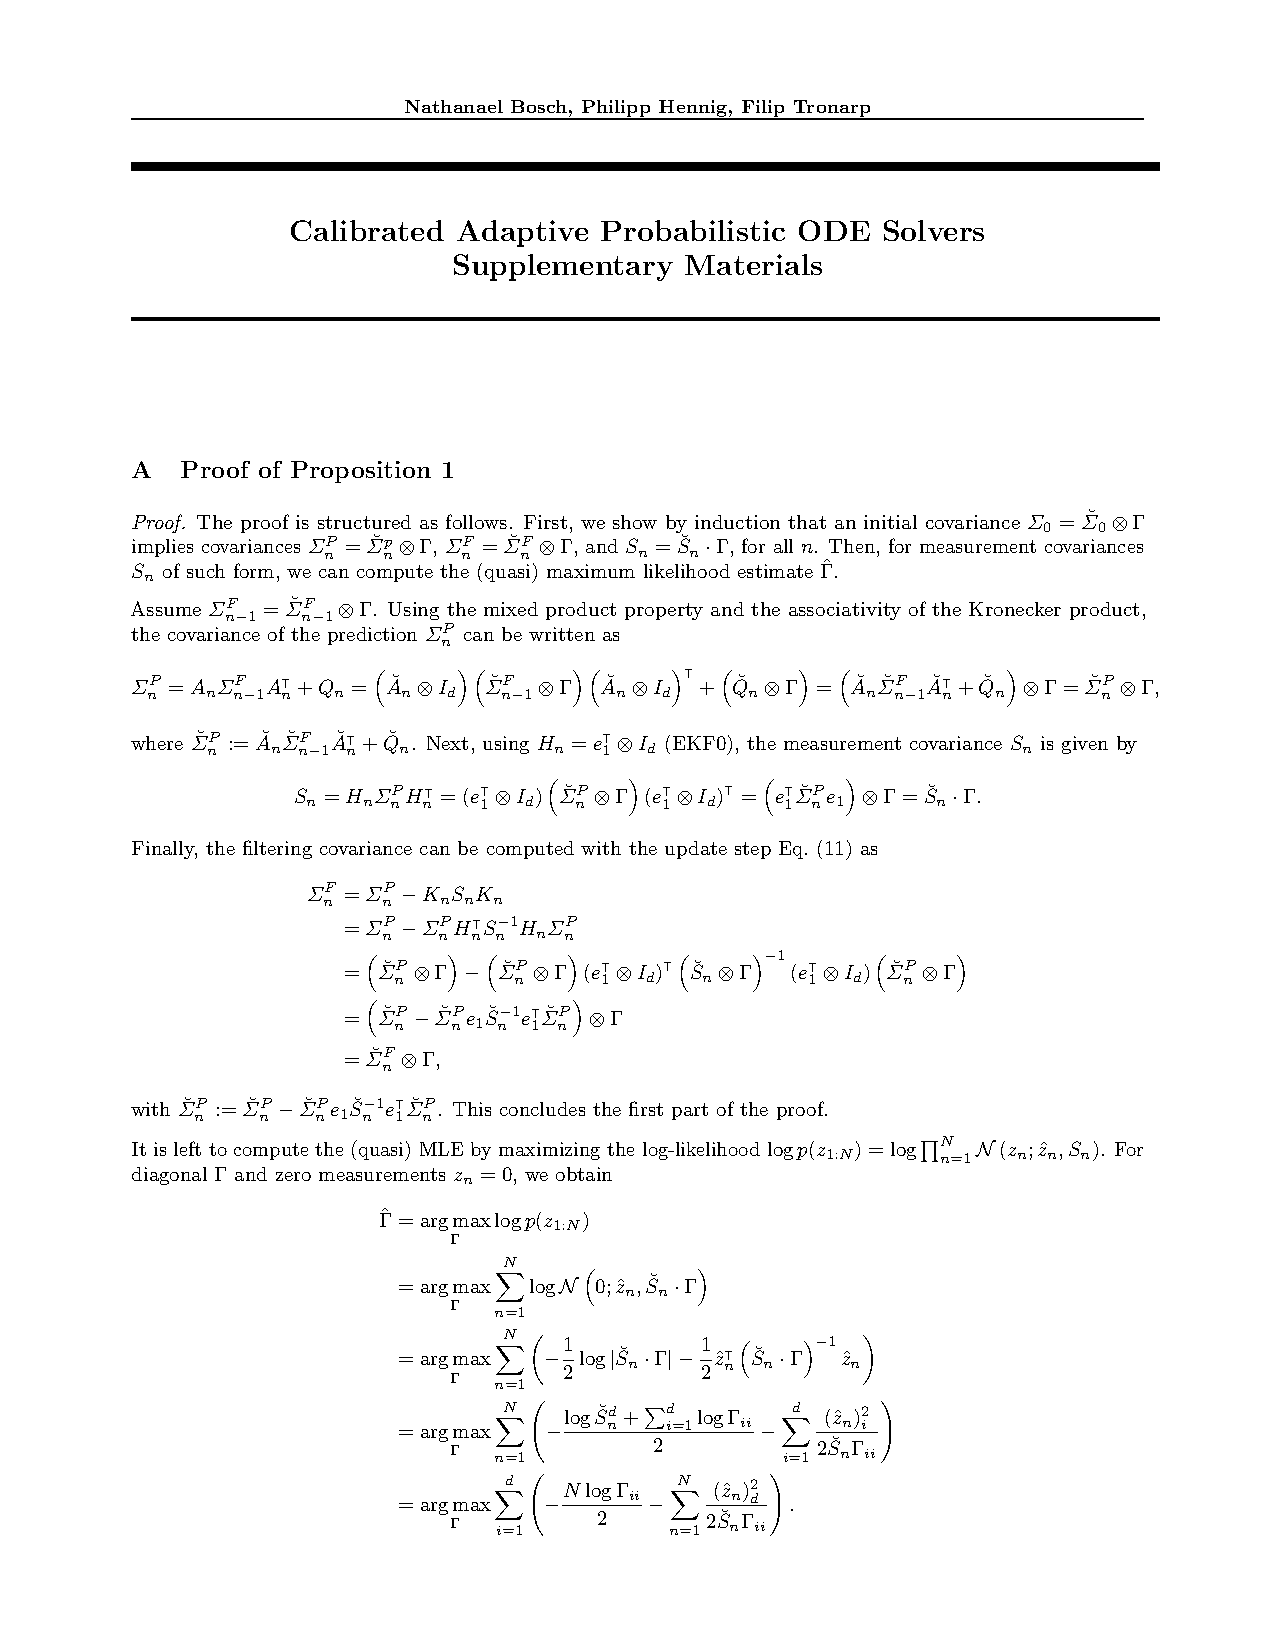
\includepdf[pages=-,pagecommand={}]{papers/capos-supp.pdf}

\includepaper{papers/pickandmix.pdf}{
Pick-and-mix information operators for probabilistic ODE solvers
\parencite{bosch21_pick_and_mix_infor_operat}
}{paper:pickandmix}

\includepaper{papers/highdim.pdf}{
Probabilistic ODE solutions in millions of dimensions
\parencite{krämer2021probabilistic}
}{paper:highdim}

\includepaper{papers/fenrir.pdf}{
Fenrir: Physics-enhanced regression for initial value problems
\parencite{tronarp2022fenrir}
}{paper:fenrir}

\includepaper{papers/probexpint.pdf}{
Probabilistic exponential integrators
\parencite{bosch2023probabilistic}
}{paper:probexpint}

\includepaper{papers/tempering.pdf}{
Diffusion Tempering Improves Parameter Estimation with Probabilistic Integrators for Ordinary Differential Equations
\parencite{beck2024diffusion}
}{paper:probexpint}

\includepaper{papers/parallel-in-time.pdf}{
Parallel-in-time probabilistic numerical ODE solvers
\parencite{bosch2023parallelintime}
}{paper:parallel-in-time}

\includepaper{papers/joss.pdf}{
ProbNumDiffEq.jl: Probabilistic numerical solvers for ordinary differential equations in Julia
\parencite{bosch2024joss}
}{paper:joss}
\end{document}
